% !TeX encoding = UTF-8
% !TeX program = xelatex
% !TeX spellcheck = en_US

\documentclass[degree=master]{thuthesis}
  % 学位 degree:
  %   doctor | master | bachelor | postdoc
  % 学位类型 degree-type:
  %   academic(默认)| professional
  % 语言 language
  %   chinese(默认)| english
  % 字体库 fontset
  %   windows | mac | fandol | ubuntu
  % 建议终版使用 Windows 平台的字体编译


% 论文基本配置,加载宏包等全局配置
% !TeX root = ./thuthesis-example.tex

% 论文基本信息配置

\thusetup{
  %******************************
  % 注意:
  %   1. 配置里面不要出现空行
  %   2. 不需要的配置信息可以删除
  %   3. 建议先阅读文档中所有关于选项的说明
  %******************************
  %
  % 输出格式
  %   选择打印版(print)或用于提交的电子版(electronic),前者会插入空白页以便直接双面打印
  %
  output = print,
  % 格式类型
  %   默认为论文(thesis),也可以设置为开题报告(proposal)
  % thesis-type = proposal,
  %
  % 标题
  %   可使用“\\”命令手动控制换行
  %
  title  = {量子线路的观测值模拟},
  title* = {Simulating observables of quantum circuits},
  %
  % 学科门类
  %   1. 学术型
  %      - 中文
  %        需注明所属的学科门类,例如:
  %        哲学、经济学、法学、教育学、文学、历史学、理学、工学、农学、医学、
  %        军事学、管理学、艺术学
  %      - 英文
  %        博士:Doctor of Philosophy
  %        硕士:
  %          哲学、文学、历史学、法学、教育学、艺术学门类,公共管理学科
  %          填写“Master of Arts“,其它填写“Master of Science”
  %   2. 专业型
  %      直接填写专业学位的名称,例如:
  %      教育博士、工程硕士等
  %      Doctor of Education, Master of Engineering
  %   3. 本科生不需要填写
  %
  degree-category  = {理学博士},
  degree-category* = {Doctor of Philosophy},
  %
  % 培养单位
  %   填写所属院系的全名
  %
  department = {数学科学系},
  %
  % 学科
  %   1. 研究生学术型学位,获得一级学科授权的学科填写一级学科名称,其他填写二级学科名称
  %   2. 本科生填写专业名称,第二学位论文需标注“(第二学位)”
  %
  discipline  = {数学},
  discipline* = {Mathmathics},
  %
  % 专业领域
  %   1. 设置专业领域的专业学位类别,填写相应专业领域名称
  %   2. 2019 级及之前工程硕士学位论文,在 `engineering-field` 填写相应工程领域名称
  %   3. 其他专业学位类别的学位论文无需此信息
  %
  % professional-field  = {计算机技术},
  % professional-field* = {Computer Technology},
  %
  % 姓名
  %
  author  = {邵钰菓},
  author* = {Yuguo Shao},
  %
  % 学号
  % 仅当书写开题报告时需要(同时设置 `thesis-type = proposal')
  %
  % student-id = {2000310000},
  %
  % 指导教师
  %   中文姓名和职称之间以英文逗号“,”分开,下同
  %
  supervisor  = {刘正伟, 教授},
  supervisor* = {Professor Zhengwei Liu},
  %
  % 副指导教师
  %
  %associate-supervisor  = {陈文光, 教授},
  %associate-supervisor* = {Professor Chen Wenguang},
  %
  % 联合指导教师
  %
  % co-supervisor  = {某某某, 教授},
  % co-supervisor* = {Professor Mou Moumou},
  %
  % 日期
  %   使用 ISO 格式;默认为当前时间
  %
  % date = {2019-07-07},
  %
  % 是否在中文封面后的空白页生成书脊(默认 false)
  %
  include-spine = false,
  %
  % 密级和年限
  %   秘密, 机密, 绝密
  %
  % secret-level = {秘密},
  % secret-year  = {10},
  %
  % 博士后专有部分
  %
  % clc                = {分类号},
  % udc                = {UDC},
  % id                 = {编号},
  % discipline-level-1 = {计算机科学与技术},  % 流动站(一级学科)名称
  % discipline-level-2 = {系统结构},          % 专业(二级学科)名称
  % start-date         = {2011-07-01},        % 研究工作起始时间
}

% 载入所需的宏包

% 定理类环境宏包
\usepackage{amsthm}
% 也可以使用 ntheorem
% \usepackage[amsmath,thmmarks,hyperref]{ntheorem}

\thusetup{
  %
  % 数学字体
  % math-style = GB,  % GB | ISO | TeX
  math-font  = xits,  % stix | xits | libertinus
}

% 可以使用 nomencl 生成符号和缩略语说明
% \usepackage{nomencl}
% \makenomenclature

% 表格加脚注
\usepackage{threeparttable}

% 表格中支持跨行
\usepackage{multirow}
\usepackage{physics}
% 固定宽度的表格。
% \usepackage{tabularx}

% 跨页表格
\usepackage{longtable}

% 算法
\usepackage{algorithm}
\usepackage{algorithmic}

% 量和单位
\usepackage{siunitx}
\usepackage{quantikz}

% 参考文献使用 BibTeX + natbib 宏包
% 顺序编码制
\usepackage[sort]{natbib}
\bibliographystyle{thuthesis-numeric}

% 著者-出版年制
% \usepackage{natbib}
% \bibliographystyle{thuthesis-author-year}

% 生命科学学院要求使用 Cell 参考文献格式(2023 年以前使用 author-date 格式)
% \usepackage{natbib}
% \bibliographystyle{cell}

% 本科生参考文献的著录格式
% \usepackage[sort]{natbib}
% \bibliographystyle{thuthesis-bachelor}

% 参考文献使用 BibLaTeX 宏包
% \usepackage[style=thuthesis-numeric]{biblatex}
% \usepackage[style=thuthesis-author-year]{biblatex}
% \usepackage[style=gb7714-2015]{biblatex}
% \usepackage[style=apa]{biblatex}
% \usepackage[style=mla-new]{biblatex}
% 声明 BibLaTeX 的数据库
% \addbibresource{ref/refs.bib}

% 定义所有的图片文件在 figures 子目录下
\graphicspath{{figures/}}

% 数学命令
\makeatletter
\newcommand\dif{%  % 微分符号
  \mathop{}\!%
  \ifthu@math@style@TeX
    d%
  \else
    \mathrm{d}%
  \fi
}
\makeatother

% hyperref 宏包在最后调用
\usepackage{hyperref}

\newcommand{\supp}{\text{supp}}
\newcommand{\poly}{\text{Poly}}


\begin{document}

% 封面
\maketitle

% 学位论文指导小组、公开评阅人和答辩委员会名单
% 本科生不需要
% !TeX root = ../thuthesis-example.tex

%\begin{committee}[name={学位论文指导小组、公开评阅人和答辩委员会名单}]
\begin{committee}[name={学位论文公开评阅人和答辩委员会名单}]
  \newcolumntype{C}[1]{@{}>{\centering\arraybackslash}p{#1}}

  \section*{指导小组名单}

  \begin{center}
    \begin{tabular}{C{3cm}C{3cm}C{9cm}@{}}
      刘正伟 & 教授     & 清华大学 
  %    王XX & 副教授   & 清华大学 \\
  %    张XX & 助理教授 & 清华大学 \\
    \end{tabular}
  \end{center}


  \section*{公开评阅人名单}

  \begin{center}
    \begin{tabular}{C{3cm}C{3cm}C{9cm}@{}}
      骆顺龙	& 研究员   & 中国科学院数学与系统科学研究院\\
      魏朝晖 & 助理教授 & 清华大学\\
      张潘 & 研究员 & 中国科学院理论物理研究所 \\
      袁骁 & 助理教授 & 北京大学 
    \end{tabular}
  \end{center}


  \section*{答辩委员会名单}

  \begin{center}
    \begin{tabular}{C{2.75cm}C{2.98cm}C{4.63cm}C{4.63cm}@{}}
      主席 & 郑浩                  & 教授                    & 清华大学       \\
      委员 & 肖杰                  & 教授                    & 北京师范大学       \\
         & \multirow{2}{*}{骆顺龙} & \multirow{2}{*}{研究员} & 中国科学院 \\
         &                       &                         & 数学与系统科学研究院  \\
        %& 骆顺龙                  & 研究员                    & 中国科学院数学与系统科学研究院       \\
          & 左怀青                  & 教授                  & 清华大学       \\
          & 魏朝晖                  & 助理教授                  & 清华大学       \\
      秘书 & 李慧慧                  & 博士后              & 清华大学       \\
    \end{tabular}
  \end{center}
\end{committee}



% 也可以导入 Word 版转的 PDF 文件
% \begin{committee}[file=figures/committee.pdf]
% \end{committee}


% 使用授权的说明
% 本科生开题报告不需要
\copyrightpage
% 将签字扫描后授权文件 scan-copyright.pdf 替换原始页面
% \copyrightpage[file=scan-copyright.pdf]

\frontmatter
% !TeX root = ../thuthesis-example.tex

% 中英文摘要和关键字

\begin{abstract}
  量子计算的经典模拟是验证量子硬件、优化算法设计及探索量子优势边界的重要工具。本文针对含噪声中等规模量子(NISQ)设备的模拟需求,提出基于Pauli路径积分的高效经典模拟方法,系统分析其计算复杂度与误差特性,并验证其实际应用价值。

  大规模变分量子算法被广泛认为是实现实用量子优势的潜在途径。然而,量子噪声的存在可能会抑制并削弱这些优势,这使得经典可模拟性的界限变得模糊。为了进一步澄清这一问题,我们提出了一种基于可观测量在泡利路径上反向传播路径积分(OBPPP)的新型多项式规模方法。该方法能够在单量子比特泡利噪声存在的情况下,以有界截断误差高效近似变分量子算法中算子的期望值。理论上我们严格证明:1)当最小非零噪声率γ为常数时,OBPPP的时间与空间复杂度与量子比特数n、电路深度L呈现多项式关系;2)对于可变的γ,当存在超过两个非零噪声因子时,若γ大于1/log L则复杂度保持Poly(n, L),但若γ低于1/L时复杂度将随L呈指数增长。数值方面,我们对IBM在127量子比特鹰处理器上进行的零噪声外推实验结果[Nature 618, 500 (2023)]进行了经典模拟。相比量子设备,我们的方法获得了更高的精度与更快的运行速度。此外,我们的方法能够模拟含噪声结果,精确复现了IBM未经误差缓解、与原始实验观测直接对应的计算结果。本研究表明噪声在经典模拟中的关键作用,所提出的方法适用于广泛量子电路的期望值计算,在量子计算机验证领域具有普适性。



  论文的摘要是对论文研究内容和成果的高度概括。
  摘要应对论文所研究的问题及其研究目的进行描述,对研究方法和过程进行简单介绍,对研究成果和所得结论进行概括。
  摘要应具有独立性和自明性,其内容应包含与论文全文同等量的主要信息。
  使读者即使不阅读全文,通过摘要就能了解论文的总体内容和主要成果。

  论文摘要的书写应力求精确、简明。
  切忌写成对论文书写内容进行提要的形式,尤其要避免“第 1 章……;第 2 章……;……”这种或类似的陈述方式。

  关键词是为了文献标引工作、用以表示全文主要内容信息的单词或术语。
  关键词不超过 5 个,每个关键词中间用分号分隔。

  % 关键词用“英文逗号”分隔,输出时会自动处理为正确的分隔符
  \thusetup{
    keywords = {量子计算, 量子线路经典模拟 , Pauli路径积分, 变分量子算法, 量子噪声},
  }
\end{abstract}

\begin{abstract*}
  An abstract of a dissertation is a summary and extraction of research work and contributions.
  Included in an abstract should be description of research topic and research objective, brief introduction to methodology and research process, and summary of conclusion and contributions of the research.
  An abstract should be characterized by independence and clarity and carry identical information with the dissertation.
  It should be such that the general idea and major contributions of the dissertation are conveyed without reading the dissertation.

  An abstract should be concise and to the point.
  It is a misunderstanding to make an abstract an outline of the dissertation and words “the first chapter”, “the second chapter” and the like should be avoided in the abstract.

  Keywords are terms used in a dissertation for indexing, reflecting core information of the dissertation.
  An abstract may contain a maximum of 5 keywords, with semi-colons used in between to separate one another.

  % Use comma as separator when inputting
  \thusetup{
    keywords* = {keyword 1, keyword 2, keyword 3, keyword 4, keyword 5},
  }
\end{abstract*}


% 目录
\tableofcontents

% 插图和附表清单
% 本科生的插图索引和表格索引需要移至正文之后、参考文献前
% \listoffiguresandtables  % 插图和附表清单(仅限研究生)
\listoffigures           % 插图清单
\listoftables            % 附表清单

% 符号对照表
% !TeX root = ../thuthesis-example.tex

\begin{denotation}[3cm]
  \item[CPD] Clifford数据回归(Clifford Data Regression)
  \item[CPDR] Clifford扰动数据回归(Clifford Perturbation Data Regression)
  \item[CPTP] 完全正保迹(Completely Positive and Trace-Preserving) 
  \item[DMRG] 密度矩阵重整化群(Density Matrix Renormalization Group)
  \item[MPS] 矩阵乘积态(Matrix Product State) 
  \item[MSE] 均方误差(Mean Squared Error) 
  \item[NISQ] 含噪声中等规模量子(Noisy Intermediate-Scale Quantum)
  \item[OBPPP] 可观测量在Pauli路径下的反向传播算法(Observable's Back-Propagation on Pauli Path)
  \item[POVM] 正算子值测量(Positive Operator-Valued Measure)
  \item[QAOA] 量子近似优化算法(Quantum Approximate Optimization Algorithm)
  \item[QEC] 量子纠错(Quantum Error Correction)
  \item[Qubit] 量子比特(Quantum Bit)
  \item[QSVM] 量子支持向量机(Quantum Support Vector Machine) 
  \item[QNN] 量子神经网络(Quantum Neural Network) 
  \item[RRMSE] 相对均方根误差(Relative Root Mean Square Error) 
  \item[SPD] 稀疏Pauli动力学 (Sparse Pauli Dynamics)
  \item[SVD] 奇异值分解(Singular Value Decomposition)
  \item[VQA] 变分量子算法(Variational Quantum Algorithm) 
  \item[VQE] 变分量子本征求解器(Variational Quantum Eigensolver)
  \item[ZNE] 零噪声推断(Zero-Noise Extrapolation)
  
  
\end{denotation}



% 也可以使用 nomencl 宏包,需要在导言区
% \usepackage{nomencl}
% \makenomenclature

% 在这里输出符号说明
% \printnomenclature[3cm]

% 在正文中的任意为都可以标题
% \nomenclature{PI}{聚酰亚胺}
% \nomenclature{MPI}{聚酰亚胺模型化合物,N-苯基邻苯酰亚胺}
% \nomenclature{PBI}{聚苯并咪唑}
% \nomenclature{MPBI}{聚苯并咪唑模型化合物,N-苯基苯并咪唑}
% \nomenclature{PY}{聚吡咙}
% \nomenclature{PMDA-BDA}{均苯四酸二酐与联苯四胺合成的聚吡咙薄膜}
% \nomenclature{MPY}{聚吡咙模型化合物}
% \nomenclature{As-PPT}{聚苯基不对称三嗪}
% \nomenclature{MAsPPT}{聚苯基不对称三嗪单模型化合物,3,5,6-三苯基-1,2,4-三嗪}
% \nomenclature{DMAsPPT}{聚苯基不对称三嗪双模型化合物(水解实验模型化合物)}
% \nomenclature{S-PPT}{聚苯基对称三嗪}
% \nomenclature{MSPPT}{聚苯基对称三嗪模型化合物,2,4,6-三苯基-1,3,5-三嗪}
% \nomenclature{PPQ}{聚苯基喹噁啉}
% \nomenclature{MPPQ}{聚苯基喹噁啉模型化合物,3,4-二苯基苯并二嗪}
% \nomenclature{HMPI}{聚酰亚胺模型化合物的质子化产物}
% \nomenclature{HMPY}{聚吡咙模型化合物的质子化产物}
% \nomenclature{HMPBI}{聚苯并咪唑模型化合物的质子化产物}
% \nomenclature{HMAsPPT}{聚苯基不对称三嗪模型化合物的质子化产物}
% \nomenclature{HMSPPT}{聚苯基对称三嗪模型化合物的质子化产物}
% \nomenclature{HMPPQ}{聚苯基喹噁啉模型化合物的质子化产物}
% \nomenclature{PDT}{热分解温度}
% \nomenclature{HPLC}{高效液相色谱(High Performance Liquid Chromatography)}
% \nomenclature{HPCE}{高效毛细管电泳色谱(High Performance Capillary lectrophoresis)}
% \nomenclature{LC-MS}{液相色谱-质谱联用(Liquid chromatography-Mass Spectrum)}
% \nomenclature{TIC}{总离子浓度(Total Ion Content)}
% \nomenclature{\textit{ab initio}}{基于第一原理的量子化学计算方法,常称从头算法}
% \nomenclature{DFT}{密度泛函理论(Density Functional Theory)}
% \nomenclature{$E_a$}{化学反应的活化能(Activation Energy)}
% \nomenclature{ZPE}{零点振动能(Zero Vibration Energy)}
% \nomenclature{PES}{势能面(Potential Energy Surface)}
% \nomenclature{TS}{过渡态(Transition State)}
% \nomenclature{TST}{过渡态理论(Transition State Theory)}
% \nomenclature{$\increment G^\neq$}{活化自由能(Activation Free Energy)}
% \nomenclature{$\kappa$}{传输系数(Transmission Coefficient)}
% \nomenclature{IRC}{内禀反应坐标(Intrinsic Reaction Coordinates)}
% \nomenclature{$\nu_i$}{虚频(Imaginary Frequency)}
% \nomenclature{ONIOM}{分层算法(Our own N-layered Integrated molecular Orbital and molecular Mechanics)}
% \nomenclature{SCF}{自洽场(Self-Consistent Field)}
% \nomenclature{SCRF}{自洽反应场(Self-Consistent Reaction Field)}



% 正文部分
\mainmatter
\chapter{绪论}

\section{研究背景}

量子力学的建立和发展是20世纪人类科学领域最伟大的科学突破之一,它不仅解决了经典物理学在描述微观世界中的失败,而且在许多方面都超越了经典物理学。量子力学的建立不仅推动了物理学的发展,而且对其他学科的发展也产生了深远的影响,许多新兴的领域和学科就此产生,如量子信息科学。

量子信息科学是量子力学和信息科学的交叉领域,它主要研究如何利用量子力学的特性来处理和传输信息。在当今信息时代,信息的处理和传输已经成为人们生活中不可或缺的一部分。
自1940年代,第一台电子计算机诞生以来,计算机技术已经取得了长足的进步,计算机的性能也在不断提高。
英特尔公司创始人戈登·摩尔在1965年提出的摩尔定律,预言单个集成电路上可容纳的晶体管数目每隔18个到24个月就会翻一番。
这一定律不是一个自然定律,而是人们在经验上总结出来的一个规律,但是在过去的几十年中,摩尔定律一直被证明是正确的。但是随着计算机技术的不断发展,集成电路的尺寸越来越小,逐渐接近原子尺度。
在原子尺度下,经典物理学的规律不再适用,量子效应开始显现,这就导致了集成电路的性能难以继续提高,摩尔定律也逐渐失效。

而随着人工智能、大数据、物联网等新兴技术的发展,对计算机性能的需求也越来越高。在这种情况下,传统的计算机技术已经无法满足人们的需求,因此人们开始寻找新的计算机技术。量子计算机作为一种新型的计算机技术,具有很大的发展潜力,并被认为是未来计算机技术的发展方向之一。

在1980年代,Benioff、Manin、Feynman等人提出了量子计算机的概念~\cite{Benioff1980,Benioff1982a,Benioff1982b,Manin1980,Feynman1982}。
最初的动机是希望利用量子力学的特性来模拟量子系统,如果使用经典计算机来模拟量子系统,需要耗费大量的计算资源,而量子计算机可以更加高效地模拟量子系统。后来的研究表明,量子计算机不仅可以模拟量子系统,而且可以解决一些经典计算机难以处理的问题。
1994年,Shor提出了一种基于量子计算机的大整数分解算法~\cite{shor1994algorithms},该算法可以在多项式时间内分解大整数,这对于现代密码学体系具有重要意义。
时至今日,量子计算的研究吸引了众多科学家的关注,也在各个领域衍生出了广泛的应用,包括密码学、量子化学~\cite{peruzzo2014variational, Kandala2017hardware,li2022toward}、量子机器学习~\cite{beer2020training,huang2021experimental,havlivcek2019supervised,mitarai2018quantum}、量子优化算法~\cite{farhi2014quantum,moll2018quantum}等。
此外,除了量子计算之外,量子信息还包括量子纠错、量子复杂度、量子通信、量子传感、量子控制等领域,这些领域也为量子信息科学的发展提供了新的思路和方法。

随着实验技术的进步,量子计算机的实际实现也取得了长足的进步。现在基于各种不同的物理系统,包括离子阱、超导量子比特、量子点、拓扑量子比特等,各种量子计算机的实验平台已经相继建立~\cite{blatt2008quantum,devoret2013superconducting,wallraff2004strong,loss1998quantum}。自2019年以来,研究人员相继在超导量子比特、光量子等平台展示了量子计算在特定任务上对经典计算机的超越,实现了包括随机线路采样~\cite{arute2019quantum}、高斯波色采样等~\cite{zhong2020quantum}等特定任务的量子优越性验证。
近些年来,量子计算机已经发展到了含噪声中等规模量子(Noisy Intermediate-Scale Quantum, NISQ)阶段,这一阶段的量子计算机拥有数十到数百个量子比特,暂无法实现完全容错的量子计算,但是拥有在特定任务上超越经典计算机的潜力。

另一方面,量子计算机的发展也面临着许多困难和挑战。量子计算机的硬件系统非常脆弱,容易受到外界干扰,导致量子比特发生错误。保护量子比特免受外界干扰是量子计算机研究的一个重要课题,量子纠错技术(Quantum Error Correction,QEC)就是为了解决这个问题,通过将量子信息编码在纠错码中,可以有效地保护量子比特免受外界干扰。量子纠错技术是量子计算机研究的一个重要方向,也是实现大规模量子计算的关键技术之一。
噪声阈值定理保证了只要量子比特的错误率低于某个阈值,就可以通过扩大纠错码的规模来实现任意精度的量子计算~\cite{aharonov1997fault,aliferis2008fault}。
近期,研究人员先后在光量子、超导量子平台上取得了里程碑式的量子纠错实验进展,展示了低于噪声阈值的量子纠错~\cite{ni2023beating,acharya2024quantum,sivak2023real}。
尽管量子计算已经取得了长足的进步,但是要实现大规模量子计算仍然面临着许多困难和挑战,若要真正在生产环境中应用量子计算,还需要解决许多问题,还需要持续在理论和实验方面继续探索和研究。


\section{量子力学简介}
量子力学的建立源于19世纪末20世纪初,当时的物理学家们在研究原子和分子的结构时,发现了一些经典物理学无法解释的现象,如黑体辐射、光电效应、电子的双缝干涉等。20世纪初,普朗克、爱因斯坦、德布罗意、玻尔等人相继提出了量子假设、光量子假设、波粒二象性等概念,奠定了量子力学的基础。
在本节中,我们将简要介绍与量子计算相关的量子力学基础知识,包括量子比特、量子态、量子门、量子纠错等。

\subsection{量子态与密度矩阵}

对于一个纯态量子系统,它在某一时刻的状态可以用一个希尔伯特空间中的一个矢量来表示,称为量子态矢量,利用Dirac符号表示为$|\psi\rangle$。Dirac符号$|\psi\rangle$的数学形式等价于一个N维复线形空间中的列向量,其中N是希尔伯特空间的维度,$|\psi\rangle$称为右矢,代表列向量;$\langle\psi|$称为左矢,代表行向量。两者之间互为共轭转置关系,即$\langle\psi| = |\psi\rangle^\dagger$,其中$\dagger$表示共轭转置。两个量子态之间的内积和外积分别表示为$\langle\psi|\phi\rangle$和$|\psi\rangle\langle\phi|$。

对于一个$N$维空间的量子系统,它的状态可以表示为一个$N$维复数向量,即$\mathbb{C}^N$中的一个矢量:
\begin{equation}
    |\psi\rangle = \begin{pmatrix} \alpha_0 \\ \alpha_1 \\ \cdots \\ \alpha_{N-1} \end{pmatrix} = \sum_{i=0}^{N-1} \alpha_i|\phi_i\rangle,
\end{equation}
其中$\alpha_i$是复数,满足$\sum_{i=0}^{N-1} |\alpha_i|^2 = 1$,$\{|\phi_i\rangle\}$是希尔伯特空间的一组完备的正交归一基矢。
完备性条件$\sum_{i=0}^{N-1} |\phi_i\rangle\langle\phi_i| = I$,其中$I$是单位算符。正交性条件$\langle\phi_i|\phi_j\rangle = \delta_{ij}$,其中$\delta_{ij}$是Kronecker delta符号。


对于多个系统构成的复合系统,它的状态可以表示为各个子系统状态的张量积,即
\begin{equation}
    |\psi\rangle = |\psi_1\rangle \otimes |\psi_2\rangle \otimes \cdots \otimes |\psi_n\rangle,
\end{equation}
其中$|\psi_i\rangle$是第$i$个子系统的状态。
因此组合系统中量子态的维度是各个子系统维度的乘积,即$N = N_1 \times N_2 \times \cdots \times N_n$。

对于一个量子系统,它的状态可以是纯态或混合态。纯态是指量子系统处于一个确定的态,可以用上述的矢量来描述;混合态是指量子系统处于一个不确定的态,需要用密度矩阵来描述。密度矩阵是一个厄米矩阵,它可以描述量子系统的统计性质,对于一个纯态量子系统,它的密度矩阵定义为
\begin{equation}
    \rho = |\psi\rangle\langle\psi|,
\end{equation}
其中$|\psi\rangle$是量子系统的状态矢量。对于一个混合态,假设量子系统处于一组纯态$|\psi_i\rangle$的概率为$p_i$,则它的密度矩阵定义为
\begin{equation}
    \rho = \sum_i p_i |\psi_i\rangle\langle\psi_i|,
\end{equation}
其中$p_i$是量子系统处于第$i$个纯态的概率,满足$\sum_i p_i = 1$。


在量子力学中,对N维空间的量子系统,密度矩阵满足以下性质:
\begin{enumerate}
    \item 密度矩阵$\rho\in \mathcal{L}(\mathbb{C}^N)$是一个厄米矩阵,即$\rho = \rho^\dagger$;
    \item 密度矩阵是正定的,即对于任意的态矢量$|\psi\rangle$,有$\langle\psi|\rho|\psi\rangle \geq 0$;
    \item 密度矩阵的迹为1,即$\Tr(\rho) = 1$。
\end{enumerate}

对于所有态的均匀混合态,即$\rho = \int d\mu(\lambda) |\lambda\rangle\langle\lambda|$,其中$d\mu(\lambda)$是一个概率测度,满足$\int d\mu(\lambda) = 1$。当概率测度$d\mu(\lambda)$取常用的Haar测度时,这样的密度矩阵称为最大混合态。最大混合态是一个对角矩阵,对角元素都是相等的,即$\rho = \frac{1}{N}I$,其中$N$是希尔伯特空间的维度,$I$是单位算符。
最大混合态常用于描述量子系统的混沌性质,它是量子系统的最大不确定态,对于任意的测量,最大混合态的测量结果是完全随机的。

\subsection{量子态演化}
量子态的演化是量子计算中的一个重要问题,它描述了量子系统在不同时间点的状态之间的关系。在量子力学中,一个封闭系统的演化是由系统的哈密顿量(Hamiltonian)决定的,t时刻的哈密顿量记为$H(t)$,它描述了系统的动力学性质,满足厄米性质$H(t) = H(t)^\dagger$。孤立系统的随时间的演化可以用薛定谔方程(Schrödinger Equation)来描述,即
\begin{equation}
    i\hbar\frac{\partial}{\partial t}|\psi(t)\rangle = H(t)|\psi(t)\rangle,
\end{equation}
其中$\hbar$是约化普朗克常数,$|\psi(t)\rangle$是系统在时间$t$的状态。薛定谔方程的解可以表示为
\begin{equation}
    |\psi(t)\rangle = U(t)|\psi(0)\rangle,
\end{equation}
其中$U(t) = \exp\left(-\frac{i}{\hbar}\int_0^t H(t')dt'\right)$是时间演化算符,它描述了系统从初始状态$|\psi(0)\rangle$到时间$t$的状态$|\psi(t)\rangle$之间的关系。
时间演化算符$U(t)$是一个幺正算符,满足$U(t)U^\dagger(t) = U^\dagger(t)U(t) = I$。


如果采用密度矩阵来描述量子系统,那么密度矩阵的演化可以用薛定谔方程的密度矩阵形式来描述,即
\begin{equation}
    i\hbar\frac{\partial}{\partial t}\rho(t) = [H(t), \rho(t)],
\end{equation}
其中$[\cdot, \cdot]$表示两个算符的对易子。密度矩阵的演化可以表示为
\begin{equation}
    \rho(t) = U(t)\rho(0)U^\dagger(t).
\end{equation}

\subsection{量子测量}
量子测量是量子力学中的一个重要概念,它描述了量子系统在测量过程中的状态演化。在量子力学中,测量是一个不可逆的过程,它会导致量子系统的状态坍缩。在量子力学中,一个量子系统的可观测量是一个厄米算符$O$,满足$O=\sum_i \lambda_i M_i$,其中$\{M_i\}$是一组半正定厄米算符,满足$M_i \geq 0,M_i=M_i^\dagger$和完备性$\sum_i M_i = I$。因为$M_i \geq 0$,所以存在$\{E_i\}$使得$M_i = E_i^\dagger E_i$,这样的测量算符称为正算子(Positive Operator)。
在量子系统的正算子值测量(Positive Operator-Valued Measure, POVM)过程中,量子系统的状态会坍缩到测量结果对应的态上,即
\begin{equation}
    \rho \rightarrow \frac{E_i\rho E_i^\dagger}{\Tr(E_i\rho E_i^\dagger)},
\end{equation}
得到该状态的概率为$p_i = \Tr(E_i\rho E_i^\dagger)$。在测量过程中,测量结果是随机的,但是测量结果的概率是可以计算的。



通常我们关心的是可观测量的测量期望值,它可以表示为$\langle O \rangle$。期望值可以通过对量子态的多次重复测量得到,制备大量相同的量子态,对每个量子态进行测量,然后对测量结果求平均值。对纯态$\ket{\psi}$的可观测量$O$的期望值可以表示为
\begin{equation}
    \langle O \rangle = \langle \psi|O|\psi\rangle=\sum_i \lambda_i p_i=\sum_i \lambda_i \bra{\psi} E_i^\dagger E_i \ket{\psi},
\end{equation}
其中$p_i = \bra{\psi} E_i^\dagger E_i \ket{\psi}$是测量结果为$\lambda_i$的概率。对于混合态$\rho$,可观测量$O$的期望值可以表示为
\begin{equation}
    \langle O \rangle = \Tr(O\rho)=\sum_i \lambda_i \Tr(E_i\rho E_i^\dagger)=\sum_i \lambda_i \Tr(E_i\rho E_i^\dagger).
\end{equation}


\subsection{量子信道}
量子信道是量子信息科学中的一个重要概念,它描述了量子态在开放系统中的演化过程。
对于一个量子系统$A$,如果它与另一个量子系统$B$之间存在相互作用,那么系统$A$的状态会发生演化,这个相互作用可以用一个量子信道来描述。

假设联合系统$AB$的初始状态是$\rho_{AB} = \rho_A \otimes |\psi_0\rangle \langle \psi_0|$,系统$A$的初始状态是$\rho_A = \Tr_B(\rho_{AB})$,系统$B$的初始状态是$\rho_B = \Tr_A(\rho_{AB})=|\psi_0\rangle \langle \psi_0|$。
其中$\Tr_B$表示对系统$B$求偏迹,即对系统$B$的态矢量进行求和,得到系统$A$的密度矩阵;类似的$\Tr_A$表示对系统$A$求偏迹:
\begin{equation}
    \rho_A = \Tr_B(\rho_{AB}) = \sum_i \prescript{}{B}{\langle} \psi_i|\rho_{AB}|\psi_i\rangle_B, \quad \rho_B = \Tr_A(\rho_{AB}) = \sum_j \prescript{}{A}{\langle} \phi_j|\rho_{AB}|\phi_j\rangle_A,
\end{equation}
其中$\{|\psi_i\rangle_B\}$和$\{|\phi_j\rangle_A\}$分别是系统$B$和系统$A$的正交归一基矢。

假设系统$A$和系统$B$之间的相互作用可以用一个幺正算符$U$来描述,系统$A$的状态在相互作用后的状态可以表示为
\begin{equation}
    \rho_A' = \Tr_B(U\rho_{AB}U^\dagger) = \sum_i \prescript{}{B}{\langle} \psi_i|U\rho_{AB}U^\dagger|\psi_i\rangle_B.
\end{equation}

定义 Kraus 算符 $K_i = \prescript{}{B}{\langle} \psi_i|U|\psi_0\rangle_B$,则系统 $A$ 的最终状态可以表示为:
\begin{equation}
    \rho_A' = \sum_i K_i \rho_A K_i^\dagger.
\end{equation}
以上定义的 $K_i$ 满足 $\sum_i K_i^\dagger K_i = \sum_i \prescript{}{B}{\langle} \psi_i|U^\dagger U|\psi_0\rangle_B = I$.

对于一般的量子信道$\mathcal{T}$,可以用一组 Kraus 算符来描述,即
\begin{equation}
    \mathcal{T}(\rho) = \sum_i K_i \rho K_i^\dagger,
\end{equation}
其中 $\sum_i K_i^\dagger K_i = I$。量子信道的作用是将输入态 $\rho$ 映射到输出态 $\mathcal{T}(\rho)$。

Kraus算符保证了量子信道是完全正的,即保证了$\mathcal{T}\otimes I$是正映射,其中$I$是一个恒等算符。假设$\mathcal{T}$有Kraus表示$\mathcal{T}(\rho) = \sum_i K_i \rho K_i^\dagger$,则$\mathcal{T}\otimes I$作用在量子态$\rho=\sum_j \lambda_j \ketbra{\phi_j}$上,有:
\begin{equation}
        \mathcal{T}\otimes I(\rho) = \sum_i (K_i \otimes I)(\rho)(K_i \otimes I)^\dagger = \sum_i (K_i \otimes I)(\sum_j \lambda_j \ketbra{\phi_j})(K_i \otimes I)^\dagger.
\end{equation}
则对于任意的态$\ket{\psi}$,有
\begin{equation}
    \begin{aligned}
        \bra{\psi}(\mathcal{T}\otimes I)(\rho)\ket{\psi} &= \sum_{i,j} \lambda_j \bra{\psi}(K_i \otimes I)\ket{\phi_j}\bra{\phi_j}(K_i \otimes I)^\dagger\ket{\psi} \\
        &= \sum_{i,j} \lambda_j \bra{\psi}(K_i \otimes I)\ket{\phi_j}\bra{\phi_j}(K_i^\dagger \otimes I)\ket{\psi} \\
        &= \sum_{i,j} \lambda_j |\bra{\psi}(K_i \otimes I)\ket{\phi_j}|^2 \geq 0.
    \end{aligned}
\end{equation}
因此,$\mathcal{T}\otimes I$是正的,即$\mathcal{T}$是完全正的。

此外$\sum_i K_i^\dagger K_i = I$保证了量子信道是保迹的,即保证了$\Tr(\mathcal{T}(\rho)) = \Tr(\rho)$。这是因为
\begin{equation}
    \begin{aligned}
        \Tr(\mathcal{T}(\rho)) &= \Tr(\sum_i K_i \rho K_i^\dagger) = \sum_i \Tr(K_i \rho K_i^\dagger) = \sum_i \Tr(\rho K_i^\dagger K_i) \\
        &= \Tr(\rho I) = \Tr(\rho).
    \end{aligned}
\end{equation}

这样完全正的保迹(Completely Positive and Trace-Preserving, CPTP)映射刻画了一般的量子信道的性质,它描述了量子态在开放系统中的演化过程。


\section{量子计算简介}

量子计算是一种基于量子力学原理的计算模型,它利用量子力学的特性来处理和传输信息。
类比经典计算的基本要素如比特、逻辑门、线路等,量子计算也有类似的基本要素。

\subsection{量子比特}
量子比特(Quantum Bit, Qubit)是量子计算的基本单元,它是量子力学中的最小信息单元,类似于经典计算中的比特(Bit)。
经典比特只能处于0或1两种状态,而量子比特可以处于0和1的叠加态,这通常是对应于二能级量子系统、或是多能级量子系统的两个特定的能级。
为了方便将两个能级记为$|0\rangle$和$|1\rangle$。在矩阵表示中,$|0\rangle$和$|1\rangle$分别表示为
\begin{equation}
    |0\rangle = \begin{pmatrix} 1 \\ 0 \end{pmatrix}, \quad |1\rangle = \begin{pmatrix} 0 \\ 1 \end{pmatrix}.
\end{equation}

一个任意量子比特的纯态可以表示为
\begin{equation}
    |\psi\rangle = e^{i\gamma}(\cos\frac{\theta}{2}|0\rangle + e^{i\phi}\sin\frac{\theta}{2}|1\rangle)=e^{i\gamma}\begin{pmatrix}
        \cos\frac{\theta}{2} \\ e^{i\phi}\sin\frac{\theta}{2}
    \end{pmatrix},
\end{equation}
其中$\theta$和$\phi$是两个角度,$\gamma$是一个全局相位,满足$0 \leq \theta \leq \pi$,$0 \leq \phi < 2\pi$,$0 \leq \gamma < 2\pi$。 单个量子比特的状态可以用Bloch球来表示,Bloch球是一个单位球,它的表面上的点对应于量子比特的纯态,如图~\ref{fig:bloch_sphere}所示。



\begin{figure}[H]
  \centering
  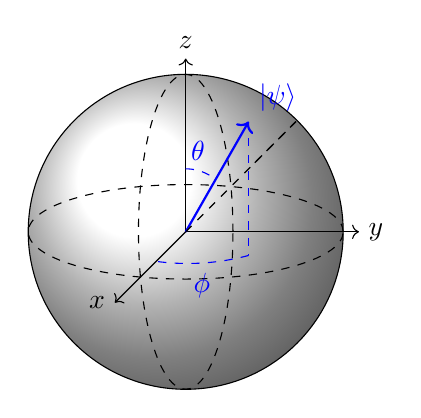
\begin{tikzpicture}
      % Draw the Bloch sphere
      \shade[ball color=white] (0,0) circle (2cm);
      \draw (0,0) circle (2cm);
      \draw[dashed] (0,0) circle (2cm and 0.6cm);
      \draw[dashed] (0,0) circle (0.6cm and 2cm);
      
      % Draw axes
      \draw[->] (0,0) -- (2.2,0) node[right] {$y$};
      \draw[->] (0,0) -- (0,2.2) node[above] {$z$};
      \draw[->] (0,0) -- (-0.9,-0.9) node[left] {$x$};
      
      % Draw state vector
      \draw[->,thick,blue] (0,0) -- (0.8,1.4) node[above right] {$|\psi\rangle$};
      
      % Draw angles
      \draw[dashed] (0,0) -- (1.4,1.4,0);
      \draw[dashed] (1.4,1.4,0) -- (1.4,1.4,1.4);
      \draw[dashed,blue] (0,0.8) arc (90:60:0.6) node[midway, above] {$\theta$};
      \draw[dashed,blue] (0.8,1.4) -- (0.8,-0.3);
      \draw[dashed,blue] (0.8,-0.3) arc (-75:-98:3) node[midway, below] {$\phi$};
  \end{tikzpicture}
  \caption{Bloch球表示}
  \label{fig:bloch_sphere}
\end{figure}

对于单个量子比特的混合态,它的密度矩阵可以表示为
\begin{equation}\label{eq:bloch_rho}
    \rho = \frac{1}{2}(I + \vec{r}\cdot\vec{\sigma}),
\end{equation}
其中$\vec{r} = (r_x, r_y, r_z)$是一个三维实向量,满足$|\vec{r}| \leq 1$,$\vec{\sigma} = (\sigma_x, \sigma_y, \sigma_z)$是Pauli矩阵,即
\begin{equation}
    \sigma_x = \begin{pmatrix} 0 & 1 \\ 1 & 0 \end{pmatrix}, \quad \sigma_y = \begin{pmatrix} 0 & -i \\ i & 0 \end{pmatrix}, \quad \sigma_z = \begin{pmatrix} 1 & 0 \\ 0 & -1 \end{pmatrix}.
\end{equation}
混合态对应的Bloch球上的点是一个三维实向量$\vec{r}$,它的长度小于等于1,即$|\vec{r}| \leq 1$。当$\norm{\vec{r}} = 1$时,即在Bloch球的表面上,对应的是一个纯态;当$\norm{\vec{r}} < 1$时,对应的点在Bloch球的内部,对应的是一个混合态。


一个由n个量子比特组成的量子系统有$2^n$个本征态,它的状态可以用长度为n的二进制串来表示,即$|x_1x_2\cdots x_n\rangle$,其中$x_i \in \{0, 1\}$。一个n量子比特的量子系统的状态可以表示为
\begin{equation}
    |\psi\rangle = \sum_{x=0}^{2^n-1} \alpha_x |x_1x_2\cdots x_n\rangle,
\end{equation}
其中$\alpha_x$是复数,满足$\sum_{x=0}^{2^n-1} |\alpha_x|^2 = 1$。
有时也会使用十进制表示,即$|x\rangle$,其中$x \in \{0, 1, \cdots, 2^n-1\}$。这样的基矢称为计算基矢(Computational Basis)。

\subsection{量子线路}
量子线路是量子计算中的一个重要概念,它描述了量子比特之间的相互作用关系。量子线路由量子门(Quantum Gate)组成,量子门是用来操作量子比特的基本单元,类似于经典计算中的逻辑门。量子门是一个幺正算符,它作用在量子比特上,改变量子比特的状态。

最简单的一类门是单比特量子门,常见的单比特量子门有Pauli门、Hadamard门、相位门、T门等。Pauli门是一组三个单比特门,分别是$X$门、$Y$门和$Z$门,它们的矩阵表示分别为
\begin{equation}
    X = \begin{pmatrix} 0 & 1 \\ 1 & 0 \end{pmatrix}, \quad Y = \begin{pmatrix} 0 & -i \\ i & 0 \end{pmatrix}, \quad Z = \begin{pmatrix} 1 & 0 \\ 0 & -1 \end{pmatrix}.
\end{equation}
Hadamard门是一个单比特门,常用于产生均匀叠加态,它常简记为H门,其矩阵表示为
\begin{equation}
    H = \frac{1}{\sqrt{2}}\begin{pmatrix} 1 & 1 \\ 1 & -1 \end{pmatrix}.
\end{equation}
上述的门矩阵表示既是幺正也是厄米的,因此既可以作为量子门,也可以作为测量算符。
另外还有两个常用的单比特门,分别是相位门(简记为$S$),还有T门,其矩阵表示分别为
\begin{equation}
    S = \begin{pmatrix} 1 & 0 \\ 0 & i \end{pmatrix}, \quad T = \begin{pmatrix} 1 & 0 \\ 0 & e^{i\pi/4} \end{pmatrix}.
\end{equation}

此外还有一类常用的含参数的单比特门,称为单比特旋转门,它们的矩阵表示为
\begin{equation}
    \begin{aligned}
        &R_X(\theta) =e^{-i\frac{\theta}{2}X} = \begin{pmatrix} \cos\frac{\theta}{2} & -i\sin\frac{\theta}{2} \\ -i\sin\frac{\theta}{2} & \cos\frac{\theta}{2} \end{pmatrix}, \\ &R_Y(\theta)=e^{-i\frac{\theta}{2}Y} = \begin{pmatrix} \cos\frac{\theta}{2} & -\sin\frac{\theta}{2} \\ \sin\frac{\theta}{2} & \cos\frac{\theta}{2} \end{pmatrix},\\ &R_Z(\theta)=e^{-i\frac{\theta}{2}Z} = \begin{pmatrix} e^{-i\theta/2} & 0 \\ 0 & e^{i\theta/2} \end{pmatrix}.
    \end{aligned}
\end{equation}
这些门可以通过旋转Bloch球来实现,从几何的角度,他们分别是将量子比特绕Bloch球的X轴、Y轴、Z轴旋转一个角度$\theta$。实际上,任意的单比特门都可以视为在Bloch球上的一个旋转操作,有如下的表示
\begin{equation}
    U = e^{i\alpha}R_n(\theta),
\end{equation}
其中$e^{i\alpha}$是一个全局相位,$R_n(\theta)$是绕Bloch球上的一个单位向量$n$旋转一个角度$\theta$,满足
\begin{equation}
    R_n(\theta) = \cos\frac{\theta}{2}I - i\sin\frac{\theta}{2}n\cdot\vec{\sigma},
\end{equation}
其中$\vec{\sigma} = (\sigma_x, \sigma_y, \sigma_z)$是Pauli矩阵向量,$n$是一个单位向量,满足$n\cdot n = 1$。
通过欧拉角分解,任意的旋转都可以表示为三个旋转门的乘积,即
\begin{equation}
    R_n(\theta) = R_Z(\beta)R_Y(\gamma)R_Z(\delta).
\end{equation}
因此,只使用两种轴的旋转门就可以实现任意的单比特门。

除了单比特门之外,还有多比特门,常见的多比特门有CNOT门。CNOT门是一个两比特门,它的矩阵表示为
\begin{equation}
    \text{CNOT} = \ketbra{0}{0}\otimes I + \ketbra{1}{1}\otimes X=\begin{pmatrix} 1 & 0 & 0 & 0 \\ 0 & 1 & 0 & 0 \\ 0 & 0 & 0 & 1 \\ 0 & 0 & 1 & 0 \end{pmatrix}.
\end{equation}

单比特旋转门的推广是多比特旋转门。为了介绍多比特旋转门,我们首先介绍Pauli word的概念。Pauli word是由Pauli算符$X$、$Y$、$Z$以及单位算符$I$进行张量积组成的一个算符,例如$XIY$、$ZZI$等。形式化地,一个长度为n的Pauli word可以表示为
\begin{equation}
    P = \bigotimes_{i=1}^n P_i,
\end{equation}
其中$P_i \in \{I, X, Y, Z\}$。
一个n-qubit的多比特旋转门是Pauli word的指数函数,即
\begin{equation}
    R_P(\theta) = e^{-i\frac{\theta}{2} P},
\end{equation}
其中$P$是一个长度为n的Pauli word,$\theta$是旋转角度。
多比特旋转门在一大类被称为变分量子算法(Variational Quantum Algorithm,VQA)中扮演着重要的角色。
多比特旋转门的实现略显复杂,但是可以通过一系列的单比特门和CNOT门来实现。

在一个量子系统中,如果能够实现任意的单比特门和CNOT门,那么这个量子系统就是通用量子计算机,可以实现任意的幺正操作。在一些特定的量子计算系统中,旋转门的实现可能会受到限制,并且旋转门的实现可能使得量子纠错变得更加困难。因此,还有一种常见的办法是使用一组固定的门集合,使得这个门集合可以实现任意的幺正操作,这样的门集合称为通用量子门集合。

常见的通用量子门集合有Clifford+T门集合。
Clifford门是一类幺正门,它们保持Pauli算符的对易关系,即对于任意的Pauli算符$P$和Clifford门$C$,有$CPC^\dagger = P'$,其中$P'$也是一个Pauli算符。Clifford门的特点是它们可以通过Hadamard门、相位门、CNOT门来构造。

将量子门按照一定的顺序组合起来,就构成了一个量子线路。量子线路是量子计算中的一个重要概念,它描述了量子比特之间的相互作用关系。量子线路由量子门组成,量子门是用来操作量子比特的基本单元,类似于经典计算中的逻辑门。量子线路的输入是一个初始的量子态,输出是一个最终的量子态。量子线路的运行过程是一个量子态在量子门作用下的演化过程,它描述了量子比特之间的相互作用关系。图~\ref{fig:quantum-circuit}展示了一个量子线路的示意图,其中包含两个被初始化为$|0\rangle$的量子比特,通过Hadamard门和CNOT门的作用,最终的量子态会被测量。

\begin{figure}[h]
    \centering
    \begin{quantikz}
        \lstick{$|0\rangle$} & \gate{H} & \ctrl{1} & \meter{} \\
        \lstick{$|0\rangle$} & \qw & \targ{} & \meter{} \\
    \end{quantikz}
    \caption{量子线路示意图}\label{fig:quantum-circuit}
\end{figure}


\subsection{量子噪声}
在实际的量子计算中,量子比特会受到噪声的影响,这会导致量子计算的结果出现误差。量子噪声是量子计算中的一个重要问题,可以通过量子信道来描述。常见的噪声分为两类,一类是保持最大混合态的噪声,称为Unital 噪声,另一类是不保持最大混合态的噪声,称为Non-unital 噪声。

由式~\ref{eq:bloch_rho},任意的单比特量子态$\rho$都可以表示为$\rho = \frac{1}{2}(I + \vec{r}\cdot\vec{\sigma})$,其中$\vec{r} = (r_x, r_y, r_z)$是一个三维实向量,满足$|\vec{r}| \leq 1$。
由于CPTP映射是线形的,任意的单比特CPTP映射$\mathcal{N}$都可以表示为
\begin{equation}
    \mathcal{N}(\rho) = \frac{1}{2}(I + \vec{r}'\cdot\vec{\sigma})= \frac{1}{2}(I + (M\vec{r}+\vec{t})\cdot\vec{\sigma}),
\end{equation}
其中$\vec{r}'$和$\vec{t}$是三维实向量,M是一个$3\times 3$的实矩阵。满足$\vec{r}'= M\vec{r}+\vec{t}$。因此,任意的单比特CPTP映射$\mathcal{N}$都可以视为是一个三维实向量$\vec{r}$的线性变换,即$\vec{r}' = M\vec{r}+\vec{t}$。

常见的一类Unital噪声是单比特Pauli噪声,它是由Pauli算符$X$、$Y$、$Z$以及单位算符$I$的概率混合而成的,即
\begin{equation}\label{eq:pauli_noise}
    \mathcal{N}(\rho) = (1-p_x-p_y-p_z)\rho + p_x X\rho X + p_y Y\rho Y + p_z Z\rho Z,
\end{equation}
其中$\rho\in \mathcal{L}(\mathbb{C}^2)$是一个单比特量子态,$X$、$Y$、$Z$是Pauli算符,$I$是单位算符,$p_x$、$p_y$、$p_z$是三个概率,满足$p_x+p_y+p_z \leq 1$。
由于$\mathcal{N}(I) = I$,$\mathcal{N}(X)=(1-2p_y-2p_z)X$,$\mathcal{N}(Y)=(1-2p_x-2p_z)Y$,$\mathcal{N}(Z)=(1-2p_x-2p_y)Z$,因此单比特Pauli噪声是Unital的。且它的作用可以表示为
\begin{equation}
    \mathcal{N}(\rho) = \frac{1}{2}(I + \vec{r}'\cdot\vec{\sigma}),
\end{equation}
其中$\vec{r}' = M\vec{r}$,$M$是一个$3\times 3$的实矩阵,满足$M = \begin{pmatrix} 1-2p_y-2p_z & 0 & 0 \\ 0 & 1-2p_x-2p_z & 0 \\ 0 & 0 & 1-2p_x-2p_y \end{pmatrix}$。

值得注意的是,任意的单比特Unital噪声都可以视为是单比特幺正操作和单比特Pauli噪声的复合,即对任意的单比特Unital CPTP映射$\mathcal{N}$,总是存在单比特幺正操作$U$和$V$,以及单比特Pauli噪声$\mathcal{N}_P$,使得
\begin{equation}
    \mathcal{N}(\rho) = V\mathcal{N}_P(U\rho U^\dagger)V^\dagger.
\end{equation}
对于Unital信道,因为$\mathcal{N}(I/2) = I/2$,所以$\vec{t} = 0$,即$\vec{r}' = M\vec{r}$。由于实矩阵$M$的奇异值分解(Singular Value Decomposition, SVD)可以表示为$M = R_1\Sigma R_2$,其中$R_1,R_2 \in SO(3)$是两个旋转矩阵,$\Sigma$是一个对角矩阵。因此,任意的Unital信道$\mathcal{N}$都可以表示为
\begin{equation}
    \mathcal{N}(\rho) = \frac{1}{2}(I + R_1\Sigma R_2\vec{r}\cdot\vec{\sigma}).
\end{equation}

由于$SU(2)\longrightarrow SO(3)$是一个双重覆盖。因此,每一个Bloch球上的旋转$R\in SO(3)$都可以由某个$U\in SU(2)$的伴随作用得到,即$R\vec{r}\cdot\vec{\sigma} = U (\vec{r}\cdot\vec{\sigma})U^\dagger$。因此,存在幺正矩阵$U$和$V$,使得
\begin{equation}
    U\rho U^\dagger = \frac{1}{2}(I + R_2\vec{r}\cdot\vec{\sigma}), \quad V\rho V^\dagger = \frac{1}{2}(I + R_1\vec{r}\cdot\vec{\sigma}).
\end{equation}

定义辅助信道$\mathcal{N'}(\rho) = V^\dagger \mathcal{N}(U^\dagger \rho U)V$,则有
\begin{equation}
    \mathcal{N'}(\rho) = \frac{1}{2}(I + \Sigma\vec{r}\cdot\vec{\sigma}).
\end{equation}
由于$\Sigma$是一个对角矩阵,因此$\mathcal{N'}$是一个单比特Pauli噪声。因此,任意的单比特Unital噪声都可以视为是单比特幺正操作和单比特Pauli噪声的复合。

除了 Unital 噪声之外,还有一类 Non-unital 噪声,Non-unital 噪声的特点是它不保持最大混合态,即$\mathcal{N}(I) \neq I$。
常见的一类 Non-unital 噪声是单比特振幅阻尼噪声(Amplitude Damping Noise),它是由振幅阻尼算符$A_0$和$A_1$构成的,即
\begin{equation}
    \mathcal{N}(\rho) = A_0\rho A_0^\dagger + A_1\rho A_1^\dagger,
\end{equation}
其中$A_0 = \begin{pmatrix} 1 & 0 \\ 0 & \sqrt{1-\gamma} \end{pmatrix}$,$A_1 = \begin{pmatrix} 0 & \sqrt{\gamma} \\ 0 & 0 \end{pmatrix}$,$\gamma$是一个强度参数,满足$0 \leq \gamma \leq 1$。


\section{张量网络图}


张量网络图记号作为一种直观的数学工具,通过几何拓扑结构将复杂的张量运算转化为可视化的图形操作。其核心思想是将张量的每个自由度(指标)表示为连接节点的“腿”(leg),张量间的缩并操作则通过腿的连接实现。

张量网络图记号的发展与量子多体物理和量子信息科学密切相关。20世纪90年代,White提出的密度矩阵重整化群(DMRG)方法首次隐式地使用了张量网络的拓扑结构。2003年,F. Verstraete等人明确提出矩阵乘积态(MPS)的图表示,标志着张量网络图记号的形式化。


在张量网络图记法中,向量作为一阶张量,可通过单个节点及其左侧延伸的线段表示:
\begin{equation}
  \ket{v}
  =
  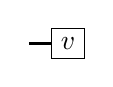
\begin{tikzpicture}[baseline=(current bounding box.center)]
    \node[draw] (s0) at (0,0) {$v$};
    \draw [thick] (-0.5,0)--(s0);
  \end{tikzpicture},
\end{equation}
其中$v=\begin{pmatrix} v_1 \\ v_2 \\ \vdots \\ v_n \end{pmatrix}$。
当给腿赋予指定的指标时,可以获得所表示向量的分量:
\begin{equation}
  \braket{i}{v}
  =v_i=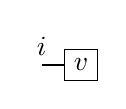
\begin{tikzpicture}
    \node[draw] (s0) at (0,0) {$v$};
    \draw [thick] (-0.5,0)--(s0);
    \node[above] at (-0.5,0) {$i$};
  \end{tikzpicture}
\end{equation}


矩阵在张量网络图中作为二阶张量,可以被表示为具有左右两侧连线的节点:
\begin{equation}
  A
  =
  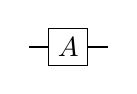
\begin{tikzpicture}[baseline=(current bounding box.center)]
    \node[draw] (s0) at (0,0) {$A$};
    \draw [thick] (-0.5,0)--(s0) (s0)--(0.5,0);
  \end{tikzpicture},
\end{equation}
其中$A=\begin{pmatrix} a_{11} & a_{12} \cdots \\ a_{21} & a_{22} \cdots \\ \vdots & \vdots \end{pmatrix}$。
矩阵的元素可通过指定连接的腿的指标获得:
\begin{equation}
  a_{ij}=
  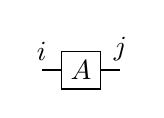
\begin{tikzpicture}[baseline=(current bounding box.center)]
    \node[draw] (s0) at (0,0) {$A$};
    \draw [thick] (-0.5,0)--(s0) (s0)--(0.5,0);
    \node[above] at (-0.5,0) {$i$};
    \node[above] at (0.5,0) {$j$};
  \end{tikzpicture}
\end{equation}


由矩阵的张量网络图表示,矩阵的转置操作可通过旋转张量对应的连接方向实现:
\begin{equation}\label{eq:tn:matrix_transpose}
  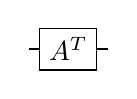
\begin{tikzpicture}[baseline=(current bounding box.center)]
    \node[draw] (s0) at (0,0) {$A^T$};
    \draw [thick] (-0.5,0)--(s0) (s0)--(0.5,0);
  \end{tikzpicture}
  =
  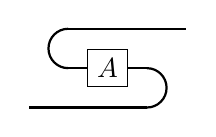
\begin{tikzpicture}[baseline=(current bounding box.center)]
    \node[draw] (s0) at (0,0) {$A$};
    \draw[thick] (-0.5,0)--(s0) (s0)--(0.5,0);
    \draw[thick] (-0.5,0.5) arc(90:270:0.25);
    \draw[thick] (0.5,-0.5) arc(-90:90:0.25);
    \draw[thick] (-0.5,0.5)--(1,0.5) (0.5,-0.5)--(-1,-0.5);
  \end{tikzpicture}
\end{equation}

对于矩阵的乘法操作,在张量网络图中是由连接相邻张量的对应边实现指标收缩来表示:
\begin{equation}\label{eq:tn:matrix_product}
  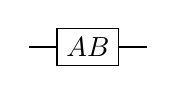
\begin{tikzpicture}[baseline=(current bounding box.center)]
    \node[draw] (s1) at (0,0) {$AB$};
    \draw [thick] (-0.75,0)--(s1) (s1)--(0.75,0);
  \end{tikzpicture}
  =
  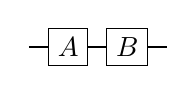
\begin{tikzpicture}[baseline=(current bounding box.center)]
    \node[draw] (s0) at (0,0) {$A$};
    \node[draw] (s1) at (0.75,0) {$B$};
    \draw [thick] (-0.5,0)--(s0) (s0)--(s1) (s1)--(1.25,0);
  \end{tikzpicture}
\end{equation}
这是因为矩阵乘法的元素表达式为
\begin{equation}
  (AB)_{ij}=\sum_k A_{ik}B_{kj}=\sum_k
  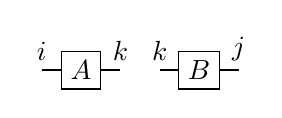
\begin{tikzpicture}[baseline=(current bounding box.center)]
    \node[draw] (s0) at (0,0) {$A$};
    \node[draw] (s1) at (1.5,0) {$B$};
    \draw [thick] (-0.5,0)--(s0) (s0)--(0.5,0) (s1)--(2,0) (s1)--(1,0);
    \node[above] at (-0.5,0) {$i$};
    \node[above] at (0.5,0) {$k$};
    \node[above] at (1,0) {$k$};
    \node[above] at (2,0) {$j$};
    \end{tikzpicture}=
    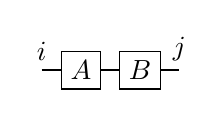
\begin{tikzpicture}[baseline=(current bounding box.center)]
        \node[draw] (s0) at (0,0) {$A$};
        \node[draw] (s1) at (0.75,0) {$B$};
        \draw [thick] (-0.5,0)--(s0) (s0)--(s1) (s1)--(1.25,0);
        \node[above] at (-0.5,0) {$i$};
        \node[above] at (1.25,0) {$j$};
    \end{tikzpicture}
\end{equation}





除了矩阵的乘法,另一种常见的张量积操作,在张量网络图中被表示为为张量的垂直堆叠:
\begin{equation}\label{eq:tn:tensor_product}
  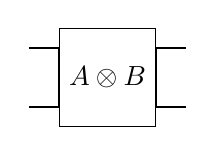
\begin{tikzpicture}[baseline=(current bounding box.center)]
    \node[draw,minimum height=1.25cm] (s1) at (0,0) {$A\otimes B$};
    \draw [thick] (-1,0.375)-|(s1.west) (-1,-0.375)-|(s1.west) (s1.east)|-(1,0.375) (s1.east)|-(1,-0.375);
  \end{tikzpicture}
  =
  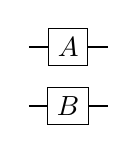
\begin{tikzpicture}[baseline=(current bounding box.center)]
    \node[draw] (s0) at (0,0) {$A$};
    \node[draw] (s1) at (0,-0.75) {$B$};
    \draw [thick] (-0.5,0)--(s0)--(0.5,0)  (-0.5,-0.75)--(s1)--(0.5,-0.75);
  \end{tikzpicture}
\end{equation}


矩阵的迹运算可以通过将张量的对应边连接并收缩来表示:
\begin{equation}\label{eq:tn:trace}
  \Tr{A}
  =
  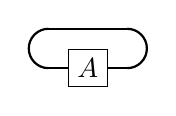
\begin{tikzpicture}[baseline=(current bounding box.center)]
    \node[draw] (s0) at (0,0) {$A$};
    \draw [thick] (-0.5,0)--(s0) (s0)--(0.5,0);
    \draw[thick] (-0.5,0.5) arc(90:270:0.25);
    \draw[thick] (0.5,0) arc(-90:90:0.25);
    \draw [thick] (-0.5,0.5)--(0.5,0.5);
  \end{tikzpicture}
\end{equation}

上述图记号通过几何拓扑直观反映了张量运算的代数结构,特别在处理高维张量收缩时,能有效降低传统指标记法的复杂性。后续章节将基于此记号体系,介绍Pauli路径积分算法的张量网络图表示。


\section{本章小结}
本章介绍了量子信息科学的基本概念,包括量子信息科学的研究背景、量子力学的基本知识、量子计算的基本概念等。介绍了表示量子系统状态的纯态、混合态、密度矩阵的概念,接着介绍了量子态的演化、量子测量的概念。最后介绍了量子计算的基本概念,包括量子比特、量子线路、量子门、量子噪声等。为了后续章节的讨论,还介绍了张量网络图的基本概念,作为一种直观的数学工具,将复杂的张量运算转化为可视化的图形操作。

在后面的章节中,我们将介绍
%#TODO
\chapter{Pauli路径积分}

\section{路径积分的定义}
s


%\chapter{具体线路的复杂度与误差分析}

\chapter{含噪的变分量子线路模拟}\label{chap:noisy_vqa}

\section{背景介绍}
在如今NISQ时代,噪声难以避免的出现在量子线路中。这些噪声导致许多需要高保真度的量子算法难以实现。比如Shor算法需要使用到深层量子线路,因此对噪声的容忍度较低,在现有超导量子处理器上(单比特门错误率$\~10^{-3}$,两比特门$\~10^{-2}$)保真度将指数衰减至可忽略水平,导致计算失效。

为了在近期的量子设备中实现实用性的量子算法,变分量子算法(Variational Quantum Algorithm,VQA)~\cite{Cerezo2021variational,mcclean2016theory,tilly2022variational}作为最受欢迎的一类NISQ算法,普遍被认为是一个很好的解决方案。
变分量子算法通过将量子电路的参数优化与经典优化器相结合,其核心思想基于变分原理:构造变分量子线路,以产生作为试探的量子态,通过经典优化器调整参数,使系统能量或目标函数达到极值。
通过这一"量子执行-经典反馈"的混合结构,变分量子算法展示出独特的噪声适应性:仅仅依靠浅层量子线路(通常$<100$层)因此能够将噪声的积累限制在可以控制的范围内。

基于变分量子算法发展的一系列算法,已经在各个领域产生了广泛的应用:
在组合优化领域,量子近似优化算法~\cite{farhi2014quantum,moll2018quantum}(Quantum Approximate Optimization Algorithm,QAOA)通过将目标优化问题编码为物理系统的基态求解问题,通过交替应用混合哈密顿量和问题哈密顿量的演化来逼近基态能量。
在量子化学领域,变分量子本征求解器~\cite{peruzzo2014variational, kandala2017hardwarea,li2022toward}(Variational Quantum Eigensolver,VQE)通过变分量子线路模拟分子哈密顿量的基态能量,从而实现分子结构的计算。
在量子机器学习领域,量子支持向量机~\cite{havlivcek2019supervised}(Quantum Support Vector Machine,QSVM)通过变分量子线路实现量子数据的分类,以及量子神经网络~\cite{beer2020training,huang2021experimental, mitarai2018quantum}(Quantum Neural Network,QNN)通过变分量子线路实现量子数据的学习。
在量子纠错领域,基于变分的量子纠错~\cite{johnson2017qvector,xu2021variational}通过变分量子线路实现量子纠错码的编码和解码。


虽然变分量子算法作为NISQ时代最有希望的候选者,并且已经开发了一系列的应用,但是在实际应用中,是否能在NISQ设备中利用变分量子算法产生实际的量子优势仍然是一个开放的问题。其中一个主要的挑战是变分量子算法的鲁棒性:在NISQ设备中,由于噪声的存在,变分量子算法的性能会受到严重影响。为了研究噪声下变分量子算法的优势,我们将通过OBPPP算法对其进行模拟,研究其产生量子优势的条件。


在本节的讨论中,我们将变分量子线路的深度记为 $L$,即 $\mathcal{U}(\bm{\theta})=\mathcal{U}_L(\bm{\theta}_L)\cdots\mathcal{U}_1(\bm{\theta}_1)$。变分量子线路的每一层 $\mathcal{U}_i(\bm{\theta}_i)$ 是由 $R_i$ 个旋转门和 $C_i$ 个 Clifford 门组成,这些门作用于相互不相交的量子比特上,$\bm{\theta}_i=(\theta_{i,1},\cdots,\theta_{i,R_i})$ 表示第 $i$ 层的参数向量,$\bm{\theta}=(\bm{\theta}_1,\cdots,\bm{\theta}_L)$ 表示整个变分量子线路的参数向量。
具体来说,第 $i$ 层中的第 $j$ 个旋转门表示为 $U_{i, j}(\theta_{i,j})=\exp{-i \frac{\theta_{i,j}}{2} \sigma_{i,j}}$,其中 $j \in \{1, \cdots , R_i\}$,$\theta_{i,j}$ 是旋转角度,$\sigma_{i, j}\in \{\mathbb{I}, X,Y,Z\}^{\otimes n}$为Pauli旋转门对应的Pauli算符。
类似地,第 $i$ 层中的第 $k$ 个 Clifford 门表示为 $V_{i,k}$,其中 $k \in \{1, \cdots , C_i\}$。$V_{i,k}\in\{\mathrm{H}(a),\mathrm{S}(a),\mathrm{CNOT}(a,b)\}$,其中 $a,b $ 指的是门作用的量子比特的序号。

记所有Pauli旋转门 $U_{i,j}(\theta_{i,j})$ 的 Pauli 算符集合为 $\{\sigma_{i,j}\}$。
我们将集合 $\{\overline{\sigma}_{i,j}\}$ 表示为经过后续 Clifford 门变换后的所有 $\sigma_{i,j}$,即 $\overline{\sigma}_{i,j}= \mathcal{V}_{L} \cdots \mathcal{V}_{i} \sigma_{i,j} \mathcal{V}_{i}^\dagger \cdots \mathcal{V}_{L}^\dagger$,其中 $\mathcal{V}_{i} = \prod_{k=1}^{C_i} V_{i,k}$ 是对应于第 $i$ 层中所有 Clifford 门的张量积的幺正变换。

为了确保引理~\ref{lemma:cross_items} 的有效性,我们需要一个容易实现的前提条件:假设集合 $\{\overline{\sigma}_{i,j}\}$ 在忽略相位的意义下,可以生成 $\{\mathbb{I}, X, Y, Z\}^{\otimes n}$。这一条件可以通过以下等式来表示:
\begin{equation}\label{eq:generate}
  \langle \{\overline{\sigma}_{i,j}\}\rangle/\left(\langle \{\overline{\sigma}_{i,j}\}\rangle\cap\langle i\mathbb{I}^{\otimes n}\rangle\right)=\{\mathbb{I},X,Y,Z\}^{\otimes n},
\end{equation}
这里 $\langle \{\overline{\sigma}_{i,j}\} \rangle$ 指的是由集合 $\{\overline{\sigma}_{i,j}\}$ 生成的 Pauli 子群,这意味着 $\langle \{\overline{\sigma}_{i,j}\}\rangle$ 中的元素可以表示为 $\{\overline{\sigma}_{i,j}\}$ 中元素的有限乘积。
为了证明这一条件确实容易满足,考虑在电路的最后两层中,每个量子比特上都有一层 $R_X$ 门和一层 $R_Z$ 门作用,那么 $\{X_i, Z_i\}_{i=1,\cdots,n}$ 包含在 $\{\overline{\sigma}_{i,j}\}$ 中。这些 $\{ X_i,Z_i \}_{i=1,\cdots,n}$ 足以生成 $\{\mathbb{I},X,Y,Z\}^{\otimes n}$。事实上,这一充分条件可以进一步减弱,如第~\ref{temp:subsubsection:cross_items}节 中所示。


\section{计算复杂度分析}

在本节中,我们将估计使用OBPPP算法模拟含噪声变分量子线路的计算复杂度。根据式~\eqref{eq:total_cost}我们可以看到,计算$\widehat{\langle O \rangle}$的时间复杂度可以表示为$C = C_s+N_MC_f$,其中$C_s$是枚举所有满足条件的Pauli路径的时间复杂度,$N_M$是满足条件的Pauli路径的数量,$C_f$是计算每个Pauli路径的贡献的时间复杂度。
其中$C_f$可以进一步分解为$C_{f\mathcal{U}}+C_{fO}+C_{f\rho}$,其中$C_{f\mathcal{U}}$是计算与中间量子门关联的项$\prod\Tr{s_i\mathcal{U}_i s_{i-1}\mathcal{U}_i^\dagger}$的时间复杂度,$C_{fO}$是和观测量相关的$\Tr{Os_L}$项的时间复杂度,$C_{f\rho}$是和初态相关的$\Tr{\rho s_0}$项的时间复杂度。

对于空间复杂度,根据式~\eqref{eq:space_cost},我们可以得到$S = S_s+S_f$,其中$S_s$是枚举所有满足条件的Pauli路径的空间复杂度,$S_f$是计算每个Pauli路径的贡献函数的空间复杂度。根据式~\eqref{eq:space_f},$S_f$可以进一步分解为$\max\{S_{f\mathcal{U}},S_{fO},S_{f\rho}\}$,其中$S_{f\mathcal{U}}$是计算与中间量子门关联的项$\prod\Tr{s_i\mathcal{U}_i s_{i-1}\mathcal{U}_i^\dagger}$的空间复杂度,$S_{fO}$是和观测量相关的$\Tr{Os_L}$项的空间复杂度,$S_{f\rho}$是和初态相关的$\Tr{\rho s_0}$项的空间复杂度。

在第~\ref{sec:obppp}节中,我们已经讨论了枚举所有满足条件的Pauli路径的时间复杂度$C_s$和空间复杂度$S_s$,以及在设定稀疏性条件下$C_{fO}$、$C_{f\rho}$和$S_{fO}$、$S_{f\rho}$的估计。
在本节中,我们将讨论对于变分量子线路$C_{f\mathcal{U}}$和$S_{f\mathcal{U}}$的估计,以及式~\eqref{eq:case1:cost_s}\eqref{eq:case1:N_M}\eqref{eq:case2:cost_s}\eqref{eq:case2:N_M}\eqref{eq:path:space_cost}中关联的$N_{\text{max}}$、$C_{\text{split}}$和$S_{\text{split}}$的估计。


为了估计$C_{f\mathcal{U}}$和$S_{f\mathcal{U}}$我们首先介绍以下命题:
\begin{proposition}\label{prop:layer_terms}
    计算 $f$ 中第 $i$ 层项的时间和空间复杂度为 $\order{n}$,可通过如下等式计算:
    \begin{equation}\label{eq:i-layer_terms}
    \begin{aligned}
    \Tr{s_i\mathcal{U}_i s_{i-1}\mathcal{U}_i^\dagger}&=\Tr{\left(s_i s_{i-1}\right)\big|_{I_i}}\\
    \prod_{k=1}^{C_i}&\Tr{\left(s_iV_{i,k} s_{i-1}V_{i,k}^{\dagger}\right)\big|_\g{V_{i,k}}}\prod_{\sigma_{i,j}\in C(i,s_{i-1})}\Tr{\left(s_i s_{i-1}\right)\big|_\g{\sigma_{i,j}}}\\
    \prod_{\sigma_{i,j'}\in AC(i,s_{i-1})} &\Bigg\{ \Tr{\left(s_i s_{i-1}\right)\big|_\g{\sigma_{i,j'}}}\cos{\theta_{i,j'}}- \Tr{\left(is_i \sigma_{i,j'}s_{i-1}\right)\big|_\g{\sigma_{i,j'}}}\sin{\theta_{i,j'}}  \Bigg\},
    \end{aligned}
    \end{equation}
    其中$\supp:\{\mathbb{I}, X, Y, Z\}^{\otimes n}\cup\{\mathrm{CNOT}_{a,b},\mathrm{H}_a,\mathrm{S}_a\}\rightarrow2^{\{1,\cdots, n\}}$ 为从幺正算符到其非平凡作用的量子比特的映射。这里 $2^{\{1,\cdots, n\}}$ 表示 $\{1,\cdots, n\}$ 的所有子集。
    为了简化,我们将 $i$ 层中 $n$ 个量子比特的索引根据所应用门的类型分为三组。这些组分别表示为符号 $\big|_{I_i}$、$\big|_\g{V_{i,k}}$ 和 $\big|_\g{\sigma_{i,j}}$,对应于没有门作用、Clifford 门作用和 Pauli 旋转门作用。此外,集合 $C(i,s_{i-1})$ 和 $AC(i,s_{i-1})$ 分别表示 $\{\sigma_{i,j}\}_{j=1}^{R_i}$ 中与 $s_{i-1}$ 对易和反对易的 Pauli 算符集合。
\end{proposition}

\begin{proof}
    
    在变分量子线路中,$\mathcal{U}_i$ 由一系列门 $U_{i,1},\cdots,U_{i,R_i}$ 和 $V_{i,1},\cdots,V_{i,C_i}$ 组成,并且不会在每个量子比特上操作两次。
    Pauli 旋转门 $U_{i,j}(\theta_{i,j})$ 的形式为:
    \begin{equation}
      U_{i,j}(\theta_{i,j})=\exp{-i \frac{\theta_{i,j}}{2} \sigma_{i,j}}.
    \end{equation}
    
    Clifford 门 $V_{i,k}$ 可以从 $\{\mathrm{H}(a),\mathrm{S}(a),\mathrm{CNOT}(a,b) \}_ {a\neq b}$ 中选择。
    因此,我们有:
    \begin{equation}
      \begin{aligned}
        \Tr{s_i\mathcal{U}_i s_{i-1}\mathcal{U}_i^\dagger}=&\Tr{\left(s_i s_{i-1}\right)\big|_{I_i}}
        \prod_{k=1}^{C_i}\Tr{\left(s_iV_{i,k} s_{i-1}V_{i,k}^{\dagger}\right)\big|_\g{V_{i,k}}}\\
        &\prod_{j=1}^{R_i}\Tr{\left(s_i U_{i,j}(\theta_{i,j}) s_{i-1} U_{i,j}^\dagger(\theta_{i,j})\right) \big|_\g{\sigma_{i,j}}}.
      \end{aligned}
    \end{equation}
    
    厄米 算符 $X$ 的指数定义为 $\exp{X}=\sum_{k=0}^\infty\frac{X^k}{k!}$。对于 Pauli 算符,任何 Pauli 算符号的满足自反性 $\sigma^2=\mathbb{I}$,因此我们有:
    \begin{equation}
      \exp{-i \frac{\theta}{2} \sigma}=\sum_{k=0}^\infty\frac{(-i \frac{\theta}{2}\sigma)^k}{k!}=\sum_{k=0}^\infty\frac{(-1)^k (\frac{\theta}{2})^{2k}}{(2k)!} \mathbb{I}- i\frac{(-1)^k (\frac{\theta}{2})^{2k+1}}{(2k+1)!}\sigma=\cos{\frac{\theta}{2}}\mathbb{I}-i \sin{\frac{\theta}{2}}\sigma.
    \end{equation}
    
    根据 Pauli算符$\sigma$ 和另一个 Pauli算符 $\sigma'$ 的对易/反对易关系,有:
    \begin{equation}
    \begin{aligned}
    &\sigma'\exp{-i \frac{\theta}{2} \sigma}=\exp{-i \frac{\theta}{2} \sigma}\sigma',\text{ 如果 }\sigma\text{ 与 }\sigma'\text{ 对易。}\\
    &\sigma'\exp{-i \frac{\theta}{2} \sigma}=\exp{i \frac{\theta}{2} \sigma}\sigma',\text{ 如果 }\sigma\text{ 与 }\sigma'\text{ 反对易。}\\
    \end{aligned}
    \end{equation}
    因此可以将 $\{\sigma_{i,j}\}$ 分为两种情况。如果 $\sigma_{i,j}$ 与 $s_{i-1}$ 对易,有:
    
    \begin{equation}
      \begin{aligned}
      \Tr{\left(s_i U_{i,j}(\theta_{i,j}) s_{i-1} U_{i,j}^\dagger(\theta_{i,j})\right)\big|_\g{\sigma_{i,j}}}
      &=\Tr{(s_i \exp{-i \frac{\theta_{i,j}}{2}\sigma_{i,j} }  \exp{i \frac{\theta_{i,j}}{2}\sigma_{i,j} }s_{i-1}) \big|_\g{\sigma_{i,j}}}\\
      &=\Tr{(s_i \exp{-i \frac{\theta_{i,j}}{2}\sigma_{i,j} } \exp{i \frac{\theta_{i,j}}{2}\sigma_{i,j} }s_{i-1}) \big|_{\g{\sigma_{i,j}}}}\\
      &=\Tr{(s_i s_{i-1})\big|_{\g{\sigma_{i,j}}}}.
    \end{aligned}
    \end{equation}
    而若 $\sigma_{i,j}$ 与 $s_{i-1}$ 反对易,则有:
    \begin{equation}
      \begin{aligned}
      &\Tr{\left(s_i U_{i,j}(\theta_{i,j}) s_{i-1} U_{i,j}^\dagger(\theta_{i,j})\right)\big|_\g{\sigma_{i,j}}}\\
      &=\Tr{ \left(s_i\exp{-i \frac{\theta_{i,j}}{2}\sigma_{i,j} } s_{i-1}\exp{i \frac{\theta_{i,j}}{2}\sigma_{i,j}}\right) \big|_\g{\sigma_{i,j}}}\\
      &=\Tr{\left( s_i  \exp{-i\theta_{i,j}\sigma_{i,j}} s_{i-1}\right) \big|_\g{\sigma_{i,j}}}\\
      &=\Tr{ \left(s_i (\cos{\theta_{i,j}}\mathbb{I}-i\sin{\theta_{i,j}}\sigma_{i,j}) s_{i-1} \right) \big|_\g{\sigma_{i,j}}}\\
      &=\Tr{\left(s_i s_{i-1}\right)\big|_\g{\sigma_{i,j}}}\cos{\theta_{i,j}}-\Tr{\left(i s_i \sigma_{i,j}s_{i-1}\right)\big|_\g{\sigma_{i,j}}}\sin{\theta_{i,j}}.
    \end{aligned}
    \end{equation}
    以上完成了 式.~\eqref{eq:i-layer_terms} 的证明。

    此外,对于计算复杂度,可以分类讨论。
    对$\big|_{I_i}$项,需要比较$s_i$ 和 $s_{i-1}$ 在$\supp(I_i)$上是否相同。这一操作的时间和空间复杂度为 $\order{n}$。
    对于$\big|_\g{V_{i,k}}$项,需要比较$s_i$ 和 $V_{i,k}s_{i-1}V_{i,k}^\dagger$ 在$\supp(V_{i,k})$上是否相同,因为 $V_{i,k}\in\{\mathrm{H}(a),\mathrm{S}(a),\mathrm{CNOT}(a,b)\}$,$V_{i,k}s_{i-1}V_{i,k}^\dagger$ 可以在 $\order{1}$ 的时间内计算。因此,对于所有$\big|_\g{V_{i,k}}$项,总的时间和空间复杂度为 $\order{n}$。
    对于$\big|_\g{\sigma_{i,j}}$项,需要首先比较$s_{i-1}$ 和 $\sigma_{i,j}$ 在$\supp(\sigma_{i,j})$上的对易关系,然后再比较$s_i$ 和 $s_{i-1}$(或是$\sigma_{i,j'}s_{i-1}$) 在$\supp(\sigma_{i,j})$上是否相同。这两个操作的时间和空间复杂度为均为 $\order{\abs{\supp(\sigma_{i,j})}}$。因此,对于所有$\big|_\g{\sigma_{i,j}}$项,总的时间和空间复杂度为 $\order{n}$。

    综上所述,计算 $f$ 中第 $i$ 层项的时间和空间复杂度为 $\order{n}$。
    \end{proof}


\begin{remark}\label{remark:f_ele}
通过利用不同 Pauli 算符的正交性,可以在 $\Tr{s_i\mathcal{U}_i s_{i-1}\mathcal{U}_i^\dagger} \neq 0$ 时,建立以下$s_i$ 和 $s_{i-1}$ 之间的关系:

\begin{tabular}{|c|c|c|}
  \hline
   项 & 关系 & $f$ 中的因子\\
  \hline
  ${I_i}$ &$s_{i-1}\big|_{I_i} = s_{i}\big|_{I_i}$& 1 \\
  \hline
  $V_{i,k}$ &$s_{i-1}\big|_\g{V_{i,k}}= \pm V_{i,k}^{\dagger} s_{i}V_{i,k}\big|_\g{V_{i,k}}$& $\pm 1$ \\
  \hline
  $C(i,s_{i-1})=C(i,s_{i})$&$s_{i}|_\g{\sigma_{i,j}}=s_{i-1}|_\g{\sigma_{i,j}}$& 1 \\
  \hline
  \multirow{2}{*}{$AC(i,s_{i-1})=AC(i,s_{i})$}
  &$s_{i}|_\g{\sigma_{i,j}}=s_{i-1}|_\g{\sigma_{i,j}}$& $\cos{\theta_{i,j}}$ \\
  \cline{2-3}
  &$s_{i}|_\g{\sigma_{i,j}}=\pm i \sigma_{i,j} s_{i-1}|_\g{\sigma_{i,j}}$& $\mp \sin{\theta_{i,j}}$ \\
  \hline
\end{tabular}

以上表格中的关系可以帮助我们计算 $f$ 中的每一项。以$I_i$ 为例,该表格表面若$\bm{s}$有非平凡贡献$f(\mathcal{U},\bm{s},O,\rho) \neq 0$,则必有$s_{i-1}\big|_{I_i} = s_{i}\big|_{I_i}$。这意味着 $s_{i-1}$ 和 $s_{i}$ 在第 $i$ 层的第 $j$ 个旋转门上的作用是相同的。且这一关系为$f$带来了一个因子1。

通过命题~\ref{prop:layer_terms},可以得知对于变分量子线路中的每一层,计算 $f$ 中的每一项的时间和空间复杂度为 $\order{n}$。因此,计算 $f$ 中的所有项的时间复杂度为 $\order{L n}$,得到式~\eqref{eq:cost_f}中$C_{f\mathcal{U}}=\order{L n}$。式~\eqref{eq:space_f}中的$S_{f\mathcal{U}}=\order{n}$。
\end{remark}

结合式~\eqref{eq:cost_rho}和式~\eqref{eq:cost_O},我们可以得到式~\eqref{eq:cost_f}对于变分量子线路取值为:
\begin{equation}\label{eq:vqa:c_f}
    C_f=\order{L n}+\order{n}+\order{\poly(n)}=\order{\poly(n)+L n}.
\end{equation}
式~\eqref{eq:space_f}对于变分量子线路取值为:
\begin{equation}
    S_f=\max\{\order{n},\order{\poly(n)},\order{\poly(n)}\}=\order{\poly(n)}.
\end{equation}


在OBPPP算法的复杂度的分析中,还涉及到对一个给定的Pauli算符$s$和构成线路$\mathcal{U}$的门集合$\{U_{i,j}\}$,求解以下集合:
\begin{equation}
    \left\{ s'\mid \Tr{s' U^\dagger_{i,j}s U_{i,j}}\neq 0 \right\}.
\end{equation}
为了估计整个算法的时间复杂度,我们需要考虑这一集合的最大元素数$N_{\text{max}}$、求解该集合所需要的时间$C_{\text{split}}$和空间复杂度$S_{\text{split}}$。

对于在变分线路中,每个门可最大分裂的Pauli 算符数量$N_{\max}$:
\begin{equation}
    N_{\text{max}} = \max_{i,j,s}\abs{ \left\{ s'\mid \Tr{s' U^\dagger_{i,j}s U_{i,j}}\neq 0 \right\}}.
\end{equation}
注意到,当 $U_{i,j}$ 为Clifford 门时,因为Clifford 门作用于Pauli 算符后仍为Pauli 算符,因此Clifford门不会增加Pauli 算符的数量。而当 $U_{i,j}$ 为Pauli 旋转门时,假设旋转的Pauli算符为$\sigma$。根据注释~\ref{remark:f_ele}当$s$与$\sigma$对易时,$s'=s$,因此最大分裂个数为1。当$s$与$\sigma$反对易时,$s'=s$ 或 $s'=\pm i \sigma s$,因此最大分裂个数为2。因此,$N_{\text{max}}=2$。

对于求解该集合所需要的时间$C_{\text{split}}$和空间复杂度$S_{\text{split}}$,对于Clifford门可以以$\order{1}$的时间和空间复杂度求解。对于Pauli 旋转门,需要比较$s$和$s'$的对易关系,并输出$s'$。这一操作的时间和空间复杂度为 $\order{n}$。因此,$C_{\text{split}}=\order{n}$,$S_{\text{split}}=\order{n}$。

因此,对于变分量子线路,对于\textbf{情况1}根据式~\eqref{eq:case1:N_M}和式~\eqref{eq:case1:cost_s},Pauli路径枚举过程的时间复杂度为:
\begin{equation}
    C_{s}=\mathrm{Poly}(n) \order{L} C_{\text{split}} N_{\text{max}}^{M}= \mathrm{Poly}(n) \order{L} 2^M.
\end{equation}
满足$\abs{\bm{s}}\leq M$的Pauli路径数量最多为:
\begin{equation}\label{eq:vqa:case1:N_M}
    N_M=\poly(n) N_{\text{max}}^{M}=\poly(n) 2^M.
\end{equation}


对于\textbf{情况2},我们需要首先说明,对于变分量子线路是自然满足定义~\ref{def:monotonic}中刻画的对噪声关联的Hamming Weight 单调增条件。即对量子线路$\mathcal{U}$中的任意门$U_{i,j}$有$\abs{\left\{s'\mid \Tr{sU_{i,j}s' U_{i,j}^\dagger}\neq 0,\ \abs{s'}_{\mathcal{N}}=0\right\}}\leq 1$,其中$s$和$s'$是Pauli算符。
当$U_{i,j}$为Clifford门时,对给定的$s$因为满足$\Tr{sU_{i,j}s' U_{i,j}^\dagger}\neq 0$的只有一个,因此$\abs{\left\{s'\mid \Tr{sU_{i,j}s' U_{i,j}^\dagger}\neq 0,\ \abs{s'}_{\mathcal{N}}=0\right\}}\leq 1$自然成立。
当$U_{i,j}$为Pauli旋转门时,不妨设为$U_{i,j}(\theta_{i,j})=\exp{-i \frac{\theta_{i,j}}{2} \sigma_{i,j}}$。根据注释~\ref{remark:f_ele},若$s$与$\sigma_{i,j}$对易,则只有$s'=s$满足$\Tr{sU_{i,j}s' U_{i,j}^\dagger}\neq 0$。若$s$与$\sigma_{i,j}$反对易,则只有$s'=s$或$s'=\pm i \sigma_{i,j}s$满足$\Tr{sU_{i,j}s' U_{i,j}^\dagger}\neq 0$。不失一般性,可假设$\abs{\bullet}_{\mathcal{N}}=\abs{\bullet}_Y+\abs{\bullet}_Z$,即$\mathcal{N}$的噪声模型只包含$X$的Pauli算符。因此,若$\abs{s}_{\mathcal{N}}=0$则必有$\abs{\pm i \sigma_{i,j}s}_{\mathcal{N}}\neq 0$,因为$s$与$\sigma_{i,j}s$反对易,反之亦然。因此,对于变分量子线路,满足对噪声关联的Hamming Weight 单调增条件。


对于\textbf{情况2},根据式~\eqref{eq:case2:N_M}和式~\eqref{eq:case2:cost_s},当量子线路$\mathcal{U}$满足对噪声关联的Hamming Weight 单调增时,Pauli路径枚举过程的时间复杂度为:
\begin{equation}
    C_{s}=\mathrm{Poly}(n) \order{(nL)^M} C_{\text{split}} N_{\text{max}}^{M}= \mathrm{Poly}(n) \order{(nL)^M} 2^M.
\end{equation}\label{eq:vqa:case2:N_M}
满足$\abs{\bm{s}}\leq M$的Pauli路径数量最多为:
\begin{equation}
    N_M=\poly(n)(nLN_{\text{max}})^{M+1}= \poly(n)(2nL)^{M+1}.
\end{equation}

对于枚举过程的空间复杂度,根据式~\eqref{eq:path:space_cost}:
\begin{equation}
    S_{s}=\order{\mathrm{Poly}(n)+\max\{S_{\text{split}},n\}L}=\order{\mathrm{Poly}(n)+nL}.
\end{equation}


综上所述,对于变分量子线路,根据式~\eqref{eq:total_cost}和式~\eqref{eq:space_cost},在给定截断参数$M$的情况下,含噪声期望值模拟的时间复杂度$C$和空间复杂度$S$分别为:
\begin{equation}\label{eq:vqa:cost}
    \begin{aligned}
        C&=\begin{cases}
            \mathrm{Poly}(n) \order{L} 2^M, & \text{如果$\abs{\bullet}_{\mathcal{N}}$属于\textbf{情况1}} \\
           \mathrm{Poly}(n) \order{(2nL)^{M+1}}, & \text{如果$\abs{\bullet}_{\mathcal{N}}$属于\textbf{情况2}}
        \end{cases}\\
        S&=\mathrm{Poly}(n)+nL,
    \end{aligned}
\end{equation}
其中$n$为量子比特数,$L$为线路深度,$\mathcal{N}$为噪声模型。


\section{误差分析}
在上一节中,已经得到了在给定截断参数$M$的情况下,模拟变分量子线路的计算复杂度(式~\eqref{eq:vqa:cost})。在这一节中,我们将讨论在给定的误差容忍度$\epsilon$下,如何选择截断参数$M$。

误差可以用均方误差(Mean Square Error, MSE)来衡量,对于一个随机变量$X$,其均方误差定义为$\mathbb{E}[(X-\hat{X})^2]$,其中$\hat{X}$是$X$的估计值。在这里,我们考虑的是含噪声期望值模拟的误差,即真实含噪声期望值$\widetilde{\langle O\rangle}$和其估计值$\widehat{\langle O\rangle}$之间的均方误差。根据定义(式~\eqref{eq:noise_expectation}和式~\eqref{eq:truncated_expectation}),含噪声期望值模拟的误差为:
\begin{equation}
    \widetilde{\langle O\rangle}-\widehat{\langle O\rangle}=\sum_{\abs{\bm{s}}_{\mathcal{N}}>M}f(\widetilde{\mathcal{U}},\bm{s},O,\rho),
\end{equation}
其中$\abs{\bullet}_{\mathcal{N}}$定义在式~\eqref{eq:noise_hamming_weight}中,表示与噪声模型$\mathcal{N}$关联的Hamming weight,$f(\widetilde{\mathcal{U}},\bm{s},O,\rho)$定义在式~\eqref{eq:noise_contribution}中,表示一个Pauli路径$\bm{s}$对含噪声期望值的贡献。


如果有式~\eqref{eq:generate}成立,有以下引理成立:
\begin{lemma}\label{lemma:cross_items}
    对于变分量子线路,如果式~\eqref{eq:generate}成立,则对任意两个不同的Pauli路径$\bm{s}$和$\bm{s}'$,有:
    \begin{equation}\label{eq:E_cross_equals_0}
        \mathbb{E}_{\bm{\theta}}\left[f(\widetilde{\mathcal{U}},\bm{s},O,\rho)f(\widetilde{\mathcal{U}},\bm{s}',O,\rho)\right]=0,
    \end{equation}
    其中期望是对于均匀随机选择的旋转角度$\bm{\theta}$。
\end{lemma}
我们先暂时跳过该引理的证明,我们将在后文中证明该引理。

关于均方误差,有以下引理:
\begin{lemma}\label{lemma:MSE_l}
    对于变分量子线路,如果式~\eqref{eq:E_cross_equals_0}成立,那么对任意的$\nu > 0$,只要截断参数$M$满足:
    \begin{equation}
        M\geq\frac{1}{4\gamma}\ln{\frac{\norm{O}_\infty^2}{\nu}},
    \end{equation}
    其中$\gamma:=\min\{p|{p \in \{p_x,p_y,p_z\},p\neq 0}\}$,那么含噪声期望值模拟的均方误差满足:
    \begin{equation}
        \mathbb{E}_{\bm{\theta}}\left[\left(\widetilde{\langle O\rangle}-\widehat{\langle O\rangle}\right)^2\right]\leq\nu,
    \end{equation}
    其中期望是对于均匀随机选择的旋转角度$\bm{\theta}$。
\end{lemma}
\begin{proof}
    根据式~\eqref{eq:noise_contribution},含噪声期望值模拟的误差为:
    \begin{equation}
        \widetilde{\langle O\rangle}-\widehat{\langle O\rangle}=\sum_{\abs{\bm{s}}_{\mathcal{N}}>M}f(\widetilde{\mathcal{U}},\bm{s},O,\rho).
    \end{equation}
    因此,含噪声期望值模拟的均方误差为:
    \begin{equation}
        \begin{aligned}
            \mathbb{E}_{\bm{\theta}}\left[\left(\widetilde{\langle O\rangle}-\widehat{\langle O\rangle}\right)^2\right]&=\mathbb{E}_{\bm{\theta}}\left[\left(\sum_{\abs{\bm{s}}_{\mathcal{N}}>M}f(\widetilde{\mathcal{U}},\bm{s},O,\rho)\right)^2\right]\\
            &=\sum_{\abs{\bm{s}}_{\mathcal{N}}>M}\mathbb{E}_{\bm{\theta}}\left[f(\widetilde{\mathcal{U}},\bm{s},O,\rho)^2\right],
        \end{aligned}
    \end{equation}
    其中,等号是因为根据式~\eqref{eq:E_cross_equals_0},对于任意两个不同的Pauli路径$\bm{s}$和$\bm{s}'$,有:
    \begin{equation}
        \mathbb{E}_{\bm{\theta}}\left[f(\widetilde{\mathcal{U}},\bm{s},O,\rho)f(\widetilde{\mathcal{U}},\bm{s}',O,\rho)\right]=0.
    \end{equation}
    
    另一方面,在无噪声的理想情况下,有:
    \begin{equation}
        \abs{\sum_{\bm{s}}f(\mathcal{U},\bm{s},O,\rho)}=\abs{\Tr{\rho \mathcal{U}^\dagger s \mathcal{U} O}}\leq\norm{O}_\infty.
    \end{equation}
    因此,有如下不等式:
    \begin{equation}
        \mathbb{E}_{\bm{\theta}}\left[ \sum_{\bm{s}}f(\widetilde{\mathcal{U}},\bm{s},O,\rho)\right]^2=\sum_{\bm{s}}\mathbb{E}_{\bm{\theta}}\left[f(\mathcal{U},\bm{s},O,\rho)^2\right]\leq\norm{O}_\infty^2.
    \end{equation}
    根据不等式~\eqref{eq:noise_suppression},可以得到:
    \begin{equation}\label{temp:eq:noise_suppression}
        \begin{aligned}
            \sum_{\abs{\bm{s}}_{\mathcal{N}}>M}\mathbb{E}_{\bm{\theta}}\left[f(\widetilde{\mathcal{U}},\bm{s},O,\rho)^2\right] &\leq (1-2\gamma)^{2M} \sum_{\abs{\bm{s}}_{\mathcal{N}}>M}\mathbb{E}_{\bm{\theta}}\left[f(\mathcal{U},\bm{s},O,\rho)^2\right]\\
            &\leq (1-2\gamma)^{2M} \norm{O}_\infty^2\\
            &\leq \exp{-4\gamma M} \norm{O}_\infty^2.
        \end{aligned}
    \end{equation}

    于是,对于任意的$\nu > 0$,只要截断参数$M$满足:
    \begin{equation}
        M\geq\frac{1}{4\gamma}\ln{\frac{\norm{O}_\infty^2}{\nu}},
    \end{equation}
    就有:
    \begin{equation}
        \mathbb{E}_{\bm{\theta}}\left[\left(\widetilde{\langle O\rangle}-\widehat{\langle O\rangle}\right)^2\right]\leq\nu.
    \end{equation}
\end{proof}
\begin{remark}
    特别的,对于退极化噪声模型,有$p_x=p_y=p_z=\frac{\lambda}{4}$,因此根据引理~\ref{lemma:noise},可以得到:
    \begin{equation}
        f(\widetilde{\mathcal{U}},\bm{s},O,\rho)=(1-\lambda)^{\abs{\bm{s}}}f(\mathcal{U},\bm{s},O,\rho).
    \end{equation}
    类似于式~\eqref{temp:eq:noise_suppression},可以得到:
    \begin{equation}
        \mathbb{E}_{\bm{\theta}}\left[\left(\widetilde{\langle O\rangle}-\widehat{\langle O\rangle}\right)^2\right] \leq (1-\lambda)^{2M} \norm{O}_\infty^2 \leq \exp{-2\lambda M} \norm{O}_\infty^2.
    \end{equation}
    因此,对于退极化噪声模型,只要截断参数$M$满足:
    \begin{equation}\label{eq:depolarizing_M:1}
        M\geq\frac{1}{2\lambda}\ln{\frac{\norm{O}_\infty^2}{\nu}},
    \end{equation}
    就有$\mathbb{E}_{\bm{\theta}}\left[\left(\widetilde{\langle O\rangle}-\widehat{\langle O\rangle}\right)^2\right]\leq\nu$。
\end{remark}

结合以上误差分析,以及过去的计算复杂度分析(式~\eqref{eq:vqa:cost}),我们可以得到如下推论:

\begin{corollary}\label{corollary:noise}
    对于变分量子线路,如果初始态密度矩阵$\rho$和观测量$O$分别满足稀疏性和Pauli稀疏性,且式~\eqref{eq:E_cross_equals_0}成立,那么对于任意的$\nu > 0$,则对于噪声\textbf{情况1},以多项式时间复杂度$\poly(n)\order{L}\left(\frac{\norm{O}_\infty}{\sqrt{\nu}}\right)^{\order{\frac{1}{\gamma}}}=\poly(n,L,\frac{1}{\sqrt{\nu}},\norm{O}_\infty)$;对于噪声\textbf{情况2},以准多项式时间复杂度$\poly(n)\order{(2nL)^{\ln \frac{\norm{O}_\infty}{\sqrt{\nu}}}}^{\order{\frac{1}{\gamma}}}$,能模拟含噪声期望值$\widetilde{\langle O\rangle}$且均方误差满足$\mathbb{E}_{\bm{\theta}}\left[\left(\widetilde{\langle O\rangle}-\widehat{\langle O\rangle}\right)^2\right]\leq\nu$。空间复杂度为$\order{\mathrm{Poly}(n)+nL}$。其中$\gamma:=\min\{p|{p \in \{p_x,p_y,p_z\},p\neq 0}\}$,$n$为量子比特数,$L$为线路深度。
\end{corollary}

结合Markov不等式,可以得到如下主要定理:
\begin{theorem}\label{thm:main}
    对于变分量子线路,如果初始态密度矩阵$\rho$和观测量$O$分别满足稀疏性和Pauli稀疏性,且式~\eqref{eq:E_cross_equals_0}成立,对于固定的$\gamma:=\min\{p|{p \in \{p_x,p_y,p_z\},p\neq 0}\}$,给定任意截断误差$\varepsilon$,存在一个多项式规模的经典算法来近似含噪声期望值$\widetilde{\langle O\rangle}$,在旋转角度$\bm{\theta}$均匀分布时,至少有$1-\delta$的概率满足$\abs{\widetilde{\langle O\rangle}-\widehat{\langle O\rangle}} \leq \varepsilon$。对于噪声\textbf{情况1},其时间复杂度为$\mathrm{Poly}(n) \order{L} \bigg(\frac{\norm{O}_\infty}{\varepsilon \sqrt{\delta}} \bigg)^{\order{\frac{1}{\gamma}}}$,对于\textbf{情况2},其时间复杂度为$\mathrm{Poly}(n)  \order{(2nL)^{\frac{1}{2\gamma} \ln{\frac{\norm{O}_\infty}{\varepsilon \sqrt{\delta}}}+1}}$。空间复杂度为$\order{\mathrm{Poly}(n)+nL}$。
\end{theorem}
\begin{proof}

  根据引理~\ref{lemma:MSE_l},我们已经证明如果 $M\geq\frac{1}{4\gamma}\ln{\frac{\norm{O}_\infty^2}{\nu}}$,则
 \begin{equation}
  \mathbb{E}_{\bm{\theta}}\abs{\widetilde{\langle O\rangle}-\widehat{\langle O\rangle}}^2 \leq \nu.
 \end{equation}
  
 根据Markov不等式,对于任意概率 $\delta$,我们有
 \begin{equation}
    \begin{aligned}
        &\Pr{\abs{\widetilde{\langle O\rangle}-\widehat{\langle O\rangle}}\geq\frac{1}{\sqrt{\delta}}\sqrt{\mathbb{E}_{\bm{\theta}}\abs{\widetilde{\langle O\rangle}-\widehat{\langle O\rangle}}^2}}\\
        &=\Pr{\abs{\widetilde{\langle O\rangle}-\widehat{\langle O\rangle}}^2\geq\frac{1}{\delta}{\mathbb{E}_{\bm{\theta}}\abs{\widetilde{\langle O\rangle}-\widehat{\langle O\rangle}}^2}}\leq \delta.
    \end{aligned}
 \end{equation}

因此,对于均匀选取的旋转角度 $\bm{\theta}$,至少有 $1-\delta$ 的概率满足
\begin{equation}
  \abs{\widetilde{\langle O\rangle}-\widehat{\langle O\rangle}} \leq \frac{1}{\sqrt{\delta}}\sqrt{\mathbb{E}_{\bm{\theta}}\abs{\widetilde{\langle O\rangle}-\widehat{\langle O\rangle}}^2}\leq \sqrt{\frac{\nu}{\delta}}.
\end{equation}
设 $\varepsilon$ 为期望误差,可以设置 $\nu=\varepsilon^2 \delta$ 以满足要求,因此截断权重 $M$ 需要满足
\begin{equation}
  M\geq \frac{1}{2\gamma} \ln{\frac{\norm{O}_\infty}{\varepsilon \sqrt{\delta}}}.
\end{equation}

根据式~\ref{eq:vqa:cost},我们可以获得截断权重为 $M=\frac{1}{2\gamma} \ln{\frac{\norm{O}_\infty}{\varepsilon \sqrt{\delta}}}$ 的近似观测值 $\widehat{\langle O\rangle}$。
对于\textbf{情况1},获得 $\widehat{\langle O\rangle}$ 的时间复杂度为:
\begin{equation}
\begin{aligned}
\mathrm{Poly}(n) \order{L} 2^{M}
&=\mathrm{Poly}(n) \order{L} \bigg(\frac{\norm{O}_\infty}{\varepsilon \sqrt{\delta}} \bigg)^{\order{\frac{1}{\gamma}}}\\
&=\mathrm{Poly}\left(n,L,\frac{1}{\varepsilon},\frac{1}{\sqrt{\delta}},\norm{O}_{\infty}\right).
\end{aligned}
\end{equation}

对于\textbf{情况2},所需的时间复杂度约为:
\begin{equation}
  \mathrm{Poly}(n)\order{(2nL)^{M+1}}
  =
  \mathrm{Poly}(n)  \order{(2nL)^{\frac{1}{2\gamma} \ln{\frac{\norm{O}_\infty}{\varepsilon \sqrt{\delta}}}+1}}.
\end{equation}

变量 $n$、$L$、$\varepsilon$、$\delta$ 和 $\norm{O}_\infty$ 之间的关系是非多项式的。因此,在这种情况下,多项式关系不适用,只能得出准多项式关系。
特别地,在给定相对误差 $\frac{\varepsilon}{\norm{O}_\infty}$ 和成功概率 $\delta$ 的情况下,时间复杂度受限于 $\mathrm{Poly}(n)  (2nL)^{\order{\frac{1}{\gamma}}}$,这表明当所需精度保持不变时,计算复杂度与电路规模保持多项式关系。

在空间复杂度方面,根据式~\eqref{eq:vqa:cost},所需的空间复杂度为 $\order{\mathrm{Poly}(n)+nL}$。
\end{proof}

\begin{remark}
    从以上定理可以看出,对于含噪声期望值模拟,无论处于\textbf{情况1}还是\textbf{情况2},其时间复杂度关于线路规模都是多项式级别的$\poly(n,L)$。因此,该算法是一个多项式时间复杂度的经典算法。那么什么时候会体现出量子优势呢?随着实验精度的提高,噪声会进一步被抑制。在这种情况下,可以进一步增加量子线路的深度,以获得更好的结果。因此,一个值得注意的问题是,当噪声率和线路深度的关系如何影响量子优势的体现。
    我们通过以下命题,在噪声处于\textbf{情况1}的情况下,讨论了该问题:
\end{remark}
\begin{proposition}
    \label{prop:lambda_and_L}
    对于变分量子线路,如果初始态密度矩阵$\rho$和观测量$O$分别满足稀疏性和Pauli稀疏性,且式~\eqref{eq:E_cross_equals_0}成立,对于噪声\textbf{情况1},假设$\norm{O}_\infty$是固定的。
    为了计算$\widehat{\langle O\rangle}$使得$\mathbb{E}_{\bm{\theta}}\abs{\widetilde{\langle O\rangle}-\widehat{\langle O\rangle}}^2$小于一个足够小的常数,有:
    \begin{enumerate}
        \item 如果$\gamma=\Omega(\frac{1}{\log{L}})$,存在一个经典算法可以在$\mathrm{Poly}\left(n,L\right)$时间内完成计算。
        \item 如果$\gamma=\order{\frac{1}{L}}$,存在情况使得我们的方法在$L$方面表现出指数时间复杂度。
    \end{enumerate}
\end{proposition}
以上命题表明,对于变分量子线路的含噪声期望值模拟,为了在含噪声环境下体现出量子优势,确保噪声率满足$\gamma=o(\frac{1}{\log{L}})$是至关重要的。

在后续的子章节中,将会证明引理~\ref{lemma:cross_items}和命题~\ref{prop:lambda_and_L},以及讨论式~\eqref{eq:generate}减弱的情况。

\subsubsection{引理~\ref{lemma:cross_items}的证明}\label{temp:subsubsection:cross_items}

在引理~\ref{lemma:cross_items}中,我们称如果Pauli算符集合$\{\overline{\sigma}_{i,j}\}$可以生成$\{\mathbb{I},X,Y,Z\}^{\otimes n}$,即
\begin{equation}\label{ap:eq:generate} 
    \langle {\overline{\sigma}_{i,j}}\rangle/\left(\langle {\overline{\sigma}_{i,j}}\rangle\cap\langle i\mathbb{I}^{\otimes n}\rangle\right)=\{\mathbb{I},X,Y,Z\}^{\otimes n}, 
\end{equation} 
那么对于任意不同的Pauli路径$\bm{s}$和$\bm{s^{\prime}}$,我们有 
\begin{equation} 
    \mathbb{E}_{\bm{\theta}}f(\mathcal{U},\bm{s},O,\rho)f(\mathcal{U},\bm{s^{\prime}},O,\rho)=0, 
\end{equation} 
其中$\overline{\sigma}{i,j}$定义为: 
\begin{equation}\label{ap:eq:effected_Pauli} 
    \overline{\sigma}_{i,j}= \mathcal{V}_{L} \cdots \mathcal{V}_{i} \sigma_{i,j} \mathcal{V}_{i}^\dagger\cdots \mathcal{V}_{L}^\dagger. 
\end{equation}

为了证明这一结论,我们首先定义Pauli算符集合之间的“分割”关系: 

\begin{definition} 
    假设有两个Pauli算符集合$A$和$B$。如果在$B$中不存在两个不同的元素与$A$中的每个元素表现出相同的反对易/对易关系,我们定义$B$被$A$分割。 
\end{definition} 
\begin{remark} 使用“分割”这个名称是因为如果$A$可以分割$B$,那么通过表征其与$A$中每个元素的交换关系,可以唯一确定$B$中的任何元素。从某种意义上说,$A$通过表征它们的交换关系将$B$中的每个元素分隔成独立的部分。
\end{remark}
\begin{example}
    假设$A=\{X_1,Y_2\}$和$B=\{X_1X_2,Y_1Y_2\}$。$A$可以分割$B$,因为$B$中的每个元素与$A$中的每个元素表现出不同的对易/反对易关系。
\end{example}

在开始正式的证明之前,我们引入以下引理: 
\begin{lemma}\label{ap:lemma:3terms_exchange} 
    假设$\mathcal{P}$、$\sigma_a$、$\sigma_b$和$\sigma_c$是Pauli算符。如果$\mathcal{P}\sigma_a$和$\mathcal{P}\sigma_b$与$\sigma_c$具有相同的对易或反对易关系。那么$\sigma_a$和$\sigma_b$与$\sigma_c$具有相同的对易或反对易关系。

\begin{proof}
    首先,我们假设$\mathcal{P}\sigma_a$和$\mathcal{P}\sigma_b$与$\sigma_c$对易,对于$i=a,b$,可以表示为
    \begin{equation}\label{ap:eq:3terms_exchange}
        \mathcal{P}\sigma_i\sigma_c=\sigma_c\mathcal{P}\sigma_i=\pm\mathcal{P}\sigma_c\sigma_i,
    \end{equation}
    其中符号$\pm$仅当$\mathcal{P}$与$\sigma_c$对易时设为$+$,反对易时设为$-$。
    
    这导致:
    \begin{equation}
    \sigma_i\sigma_c=\pm\sigma_c\sigma_i,
    \end{equation}
    其中符号$\pm$与式~\eqref{ap:eq:3terms_exchange}相同,对于$i=a,b$。

    类似的,按同样方式讨论$\mathcal{P}\sigma_a$和$\mathcal{P}\sigma_b$与$\sigma_c$反对易的情况,我们得到$\sigma_a$和$\sigma_b$与$\sigma_c$具有相同的对易或反对易关系。
\end{proof}

\end{lemma}

我们将证明如果${\overline{\sigma}_{i,j}}$可以分割线性组成$O$的Pauli算符集合$\{\sigma\}$,则可以建立类似的结论: 
\begin{lemma}\label{ap:lemma:split} 
    假设Pauli算符集合$\{\overline{\sigma}_{i,j}\}$可以分割$O$的Pauli算符集合$\{\sigma\}$。那么对于任意不同的Pauli路径$\bm{s}\neq \bm{s^{\prime}}\in \bm{P}^{L+1}_n$,我们有:
    \begin{equation} 
        \mathbb{E}_{\bm{\theta}}f(\mathcal{U},\bm{s},O,\rho)f(\mathcal{U},\bm{s^{\prime}},O,\rho)=0. 
    \end{equation}
    \begin{proof}
    注意到:
    \begin{equation}\label{ap:eq:E_cross_terms} 
        \begin{aligned} 
            &\mathbb{E}_{\bm{\theta}}f(\mathcal{U},\bm{s},O,\rho)f(\mathcal{U},\bm{s^{\prime}},O,\rho)\\
            &=\Tr{Os_L}\Tr{Os'_L}\left(\prod_{i=1}^{L}\mathbb{E}_{\bm{\theta}_i}\Tr{s_i\mathcal{U}_i s_{i-1}\mathcal{U}_i^\dagger}\Tr{s'_i\mathcal{U}_i s'_{i-1}\mathcal{U}_i^\dagger}\right)\Tr{s_0\rho}\Tr{s'_0\rho}.
        \end{aligned} 
    \end{equation} 
    因此,我们只需证明存在$i$使得$\mathbb{E}_{\bm{\theta}_i}\Tr{s_i\mathcal{U}_i s_{i-1}\mathcal{U}_i^\dagger}\Tr{s'_i\mathcal{U}_i s'_{i-1}\mathcal{U}_i^\dagger}=0$,则有$\mathbb{E}_{\bm{\theta}}f(\mathcal{U},\bm{s},O,\rho)f(\mathcal{U},\bm{s^{\prime}},O,\rho)=0$。
    
    根据命题~\ref{prop:layer_terms},式~\eqref{ap:eq:E_cross_terms}中与第$i$层相关元素可以写为 
    \begin{equation}\label{ap:eq:E_cross_i-layer} 
        \begin{aligned} 
            \mathbb{E}_{\bm{\theta}_i}&\Tr{s_i\mathcal{U}_i s_{i-1}\mathcal{U}_i^\dagger}\Tr{s'_i\mathcal{U}_i s'_{i-1}\mathcal{U}_i^\dagger}\\
            =&\Tr{(s_i s_{i-1})\big|_{I_i}}\Tr{(s'_i s'_{i-1})\big|_{I_i}}\\
            &\prod_{k=1}^{C_i}\Tr{\left(s_iV_{i,k} s_{i-1}V_{i,k}^{\dagger}\right)\big|_\g{V_{i,k}}}\Tr{\left(s'_iV_{i,k} s'_{i-1}V_{i,k}^{\dagger}\right)\big|_\g{V_{i,k}}}\\
            &\prod_{\sigma_{i,j}\in C(i,s_{i-1})}\Tr{(s_i s_{i-1})\big|_{\g{\sigma_{i,j}}}}\prod_{\sigma_{i,l}\in C(i,s_{i-1}')}\Tr{(s'_i s'_{i-1})\big|_{\g{\sigma_{i,l}}}}\\
            &\mathbb{E}_{\bm{\theta}_i}\left\{\prod_{\sigma_{i,j'}\in AC(i,s_{i-1})}\Bigg[ \Tr{(s_i s_{i-1})\big|_{\g{\sigma_{i,j'}}}}\cos{\theta_{i,j'}}
            - \Tr{(is_i \sigma_{i,j'}s_{i-1})\big|_{\g{\sigma_{i,j'}}}}\sin{\theta_{i,j'}}\Bigg]\right.\\
            &\left.\prod_{\sigma_{i,l'}\in AC(i,s_{i-1}')}\Bigg[ \Tr{(s'_i s'_{i-1})\big|_{\g{\sigma_{i,l'}}}}\cos{\theta_{i,l'}}
            - \Tr{(is'_i \sigma_{i,l'}s'_{i-1})\big|_{\g{\sigma_{i,l'}}}}\sin{\theta_{i,l'}}\Bigg]\right\}.
        \end{aligned} 
    \end{equation}
    以下证明分将为两部分:

    在证明的第一部分中,将证明如果$\{\overline{\sigma}_{i,j}\}$可以分割组成$O$的Pauli算符集合$\{\sigma\}$,那么可以得到$s_L= s_L'$,否则$\mathbb{E}_{\bm{\theta}}f(\mathcal{U},\bm{s},O,\rho)f(\mathcal{U},\bm{s^{\prime}},O,\rho)=0$。
    
    如果在第$i$层有$s_{i-1}$和$s_{i-1}'$相对于$\sigma_{i,j}$有不同的交换关系。 
    不失一般性,可假设$s_{i-1}$与$\sigma_{i,j}$对易,而$s_{i-1}'$与$\sigma_{i,j}$反对易。 
    通过反对易,可知$i \sigma_{i,j} s_{i-1}'$是一个带有符号因子的归一化Pauli算符。 
    如命题~\ref{prop:layer_terms}的注释中讨论的,此时有$s_{i}'|_{\g{\sigma_{i,j}}}=s_{i-1}'|_{\g{\sigma_{i,j}}}$,并在$\Tr{s'_i\mathcal{U}_i s'_{i-1}\mathcal{U}_i^\dagger}$含有因子$\cos{\theta_{i,j}}$,或者$s_{i}'|_{\g{\sigma_{i,j}}}=\left(i\sigma_{i,j} s_{i-1}'\right)|_{\g{\sigma_{i,j}}}$(带有符号$\pm$),并含有因子$\sin{\theta_{i,j}}$,否则$\Tr{s'_i\mathcal{U}_i s'_{i-1}\mathcal{U}_i^\dagger}=0$。 
    然而,此时仍然会有$\mathbb{E}_{\bm{\theta}_i}\Tr{s_i\mathcal{U}_i s_{i-1}\mathcal{U}_i^\dagger}\Tr{s'_i\mathcal{U}_i s'_{i-1}\mathcal{U}_i^\dagger}=0$,因为$\mathbb{E}_{\theta_{i,j}} \sin{\theta_{i,j}}=\mathbb{E}_{\theta_{i,j}} \cos{\theta_{i,j}}=0$。
    
    因此,对于任何层$i=1,\cdots,L$和$j=1,\cdots,R_i$,Pauli算符$s_{i-1}$和$s_{i-1}'$相对于$\sigma_{i,j}$有相同的交换关系。 在这种情况下,式~\eqref{ap:eq:E_cross_i-layer}可以写为 
    \begin{equation}\label{ap:eq:E_cross_i-layer-rewrited}
        \begin{aligned}
        &\mathbb{E}_{\bm{\theta}_i}\Tr{s_i\mathcal{U}_i s_{i-1}\mathcal{U}_i^\dagger}\Tr{s'_i\mathcal{U}_i s'_{i-1}\mathcal{U}_i^\dagger}\\
        =&\Tr{(s_i s_{i-1})\big|_{I_i}}\Tr{(s'_i s'_{i-1})\big|_{I_i}}\\
        &\prod_{k=1}^{C_i}\Tr{\left(s_iV_{i,k} s_{i-1}V_{i,k}^{\dagger}\right)\big|_\g{V_{i,k}}}\Tr{\left(s'_iV_{i,k} s'_{i-1}V_{i,k}^{\dagger}\right)\big|_\g{V_{i,k}}}\\
        &\prod_{\sigma_{i,j}\in C(i,s_{i-1})}\Tr{(s_i s_{i-1})\big|_{\g{\sigma_{i,j}}}}\Tr{(s'_i s'_{i-1})\big|_{\g{\sigma_{i,j}}}}\\
        &\prod_{\sigma_{i,j'}\in AC(i,s_{i-1})}\mathbb{E}_{\theta_{i,j'}}\left\{ \Bigg[ \Tr{(s_i s_{i-1})\big|_{\g{\sigma_{i,j'}}}}\cos{\theta_{i,j'}}
        - \Tr{(is_i \sigma_{i,j'}s_{i-1})\big|_{\g{\sigma_{i,j'}}}}\sin{\theta_{i,j'}}\Bigg]\right.\\
        &\left.\quad\quad\quad\quad\quad\Bigg[ \Tr{(s'_i s'_{i-1})\big|_{\g{\sigma_{i,j'}}}}\cos{\theta_{i,j'}}
        - \Tr{(is'_i \sigma_{i,j'}s'_{i-1})\big|_{\g{\sigma_{i,j'}}}}\sin{\theta_{i,j'}}\Bigg]\right\}\\
        =&\Tr{(s_i s_{i-1})\big|_{I_i}}\Tr{(s'_i s'_{i-1})\big|_{I_i}}\\
        &\prod_{k=1}^{C_i}\Tr{\left(s_iV_{i,k} s_{i-1}V_{i,k}^{\dagger}\right)\big|_\g{V_{i,k}}}\Tr{\left(s'_iV_{i,k} s'_{i-1}V_{i,k}^{\dagger}\right)\big|_\g{V_{i,k}}}\\
        &\prod_{\sigma_{i,j}\in C(i,s_{i-1})}\Tr{(s_i s_{i-1})\big|_{\g{\sigma_{i,j}}}}\Tr{(s'_i s'_{i-1})\big|_{\g{\sigma_{i,j}}}}\\
        &\prod_{\sigma_{i,j'}\in AC(i,s_{i-1})}\Bigg[\Tr{(s_i s_{i-1})\big|_{\g{\sigma_{i,j'}}}}\Tr{(s'_i s'_{i-1})\big|_{\g{\sigma_{i,j'}}}}\mathbb{E}_{{\theta}_{i,j'}}\left(\cos{\theta_{i,j'}}\right)^2\\
        &\quad\quad\quad\quad\quad +\Tr{(is_i \sigma_{i,j'}s_{i-1})\big|_{\g{\sigma_{i,j'}}}}\Tr{(is'_i \sigma_{i,j'}s'_{i-1})\big|_{\g{\sigma_{i,j'}}}}\mathbb{E}_{{\theta}_{i,j'}}\left(\sin\theta_{i,j'}\right)^2\Bigg],
        \end{aligned}
    \end{equation}

    其中最后一个等式由$\mathbb{E}_{\theta_{i,j}} \sin{\theta_{i,j}} \cos{\theta_{i,j}}=0$给出。

    类似地,式~\eqref{ap:eq:E_cross_i-layer-rewrited}意味着在忽略符号$\pm$时,若$\Tr{s_i\mathcal{U}_i s_{i-1}\mathcal{U}_i^\dagger}\Tr{s'_i\mathcal{U}_i s'_{i-1}\mathcal{U}_i^\dagger}=0$则有: 
    \begin{equation}\label{ap:eq:none_R_ele}
        \begin{gathered}
          s_i\big|_{I_i}=s_{i-1}\big|_{I_i} \;,\; s'_i\big|_{I_i}=s'_{i-1}\big|_{I_i}, \; \mathrm{and}\\
          s_i\big|_{\g{V_{i,k}}}=(V_{i,k} s_{i-1}V_{i,k}^\dagger)\big|_{\g{V_{i,k}}},\\
          s'_i\big|_{\g{V_{i,k}}}=(V_{i,k} s'_{i-1}V_{i,k}^\dagger)\big|_{\g{V_{i,k}}},
        \end{gathered}
    \end{equation}
    对于$k=1,\cdots,C_i$成立。%如果不是这样,那么$\Tr{s_i\mathcal{U}_i s_{i-1}\mathcal{U}_i^\dagger}\Tr{s'_i\mathcal{U}_i s'_{i-1}\mathcal{U}_i^\dagger}=0$。
    
    对于$j\in{1,\cdots,R_i}$,如果$\sigma_{i,j}\in C(i,s_{i-1})$,则有$s_{i}|_{\g{\sigma_{i,j}}}=s_{i-1}|_{\g{\sigma_{i,j}}}$和$s'_{i}|_{\g{\sigma_{i,j}}}=s'_{i-1}|_{\g{\sigma_{i,j}}}$成立;否则$\Tr{(s_i s_{i-1})\big|_{\g{\sigma_{i,j}}}}\Tr{(s'_i s'_{i-1})\big|_{\g{\sigma_{i,j}}}}=0$。 
    
    对于$j'\in{1,\cdots,R_i}$,如果$\sigma_{i,j'}\in AC(i,s_{i-1})$,我们有两种情况: 
    \begin{enumerate} 
        \item $s_{i}|_{\g{\sigma_{i,j'}}}=s_{i-1}|_{\g{\sigma_{i,j'}}}$和$s'_{i}|_{\g{\sigma_{i,j'}}}=s'_{i-1}|_{\g{\sigma_{i,j'}}}$。 
        \item $s_{i}|_{\g{\sigma_{i,j'}}}= \left(i\sigma_{i,j'} s_{i-1}\right)|_{\g{\sigma_{i,j'}}}$和$s_{i}|_{\g{\sigma_{i,j'}}}= \left(i\sigma_{i,j'} s'_{i-1}\right)|_{\g{\sigma_{i,j'}}}$(忽略符号$\pm$)。 
    \end{enumerate} 
    如果这两种情况都不成立,则式~\eqref{ap:eq:E_cross_i-layer-rewrited} 等于零。
    我们将这些作用于 $s_{i-1}$ 和 $s'_{i-1}$ 的 $i\sigma_{i,j'}$ 乘积记为算子 $\mathcal{P}_i$。
    然后结合 式~\eqref{ap:eq:none_R_ele},我们得到 $s_i= \mathcal{P}_i \mathcal{V}_i s_{i-1} \mathcal{V}_i^\dagger$,$s_i'=\mathcal{P}_i \mathcal{V}_i s_{i-1}' \mathcal{V}_i^\dagger$ (忽略符号 $\pm$),对于 $i=1,\cdots ,L$成立。
    
    因此,必须有
    \begin{equation}
      \begin{aligned}
        s_{i-1}&=\mathcal{V}_{i}^\dagger \mathcal{P}_{i}\cdots \mathcal{V}_L^\dagger \mathcal{P}_L s_L \mathcal{V}_L\cdots\mathcal{V}_{i},\\
        s'_{i-1}&= \mathcal{V}_{i}^\dagger \mathcal{P}_{i}\cdots \mathcal{V}_L^\dagger \mathcal{P}_L s'_L \mathcal{V}_L\cdots\mathcal{V}_{i},
      \end{aligned}
    \end{equation}
    忽略符号 $\pm$。
    
    如前所述,$s_{i-1}$ 和 $s_{i-1}'$ 相对于 $\sigma_{i,j}$ 具有相同的交换关系,这导致 $\mathcal{P}_{i} \mathcal{V}_{i+1}^\dagger \cdots \mathcal{V}_L^\dagger \mathcal{P}_L s_L \mathcal{V}_L \cdots\mathcal{V}_{i+1}$ 和 $\mathcal{P}_{i}\mathcal{V}_{i+1}^\dagger \cdots \mathcal{V}_L^\dagger \mathcal{P}_L s'_L \mathcal{V}_L\cdots \mathcal{V}_{i+1}$ 与 $\mathcal{V}_{i} \sigma_{i,j}\mathcal{V}_{i}^\dagger$ 具有相同的交换关系。
    根据引理~\ref{ap:lemma:3terms_exchange},可知$\mathcal{V}_{i+1}^\dagger \mathcal{P}_{i+1}\cdots \mathcal{V}_L^\dagger \mathcal{P}_L s_L \mathcal{V}_L\cdots\mathcal{V}_{i+1}$ 和 $\mathcal{V}_{i+1}^\dagger \mathcal{P}_{i+1}\cdots \mathcal{V}_L^\dagger \mathcal{P}_L s'_L \mathcal{V}_L\cdots\mathcal{V}_{i+1}$ 相对于 $\mathcal{V}_{i}\sigma_{i,j}\mathcal{V}_{i}^\dagger$ 具有相同的交换关系。
    重复此过程直到$\mathcal{P}_L s_L$和$\mathcal{P}_L s'_L$,我们得到 $s_L$ 和 $s'_L$ 相对于 $\mathcal{V}_{L} \cdots \mathcal{V}_{i} \sigma_{i,j} \mathcal{V}_{i}^\dagger\cdots \mathcal{V}_{L}^\dagger=\overline{\sigma}_{i,j}$ 具有相同的交换关系。

    因此,$s_L$ 和 $s_L'$ 相对于 $\{\overline{\sigma}_{i,j}\}$ 中的每个元素具有相同的交换关系。另一方面,$s_L$ 和 $s'_L$ 包含在 $O$ 的 Pauli 算符集合 $\{\sigma\}$ 中,否则将有 $\Tr{Os_L}\Tr{Os'_L}=0$。由于分割假设,得出结论 $s_L=s_L'$。


    在证明的第二部分中,我们将证明 $s_L=s_L'$ 意味着 $s_i=s_i'$ 对于 $i=0,\cdots,L$,否则 $\mathbb{E}_{\bm{\theta}}f(\mathcal{U},\bm{s},O,\rho)f(\mathcal{U},\bm{s^{\prime}},O,\rho)=0$。
    
    为了证明这一点,只需证明如果 $\mathbb{E}_{\bm{\theta}}f(\mathcal{U},\bm{s},O,\rho)f(\mathcal{U},\bm{s^{\prime}},O,\rho)\neq 0$,且 $s_i=s_i'$,则 $s_{i-1}=s_{i-1}'$。
    因为 $s_{i}=s_{i}'$, 此时有 $C(i,s_{i-1})=C(i,s_{i})=C(i,s'_{i-1})$ 和 $AC(i,s_{i-1})=AC(i,s_{i})=AC(i,s'_{i-1})$,式~\eqref{ap:eq:E_cross_i-layer} 可以再次重写为 式~\eqref{ap:eq:E_cross_i-layer-rewrited}。
    
    因此类似的,有以下关系成立:
    \begin{equation}
    \begin{gathered}
      s_{i-1}\big|_{I_i}=s'_{i-1}\big|_{I_i}=s_i\big|_{I_i},\\
      s_{i-1}\big|_{\g{V_{i,k}}}=s'_{i-1}\big|_{\g{V_{i,k}}}=(V_{i,k}^\dagger s_i V_{i,k}) \big|_{\g{V_{i,k}}}
    \end{gathered}
    \end{equation}
    取决于符号 $\pm$ 对于 $k=1,\cdots,C_i$,否则 $\Tr{s_i\mathcal{U}_i s_{i-1}\mathcal{U}_i^\dagger}\Tr{s'_i\mathcal{U}_i s'_{i-1}\mathcal{U}_i^\dagger}=0$。
    
    假设 $s_{i-1}\big|_{\g{\sigma_{i,j}}}\neq s'_{i-1}\big|_{\g{\sigma_{i,j}}}$, 对于某些 $\sigma_{i,j}\in C(i,s_{i})$成立,则有 $\Tr{(s_i s_{i-1})\big|_{\g{\sigma_{i,j}}}}$ 或 $\Tr{(s_i' s_{i-1}')\big|_{\g{\sigma_{i,j}}}}$ 为零,导致式~\eqref{ap:eq:E_cross_i-layer-rewrited} 为零。
    
    类似地,假设存在 $s_{i-1}\big|_{\g{\sigma_{i,j'}}}\neq s'_{i-1}\big|_{\g{\sigma_{i,j'}}}$ 对于某些 $\sigma_{i,j'}\in AC(i,s_{i})$成立,则等式 $\Tr{(s_i s_{i-1})\big|_{\g{\sigma_{i,j'}}}}\Tr{(s'_i s'_{i-1})\big|_{\g{\sigma_{i,j'}}}}$ 和 $\Tr{(is_i \sigma_{i,j'}s_{i-1})\big|_{\g{\sigma_{i,j'}}}}\Tr{(is'_i \sigma_{i,j'}s'_{i-1})\big|_{\g{\sigma_{i,j'}}}}$ 都为零,导致 式~\eqref{ap:eq:E_cross_i-layer-rewrited} 等于零。
    
    基于上述讨论,当 $s_{i}=s_{i}'$ 时,我们必须有 $s_{i-1}=s_{i-1}'$ 对于 $i=1,\cdots,L$,否则 $\mathbb{E}_{\bm{\theta}}f(\mathcal{U},\bm{s},O,\rho)f(\mathcal{U},\bm{s^{\prime}},O,\rho)=0$。
    这完成了第二部分的证明。


    综上所述,如果有$\mathbb{E}_{\bm{\theta}}f(\mathcal{U},\bm{s},O,\rho)f(\mathcal{U},\bm{s^{\prime}},O,\rho)\neq 0$成立,则有$\bm{s}=\bm{s^{\prime}}$。
    \end{proof}
\end{lemma}
    
\begin{remark}
    具体来说,对于 $O$ 只有一个 Pauli 算符 $\sigma$ 的情况,Pauli 算符集合 $\{\overline{\sigma}_{i,j}\}$ 自然分割了 $O$ 的 Pauli 算符集合 $\{\sigma\}$,此时将不再需要对变分线路要求有假设式~\eqref{eq:generate}成立。
\end{remark}
    
如果 $\{\overline{\sigma}_{i,j}\}$ 可以分割 $\{\mathbb{I},X,Y,Z\}^{\otimes n}$,显然可以分割 $\{\sigma\}$。
我们将使用一个引理来解释 $\{\overline{\sigma}_{i,j}\}$ 分割 $\{\mathbb{I},X,Y,Z\}^{\otimes n}$ 和 $\{\overline{\sigma}_{i,j}\}$ 生成 $\{\mathbb{I},X,Y,Z\}^{\otimes n}$ 之间的等价性。
在提出引理之前,我们必须澄清生成 $\{\mathbb{I},X,Y,Z\}^{\otimes n}$ 的 Pauli 集合 $A$ 的定义。我们说 Pauli 集合 $A$ 生成 $\{\mathbb{I},X,Y,Z\}^{\otimes n}$ 意味着 $\langle A \rangle/\left( \langle A \rangle\cap\langle i\mathbb{I}^{\otimes n} \rangle \right) = \mathbb {P}^n$,其中 $\mathbb{P}_n:=\mathrm{PG}_n/\langle i\mathbb{I}^{\otimes n}\rangle$ 且 $\mathrm{PG}_n$ 是 $n$ 量子比特 Pauli 群。
在此表达式中,符号 $\langle A \rangle$ 指的是由集合 $A$ 生成的 Pauli 子群($A$ 中元素及其逆的有限乘积)。商用于消除相位因子的影响。
    
    
\begin{lemma}\label{ap:lemma:split_generate}
    $A$ 分割 $\{\mathbb{I},X,Y,Z\}^{\otimes n}$ 当且仅当 $\langle A\rangle/\left(\langle A\rangle\cap\langle i\mathbb{I}^{\otimes n}\rangle\right)=\mathbb{P}^n$,其中 $\mathbb{P}_n:=\mathrm{PG}_n/\langle i\mathbb{I}^{\otimes n}\rangle$。
\end{lemma}
\begin{proof}
    假设 $\langle A\rangle/\left(\langle A\rangle\cap\langle i\mathbb{I}^{\otimes n}\rangle\right)=\mathbb{P}^n$。取 $b_1,b_2\in \{\mathbb{I},X,Y,Z\}^{\otimes n}$ 使得 $b_1$ 和 $b_2$ 与 $A$ 中的每个元素具有相同的交换关系。
    由于 $\left[b_1b_2,a\right]=0$ 对于所有 $a\in A$成立,我们有 $\left[b_1b_2,g\right]=0$ 对于所有 $g\in\langle i\mathbb{I}^{\otimes n},A\rangle=\mathrm{PG}_n$成立,这意味着 $b_1b_2\in\langle i\mathbb{I}^{\otimes n}\rangle$。结合 $b_1,b_2\in \{\mathbb{I},X,Y,Z\}^{\otimes n}$,我们有 $b_1=b_2$。
    
    另一方面,假设 $A$ 分割 $\{\mathbb{I},X,Y,Z\}^{\otimes n}$,目标是证明 $\langle A\rangle/\left(\langle A\rangle\cap\langle i\mathbb{I}^{\otimes n}\rangle\right)=\mathbb{P}^n$。
    为了证明这一点,只需证明如果 $\langle A\rangle/\left(\langle A\rangle\cap\langle i\mathbb{I}^{\otimes n}\rangle\right)\neq\mathbb{P}^n$,则存在一个非单位 Pauli 算符与 $A$ 的每个元素交换。
    
    我们设 $C=\langle A\rangle/\left(\langle A\rangle\cap\langle i\mathbb{I}^{\otimes n}\rangle\right)$,然后考虑由 $C$ 和 $\mathbb{P}^n$ 生成的 $C^*$-代数 $\mathcal{M}$ 和 $\mathcal{P}$。
    根据冯·诺依曼双交换定理~\cite{kadison1986fundamentals},我们有 $\mathcal{M}''=\overline{\mathcal{M}}=\mathcal{M}$。
    由于 $C\neq\mathbb{P}^n$以及Pauli 算符构成矩阵代数的正交基,我们可以得出 $\mathcal{M}\neq \mathcal{P}$,于是 $\mathcal{M}''\neq \mathcal{P}$。
    这意味着 $\mathcal{M}'$ 中存在非单位元素。换句话说,存在一个非平凡元素 $x=c_1P_1+c_2P_2+\cdots$($P_i$ 代表不同的 Pauli 算符且 $c_i\in \mathbb{C}$)与 $A$ 中的每个元素交换。这导致得出结论 $\{P_1,P_2,\cdots\}$ 也与 $A$ 中的每个元素交换且它们不能全为单位元素。
\end{proof}
    
这完成了引理~\ref{lemma:cross_items} 的证明。

\subsubsection{命题~\ref{prop:lambda_and_L}的证明}

在命题~\ref{prop:lambda_and_L}中,我们在噪声处于情况1时,讨论了当噪声率$\gamma$与线路深度$L$满足 $\gamma=\Omega(\frac{1}{\log L})$ 和 $\gamma=\order{\frac{1}{L}}$ 两种情况时,截断Pauli路径积分方法模拟含噪声量子电路的有效性。

对于 $\gamma=\Omega(\frac{1}{\log L})$,我们需要计算 $\widehat{\langle O \rangle}$,使得均方误差 $\mathbb{E}_{\bm{\theta}}\abs{\widetilde{\langle O \rangle}-\widehat{\langle O \rangle}}^2$ 小于一个足够小的常数 $c$。 
根据引理~\ref{lemma:MSE_l},当 
\begin{equation} 
    M\geq \frac{1}{4\gamma} \ln{\frac{\norm{O}\infty^2}{c}} \sim \frac{1}{\gamma} 
\end{equation} 时,可以满足 $\mathbb{E}_{\bm{\theta}}\abs{\widetilde{\langle O \rangle}-\widehat{\langle O \rangle}}^2 \leq c$。

通过设置 $M\sim\frac{1}{\gamma}$时,根据式~\eqref{eq:vqa:cost}当噪声为\textbf{情况1}时,模拟算法获得期望值估计 $\widehat{\langle O \rangle}$ 的总运行时间为:
\begin{equation} 
    \begin{aligned} 
    \mathrm{Poly}(n) \order{L} 2^{M} =&\mathrm{Poly}(n,L) 2^{\order{\frac{1}{\gamma}}}\\ 
    =&\mathrm{Poly}(n,L) L^{\order{1}}\\
    =&\mathrm{Poly}(n,L). 
\end{aligned} 
\end{equation} 

对于 $\gamma=\order{\frac{1}{L}}$,我们将构造一个具体的例子,在这个例子下,我们的方法将不得不花费相对于线路深度 $L$ 指数的时间成本,以实现足够小的均方误差。

我们考虑一个特殊的变分量子线路$\mathcal{U}$, 其包含一层作用于每个量子比特的 $R_Z$ 门,一层作用于每个量子比特的 $R_X$ 门和 $L-2$ 层作用于第一个量子比特的 $R_X$ 门,如图~\ref{ap:prop:fig:ansatz} 所示。 
初始状态设置为 $\rho=\ketbra{0}{0}^{\otimes n}$,可观测量设为 $O=Z_1+Y_1$。
线路中的噪声,假设是退极化噪声 $p_x = p_y = p_z = \frac{\lambda}{4}$,并满足 $\lambda=\order{\frac{1}{L}}$。

\begin{figure}[tbp] 
    \centering
    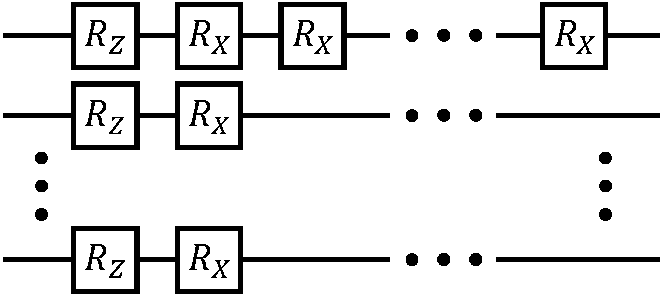
\includegraphics[width=0.9\textwidth]{figures/Z_Ansatz.pdf} \caption{难以多项式时间模拟的线路例子:每个量子比特上有一层 $R_Z$ 门,每个量子比特上有一层 $R_X$ 门,第一个量子比特上有 $L-2$ 层 $R_X$ 门。}\label{ap:prop:fig:ansatz} 
\end{figure}

如果截断含噪声期望值 $\abs{\bm{s}}\leq L$,估计的期望值可以表示为: 
\begin{equation} 
    \widehat{\langle O \rangle}=\sum_{\abs{s}\leq L} f(\widetilde{\mathcal{U}},\bm{s},O,\rho)=\sum_{m=0}^L (1-\lambda)^m \sum_{\abs{s}=m} f(\mathcal{U},\bm{s},O,\rho).
\end{equation}

在考虑 $\widetilde{\langle O \rangle}$ 和 $\widehat{\langle O \rangle}$ 之间的差异之前,我们首先考虑无噪声情况。第一个量子比特上的酉矩阵可以表示为: 
\begin{equation} 
    U|_1=\exp{-i\frac{\theta_{2,1}+\cdots+\theta_{L,1} }{2}X_1}\exp{-i\frac{\theta_{1,1}}{2}Z_1}.
\end{equation} 
记 $\alpha=\frac{\theta_{2,1}+\cdots+\theta_{L,1} }{2}$,无噪声理想期望值可以表示为: 
\begin{equation}\label{ap:eq:noiseless_cost} 
    \begin{aligned} 
        \langle O \rangle&=\bra{0}\exp{-i\frac{\theta_{1,1}}{2}Z_1}^\dagger\exp{-i \alpha X_1}^\dagger (Z_1+Y_1) \exp{-i \alpha X_1}\exp{-i\frac{\theta_{1,1}}{2}Z_1}\ket{0}\\
        &=\cos{2\alpha}-\sin{2\alpha}. 
    \end{aligned} 
\end{equation}

注意在第~\ref{sec:obppp}节中,我们讨论了对于具有非零贡献的 Pauli 路径 $\bm{s}$,必须有 $\abs{s_i} > 0$ 对于 $i=0,\cdots,L$成立。因此需要 $\abs{\bm{s}}\geq L+1$。

相反,若对于某个Pauli路径$\bm{s}$,如果 $\abs{\bm{s}}> L+1$且存在一个量子比特 $k\neq 1$,使得 $s_{i}|_k$ 在某些层 $i$ 上不是单位算符,则因为$O|_k=I$,会有 $f(\mathcal{U},\bm{s},O,\rho)=0$ 成立。
因此,对 $\langle O \rangle(\theta)$ 有非零贡献的 Pauli 路径 $\bm{s}$ 必须满足 $\abs{s}=L+1$。 
我们可以得出结论: 
\begin{equation}\label{ap:eq:noiseless_cost_2} 
    \begin{aligned} \langle O \rangle=\sum_{s\in \bm{P}^{L+1}_n} f(\mathcal{U},\bm{s},O,\rho)=\sum_{\abs{\bm{s}}=L+1} f(\mathcal{U},\bm{s},O,\rho).
    \end{aligned} 
\end{equation}

结合等式~\eqref{ap:eq:noiseless_cost} 和式~\eqref{ap:eq:noiseless_cost_2},可以得到: 
\begin{equation} 
    \mathbb{E}_{\bm{\theta}}\langle O \rangle^2=\mathbb{E}_{\bm{\theta}} \left[\sum_{\abs{s}=L+1} f(\mathcal{U},\bm{s},O,\rho) \right]^2=\mathbb{E}_{\alpha}(\cos{2\alpha}-\sin{2\alpha})^2=\mathbb{E}{\alpha}[1-\sin4\alpha]=1. 
\end{equation} 
上述方程中的最后一个等式是因为 $\alpha$ 遵循广义 Irwin-Hall 分布,其特征函数 $\varphi_{\alpha}(t)=\mathbb{E}[e^{it\alpha}]$ 可以表示为 $\left(\frac{e^{i\frac{\pi}{2}t}-e^{-i\frac{\pi}{2}t}}{i\pi t}\right)^{L-1}$。于是,有 
\begin{equation} 
    \mathbb{E}_{\alpha}[\sin4\alpha]=\textrm{Im }\mathbb{E}[e^{i4\alpha}]=\textrm{Im }\varphi_{\alpha}(4)=\textrm{Im }\left(\frac{e^{2\pi i}-e^{-2\pi i}}{4\pi i}\right)^{L-1}=0.
\end{equation}

综上所述,对于$\widetilde{\langle O \rangle}$ 和 $\widehat{\langle O \rangle}$ 之间的均方误差可以估计为: 
\begin{equation} 
    \begin{aligned} 
        \mathbb{E}_{\bm{\theta}}\abs{\widetilde{\langle O \rangle}-\widehat{\langle O \rangle}}^2 &=\mathbb{E}_{\bm{\theta}}\left[\sum_{\abs{s}> L}f(\widetilde{\mathcal{U}},\bm{s},O,\rho)\right]^2\\
         &=\mathbb{E}_{\bm{\theta}}\left[\sum_{\abs{s}=L+1}f(\widetilde{\mathcal{U}},\bm{s},O,\rho)\right]^2\\
        &= (1-\lambda)^{2(L+1)}\mathbb{E}_{\bm{\theta}} \left[\sum_{\abs{s}=L+1}{f}(\mathcal{U},\bm{s},O,\rho)\right]^2\\ 
        &=(1-\lambda)^{2(L+1)}.
    \end{aligned} 
\end{equation}

根据伯努利不等式,对于 $r\geq 1$ 和 $x\geq -1$,有 
\begin{equation} 
    (1+x)^r\geq 1+r. 
\end{equation}

由于 $\lambda=\order{\frac{1}{L}}$,存在一个常数 $c$ 使得 $c\geq \lambda (L+1)$。因此,我们有 \begin{equation} 
    (1-\lambda)^{2(L+1)}= (1-\lambda)^{\frac{2(L+1)}{4c} 4c} \geq \left(1-\lambda \frac{2(L+1)}{4c} \right)^{4c}\geq \left(\frac{1}{2}\right)^{4c}, 
\end{equation} 
此时有
\begin{equation} 
    \mathbb{E}_{\bm{\theta}}\abs{\widetilde{\langle O \rangle}-\widehat{\langle O \rangle}}^2 =\Omega(1). 
\end{equation}

所以截断 $\abs{s}\leq L$ 是不够的。 而具有非零贡献且满足 $\abs{\bm{s}}=L+1$ 的 Pauli 路径的数量为 $2^{L-1}$,具体为:
\begin{equation} 
    \begin{aligned}
        &\bm{s}=(s_0,s_1,\cdots,s_L)=(Z_1,Z_1,\cdots,Z_1,Y_1),\\
        &s_0=Z_1, \quad s_1=Z_1, \quad s_2=\begin{cases}
            Z_1 \\ \text{或}\\
            Y_1,
        \end{cases}
        \cdots, s_L=\begin{cases}
            Z_1 \\ \text{或} \\
            Y_1,
        \end{cases}
    \end{aligned}
\end{equation}
其中,$Z_1$ 和 $Y_1$ 分别表示第一个量子比特上的 Pauli 算符 $Z$ 和 $Y$。

因此,对于 $\gamma=\order{\frac{1}{L}}$,我们需要考虑所有具有非零贡献的 Pauli 路径,这将导致指数时间成本。这完成了命题~\ref{prop:lambda_and_L}的证明。


\section{本章小结}

本章介绍了变分量子线路的基本结构,以及对含噪声环境下模拟变分量子的意义。并使用基于Pauli路径积分的OBPPP算法实现对含噪声变分量子线路的模拟,并分析了算法的复杂度及对应的模拟误差。最后,我们讨论了在噪声率与线路深度之间的关系下,模拟算法的有效性。

主要结果通过定理~\ref{thm:main}刻画,即对于含有常数噪声的变分量子线路,在满足初始态密度矩阵和观测量都是稀疏以及条件~\ref{eq:generate}成立的情况下,存在多项式量级的经典算法可以在高效近似地模拟含噪声的变分量子线路。这意味着在考虑现有实验条件下,在NISQ设备上运行的变分量子算法很难相对经典算法提供实际的量子优势。

此外,我们还探讨了在未来量子设备的发展中,若要在含噪声的设备上实现量子优势需要满足的必要条件,该结果通过命题~\ref{prop:lambda_and_L}呈现。需要设备的噪声率$\gamma$与线路深度$L$满足$\gamma=o(\frac{1}{\log L})$,才有可能呈现出量子优势。这一结果对于未来量子设备的发展具有一定的指导意义。
\chapter{数值模拟}

在过去的章节中,我们介绍了量子线路的基本概念,并介绍了如何使用基于Pauli路径积分的模拟算法来模拟量子线路。并在一些具体的线路模型中,研究了模拟算法的计算复杂度和误差。特别地,发现了在一些情况下,比如含噪声的变分量子线路和Clifford扰动电路,算法的计算复杂度关于线路规模是多项式关系。
虽然,我们定性地分析了模拟算法的计算复杂度,但是我们还没有给出具体的数值模拟结果。多项式复杂度对于实际的模拟算法来说是一个很好的性质,但是是否实用还有待进一步的数值模拟结果的验证。
例如,在定理~\ref{thm:main}中,我们得到了对于噪声\textbf{情况1}时,算法的计算复杂度是:
\begin{equation*}
    \mathrm{Poly}(n) \order{L} \bigg(\frac{\norm{O}_\infty}{\varepsilon \sqrt{\delta}} \bigg)^{\order{\frac{1}{\gamma}}},
\end{equation*}
其中$n$是线路的规模,$L$是线路的深度,$\varepsilon$是算法的精度,$\delta$是算法失败的概率,$\gamma=\min\{p|{p \in \{p_x,p_y,p_z\},p\neq 0}\}$是噪声率,$\norm{O}_\infty$是可观测量的无穷范数。当噪声强度$\gamma$很小时,例如$\gamma=0.01$,我们可以得到算法的计算复杂度是$\mathrm{Poly}(n) \order{L} \bigg(\frac{\norm{O}_\infty}{\varepsilon \sqrt{\delta}} \bigg)^{{100}}$,这是一个难以实现的计算复杂度。万幸的是,实际情况下的计算复杂度并不会达到这么高的程度,我们将在本章中具体说明。

除此之外,在这一章中,我们将使用基于Pauli路径积分的模拟算法来模拟一些量子线路的具体实例。并与实际的实验结果进行比较,以验证模拟算法的有效性。




\section{含噪变分线路模拟的计算复杂度}
对于含噪声变分量子线路,可以使用OBPPP算法对其实现高效模拟,根据式~\eqref{eq:vqa:cost},在噪声\textbf{情况1}下,OBPPP模拟算法的计算复杂度是:
\begin{equation*}
    \mathrm{Poly}(n) \order{L}2^M,
\end{equation*}
其中$n$是线路的规模,$L$是线路的深度,$M$是截断变量。可以看到在过去理论估计中,计算复杂度关于截断变量$M$是指数关系。这个指数因子的来源是由于在Pauli 路径枚举过程中,根据式~\eqref{eq:vqa:case1:N_M},符合条件$\abs{\bm{s}}\leq M$的Pauli路径数目是指数级别的。在这一节中,我们将通过具体的数值模拟结果来估计,给定截断变量$M$时,满足条件Pauli路径的真实数目。



在本节中,我们将假设环境噪声处于\textbf{情况1},这是因为在实际的量子计算机中,很难出现纯净的单独类型的Pauli错误。因此假设$p_x\neq 0,p_y\neq 0,p_z\neq 0$是合理的,此时与噪声关联的Hamming Weight 根据式~\eqref{eq:noise_hamming_weight}可以得到:
\begin{equation*}
    \abs{\bm{s}}_{\mathcal{N}}=\abs{\bm{s}}_X + \abs{\bm{s}}_Y + \abs{\bm{s}}_Z.
\end{equation*}
在这种情况下,正是原始的Hamming Weight定义,为了方便,我们将在本章中使用$\abs{\bm{s}}$来表示。
为了方便,我们考虑的噪声模型,如未加说明,均为退极化噪声模型,即满足$p_x=p_y=p_z=\frac{\lambda}{4}$,其中$\lambda$是噪声强度。



%\subsection{计算复杂度与截断变量$M$的关系}

因为截断Pauli路径模拟算法的计算复杂度主要来自于具有非平凡贡献的Pauli路径的数量,因此我们将通过计算具有非零贡献的Pauli路径的数量来估计模拟算法的计算复杂度。在这一节中,我们将通过具体的数值模拟结果来估计,给定截断变量$M$时,满足条件Pauli路径的真实数目。


\begin{figure}[htbp]
    \centering
    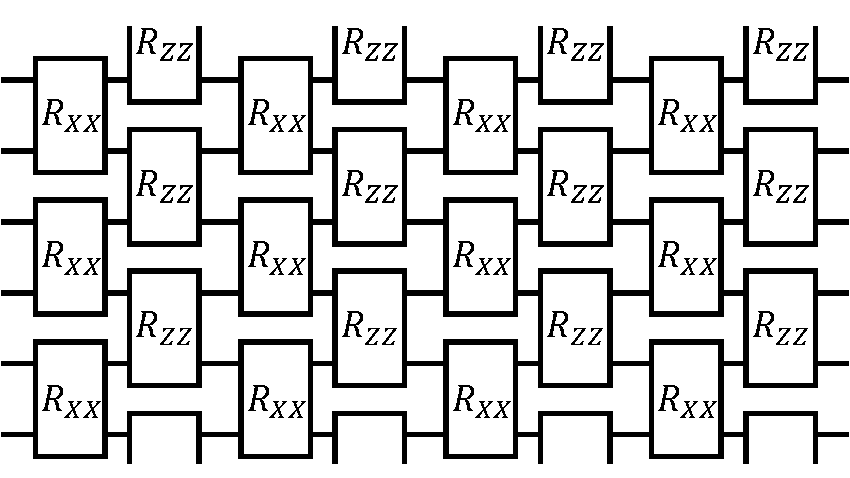
\includegraphics[width=0.5\textwidth]{figures/XX_ZZ_Ansatz.pdf}
    \caption{数值模拟计算复杂度与$M$的关系中使用的量子线路示意图}\label{fig:XX_ZZ_Ansatz}
\end{figure}

在我们的模拟中,我们考虑了一个具体的MaxCut问题实例。
对于给定的量子比特数$n$,我们随机生成一个$n\times n$的邻接$(0,1)$矩阵$A$,其中每个元素为$1$的概率为$0.5$。
可观测量$O$基于MaxCut问题构建,并按照给出的邻接矩阵$A$构造:
\begin{equation}
    O=\sum_{A_{i,j}=1} Z_iZ_j.
\end{equation}
在模拟中,初始状态的密度矩阵设为$\rho=\ketbra{0}{0}^{\otimes n}$。
考虑的量子线路$\mathcal{U}$如图~\ref{fig:XX_ZZ_Ansatz}所示,该线路由交替的$R_{XX}$和$R_{ZZ}$ 旋转门组成,其中第一个量子比特上的不完整$R_{ZZ}$门表示它们作用于第一个和最后一个量子比特。


\begin{figure}[hbp]
    \centering
    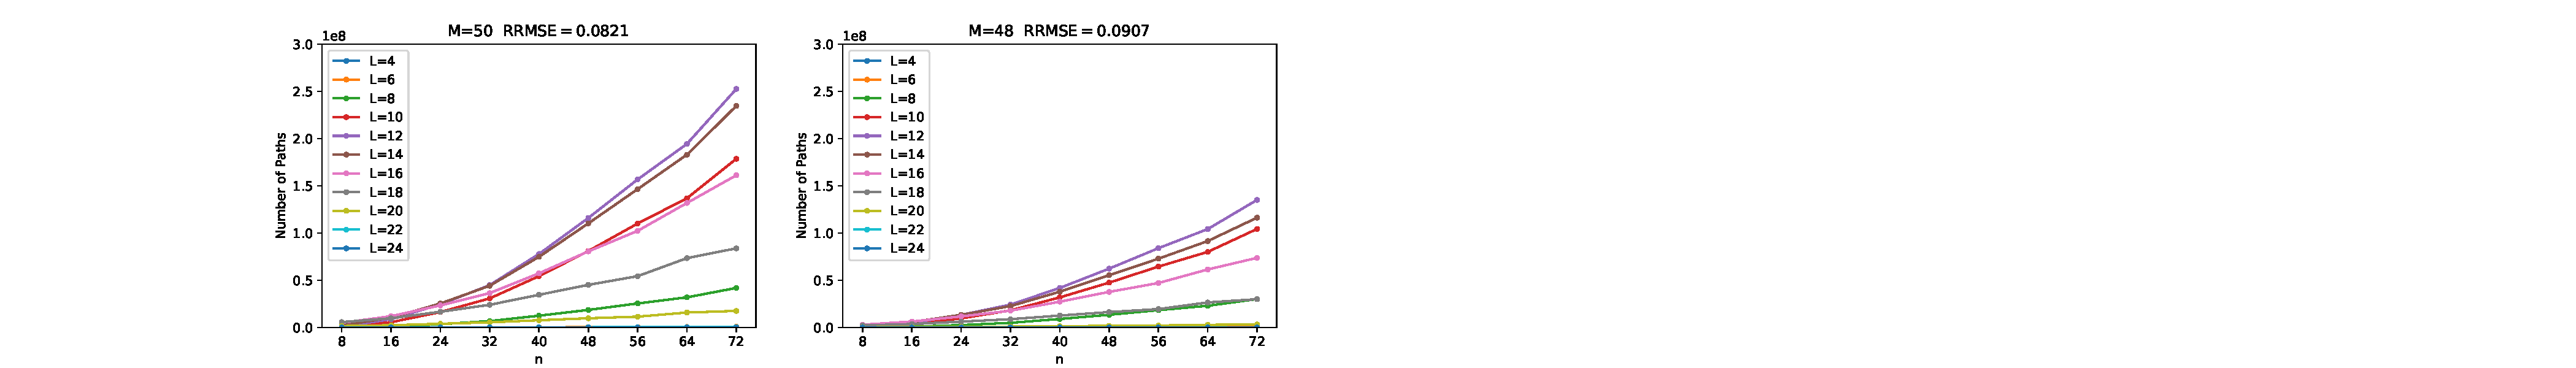
\includegraphics[width=\textwidth]{figures/depth_path2_p1}
    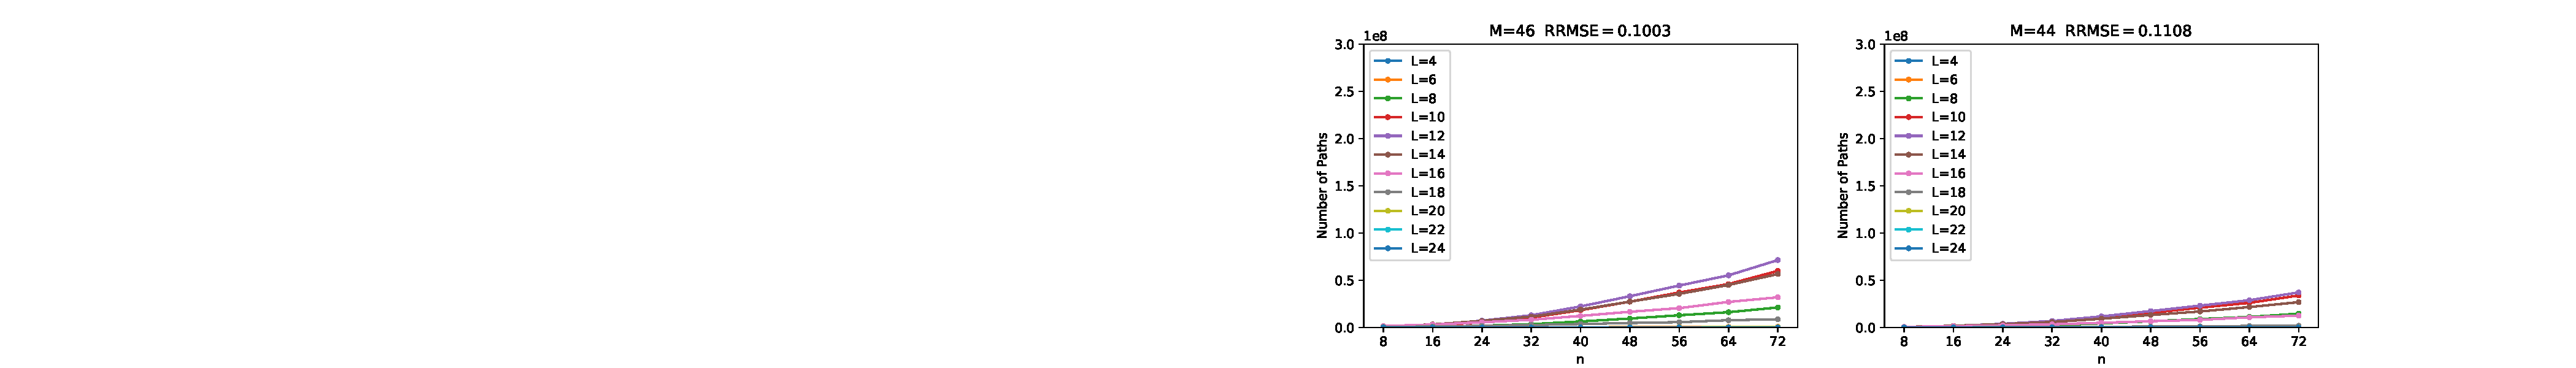
\includegraphics[width=\textwidth]{figures/depth_path2_p2}
    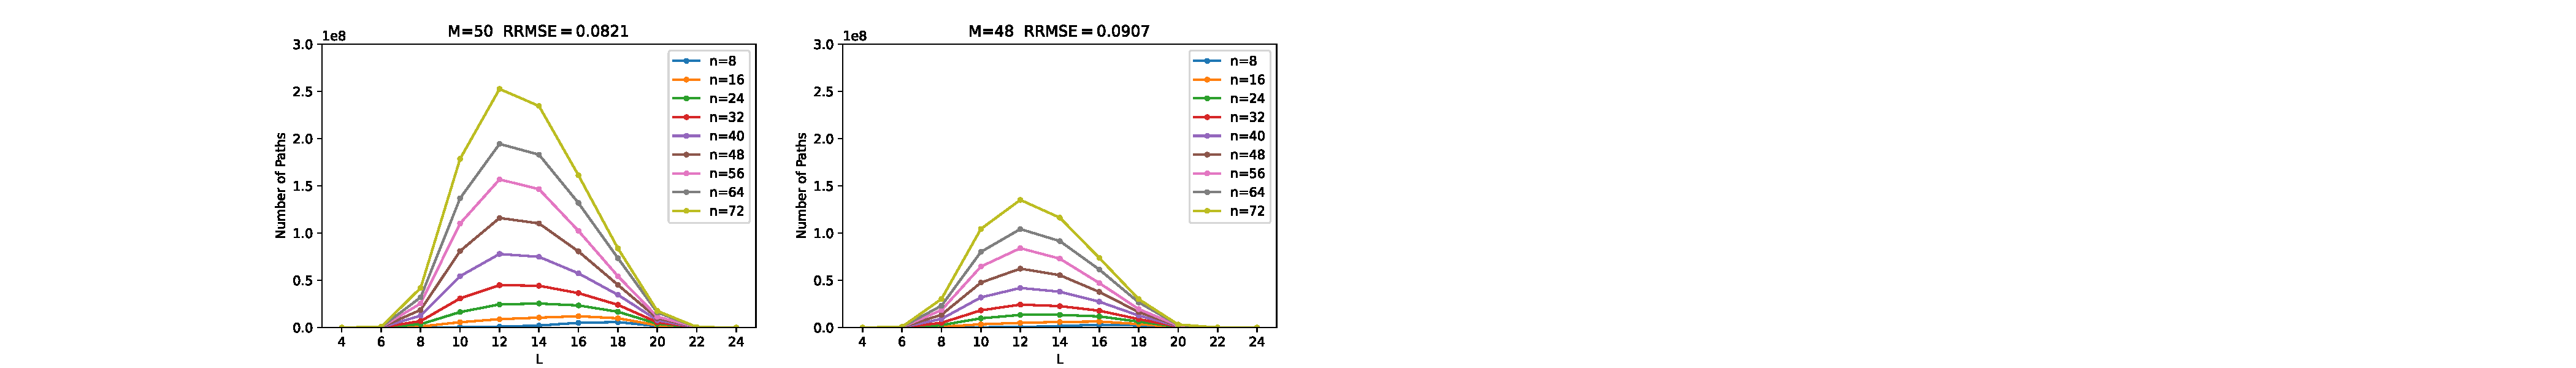
\includegraphics[width=\textwidth]{figures/depth_path_p1}
    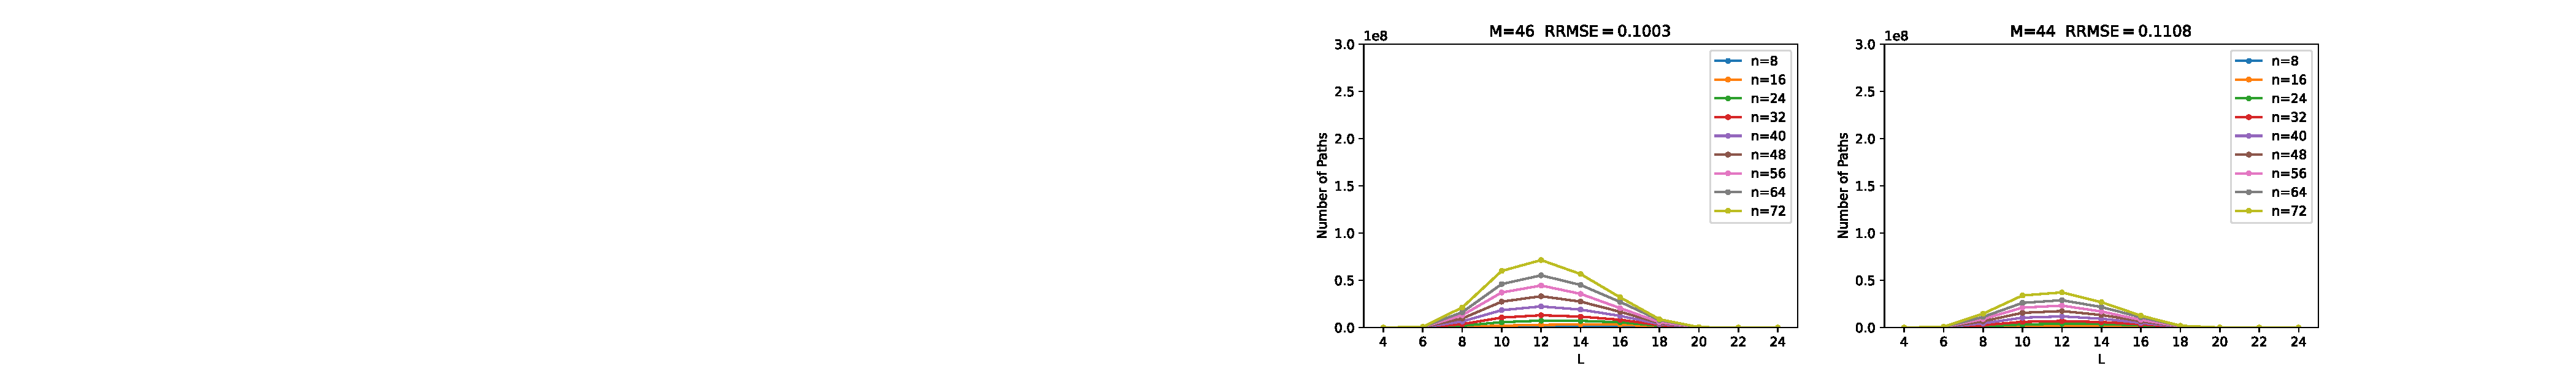
\includegraphics[width=\textwidth]{figures/depth_path_p2}
    \caption{具有非零贡献且$\abs{\bm{s}}\leq M$的Pauli路径$\bm{s}$的数量}\label{fig:numerical_cost}
\end{figure}

根据式~\eqref{eq:depolarizing_M:1},对于固定的量子线路,不同的截断参数$M$对应于在固定噪声率下由$\frac{\sqrt{\mathbb{E}_{\bm{\theta}}\abs{\widetilde{\langle O \rangle}-\widehat{\langle O \rangle}}^2}}{\norm{O}_\infty}$给出的相对均方根误差界(Relative Root Mean Square Error,RRMSE)。

对于不同的量子比特数$n$和线路的深度$L$,我们计算了权重$\abs{s}\leq M$且具有非零贡献的Pauli路径$s$的数量,结果如图~\ref{fig:numerical_cost}所示。前两行的每个图显示了在固定$M$的情况下,随着$n$的增加,具有非零贡献的Pauli路径的数量的变化。可以看到,在固定$M$的情况下,随着$n$的增加,对所有不同深度$L$的情况,具有非零贡献的Pauli路径的数量将适度增加,并显著小于理论分析的上界$\mathrm{Poly}(n)2^M$。


后两行的每个图显示了在固定$M$的情况下,随着$L$的增加,具有非零贡献的Pauli路径的数量的变化。我们观察到,对于给定的RRMSE界,路径数量先增加然后随着$L$的增加而减少。
这意味着,在给定精度下模拟含噪声量子线路的计算复杂度随着线路深度的增加呈现出先增加后减少的趋势。这与文献~\cite{noh2020efficient}中的发现一致。
其中的RRMSE界是由式~\eqref{eq:depolarizing_M:1}在噪声率$\lambda=0.2$下给出的。


另一方面,通过式~\eqref{eq:depolarizing_M:1},可以看到不同的截断参数$M$在给定的RRMSE界下也对应了一个具体的噪声强度$\lambda$。
假设,RRMSE界固定为$0.0821$,按图中给出的数据将$M$取值为$M=50,48,46,44$,此时对应的噪声强度为$\lambda=0.2,0.21,0.22,0.23$(两位有效数字)。
从数值结果中可以看到,对于不同的$M$,在给定线路规模$n$和深度$L$的情况下,具有非零贡献的Pauli路径的数量是不同的。这说明在实际的模拟中,噪声的大小将会显著影响模拟算法的计算复杂度。


\section{含噪变分量子线路模拟的误差}

在本节中,我们研究了OBPPP算法在实现可靠精度的情况下,在不同电路规模下截断数$M$的要求。

对于截断变量$M$的取值,根据引理~\ref{lemma:MSE_l}的注释,我们可以得到
对于变分量子线路在退极化噪声下,如果式~\eqref{eq:E_cross_equals_0}成立,那么对任意的$\nu > 0$,只要截断参数$M$满足:
\begin{equation}\label{eq:depolarizing_M}
    M\geq\frac{1}{2\lambda}\ln{\frac{\norm{O}_\infty^2}{\nu}},
\end{equation}
其中$\lambda$是退极化噪声的强度,那么含噪声期望值模拟的均方误差满足:
\begin{equation}
    \mathbb{E}_{\bm{\theta}}\left[\left(\widetilde{\langle O\rangle}-\widehat{\langle O\rangle}\right)^2\right]\leq\nu.
\end{equation}
事实上,在实际计算中,$M$并不需要取到这么大的值,我们将在本节中具体用数值说明。


与前一节类似,我们也以MaxCut问题对应的可观测量为例,在数值上分析$M$与线路规模之间的关系。
对于给定的量子比特数$n$,我们随机生成一个$n\times n$的邻接$(0,1)$矩阵$A$,其中每个条目为$1$的概率为$0.5$。
可观测量为$O=\sum_{A_{i,j}=1} Z_iZ_j$。
初始状态的密度矩阵设为$\rho=\ketbra{0}{0}^{\otimes n}$。

在这一节的模拟中,考虑的量子线路是硬件高效变分量子线路(Hardware Efficient Ans\"atz)~\cite{kandala2017hardwarea}的一个例子,如图~\ref{fig:HEA_Ansatz}所示。
该线路由一系列单量子比特旋转和纠缠的双量子比特门组成,可以分割为$D$个深度为$4$的线路块,每个模块包含两层层作用在所有量子比特上的单量子比特$R_X$和$R_Z$旋转门,以及两层分别以奇数量子比特为控制位和偶数量子比特为目标位的CNOT门。
值得注意的是,双量子比特门的应用仅限于相邻的量子比特,这一设计适合于当前阶段NISQ设备的硬件限制。
对于给定的重复次数$D$,该硬件高效变分量子线路的深度为$4\times D+2$,参数的数量为$2\times D+2$。



\begin{figure}[htbp]
    \centering
    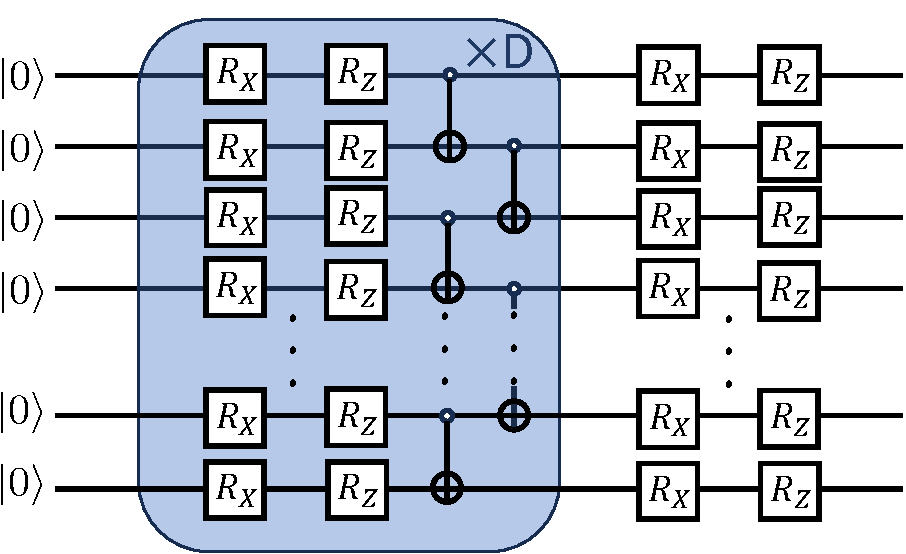
\includegraphics[width=0.5\textwidth]{figures/complexity2/HEA.pdf}
    \caption{Hardware Efficient Ans\"atz}\label{fig:HEA_Ansatz}
\end{figure}

我们随机均匀生成$100$个参数组,记为$\bm{\theta^1}\cdots \bm{\theta^{100}}$,其中每个参数$\bm{\theta^i}$是一个长度为$2\times D+2$的向量,每个元素在$[0,2\pi]$之间均匀分布。
为了方便,记参数取值为参数组$\bm{\theta}$时的含噪声期望值为$\widetilde{\langle O \rangle}(\bm{\theta})$,使用截断数为$M$的Pauli路径积分方法估计的含噪声期望值为$\widehat{\langle O \rangle}(\bm{\theta})$。
我们的数值模拟目标是,找到满足近似含噪声期望值$\widehat{\langle O \rangle}(\bm{\theta})$与精确含噪声期望值$\widetilde{\langle O \rangle}(\bm{\theta})$之间的相对差异在$100$个参数组上均低于$0.1\%$的最小截断数$M$:
\begin{equation}
    \begin{aligned}
        \text{minimize} \quad & M,\\
        \text{subject to} \quad & \widehat{\langle O \rangle}=\sum_{\abs{\bm{s}}\leq M}f(\widetilde{\mathcal{U}},\bm{s},O,\rho),\\
        &\max_{i}\frac{\abs{\widetilde{\langle O \rangle}(\bm{\theta^i})-\widehat{\langle O \rangle}(\bm{\theta^i})}}{\abs{\widetilde{\langle O \rangle}(\bm{\theta^i})}}\leq 0.001.
    \end{aligned}
\end{equation}

\begin{figure}[htbp]
    \centering
    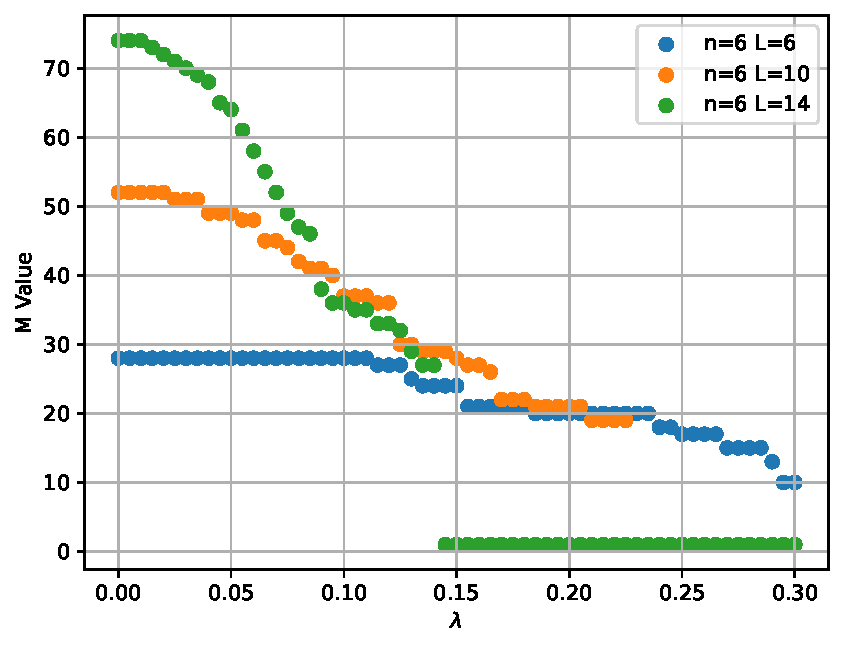
\includegraphics[width=0.45\textwidth]{figures/complexity2/6}
    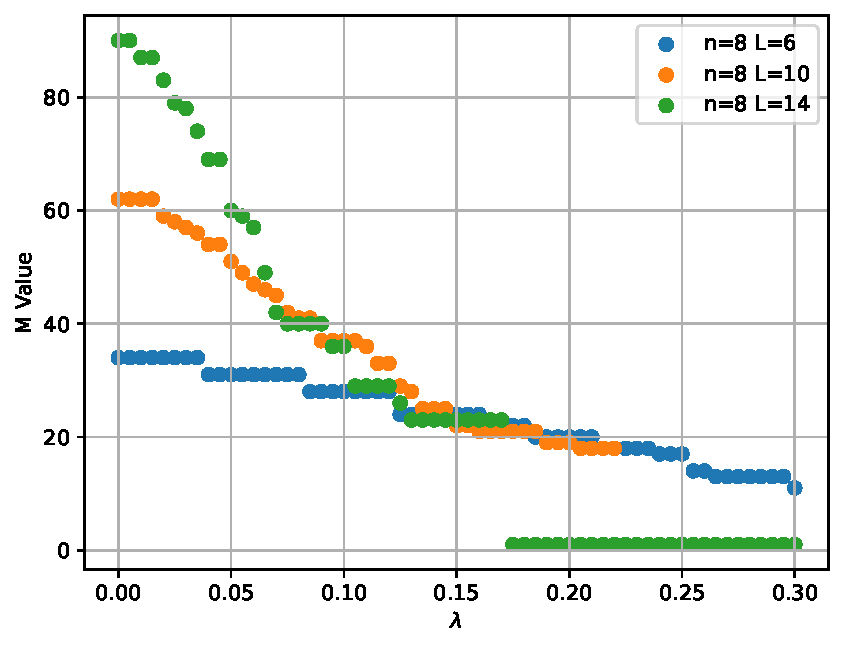
\includegraphics[width=0.45\textwidth]{figures/complexity2/8}
    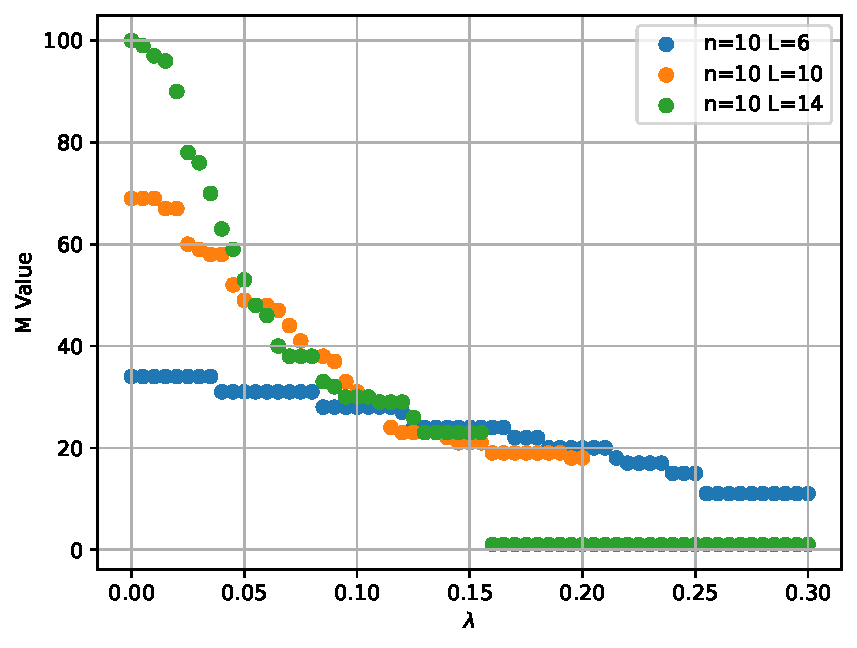
\includegraphics[width=0.45\textwidth]{figures/complexity2/10}
    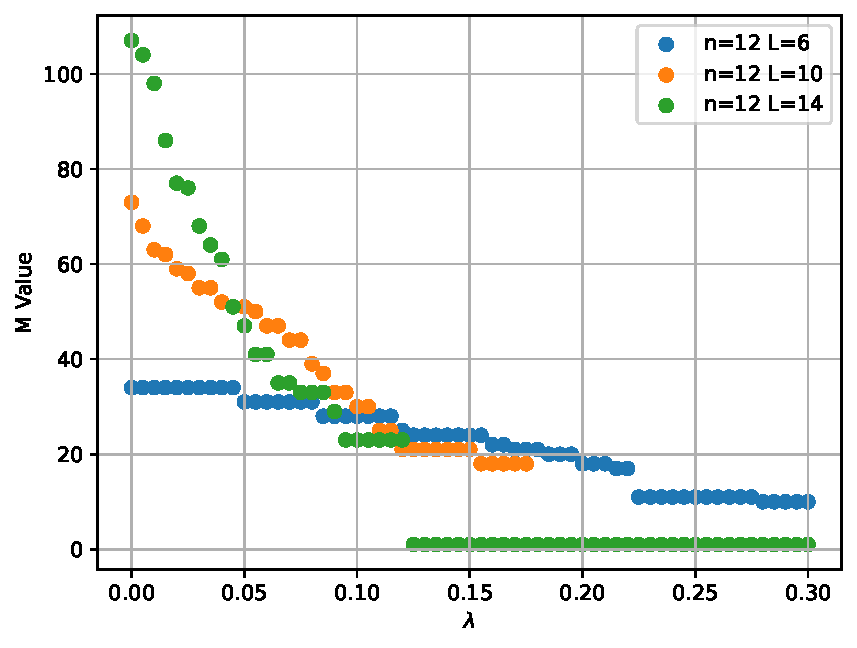
\includegraphics[width=0.45\textwidth]{figures/complexity2/12}
    \caption{满足相对误差要求的最小截断$M$的取值}\label{fig:numerical_M}
\end{figure}

结果如图~\ref{fig:numerical_M}所示。
首先,我们观察到在所有情况下,最小截断$M$随着噪声率$\lambda$的增加而减少。这一趋势与引理~\ref{lemma:MSE_l}中的理论分析一致。
数值结果表明,当噪声率保持在较低水平时,最小截断值$M$随着电路深度$L$线性增加。
这一趋势是由于噪声对Pauli路径的影响较小,导致在浅电路中Pauli路径的传播距离随着电路变深而增加,从而提高了它们的Hamming Weight。因此,在量子线路变深的过程中,为了保留相关的Pauli路径不被丢弃,截断变量$M$需要增加。

当噪声强度较大时,电路深度$L$对于最小截断值$M$的减少速率方面起着关键作用。
这一现象是由于噪声的累积随着电路深度的增加而加剧,导致期望值$\widetilde{\langle O \rangle}(\bm{\theta})$更快地收敛到$\tr{O}$(平凡Pauli路径的贡献)。因此,对于电路深度更深的情况,最小截断值$M$更快地收敛到$0$。

此外,随着量子比特数$n$的增加,最小截断值$M$也趋于增加。
然而,这一增加是适度的,表明OBPPP方法在实际应用中,并不会过度受限于量子比特数$n$的规模。

我们还探讨了在给定电路规模时,精度与截断数$M$之间的关系。当$n = 12$时,我们确定了实现不同精度水平所需的最小$M$值:
\begin{equation}
    \begin{aligned}
        \text{minimize} \quad & M,\\
        \text{subject to} \quad & \widehat{\langle O \rangle}=\sum_{\abs{\bm{s}}\leq M}f(\widetilde{\mathcal{U}},\bm{s},O,\rho),\\
        &\max_{i}\frac{\abs{\widetilde{\langle O \rangle}(\bm{\theta^i})-\widehat{\langle O \rangle}(\bm{\theta^i})}}{\abs{\widetilde{\langle O \rangle}(\bm{\theta^i})}}\leq 0.1,0.05,0.01,0.001,0.0001,0.00001,
    \end{aligned}
\end{equation}
分别对应于$90\%,95\%,99\%,99.9\%,99.99\%,99.999\%$的精度。
结果如图~\ref{fig:numerical_ACC}所示,表明所需的最小截断值$M$随着所需精度的增加而增加。


\begin{figure}[htbp]
    \centering
    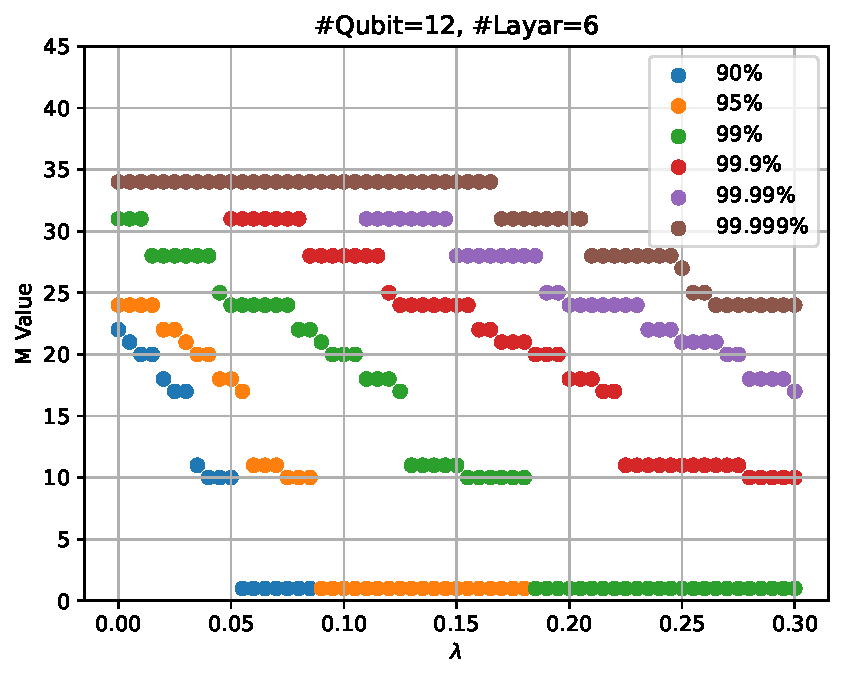
\includegraphics[width=0.32\textwidth]{figures/complexity2/ACC1}
    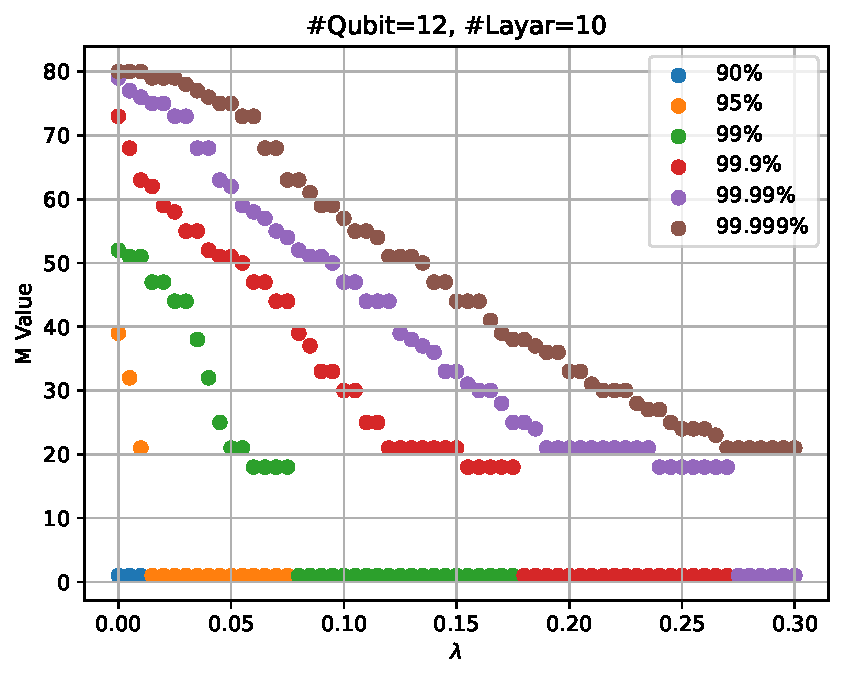
\includegraphics[width=0.32\textwidth]{figures/complexity2/ACC2}
    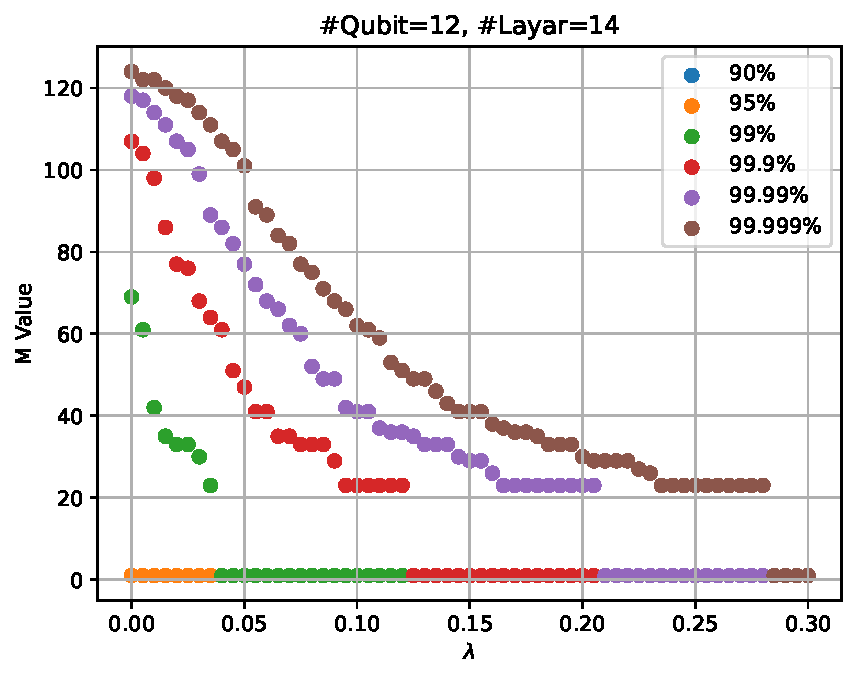
\includegraphics[width=0.32\textwidth]{figures/complexity2/ACC3}
    \caption{
        不同精度水平下所需的最小截断值$M$}\label{fig:numerical_ACC}
\end{figure}

从数值结果可以看出,当对精度的需求迅速增加时,对$M$的需求增加相对温和。
在$L=6$且噪声率$\lambda<0.05$的情况下,实现$>99.9\%$精度所需的最小$M$约为$34$。注意,图中显示的$99.9\%$和$99.99\%$精度对应的结果被$99.999\%$的结果所掩盖。
当噪声率$\lambda$接近$0$时,实现高精度($\geq 99.9\%$)所需的$M$值趋于相同,表明此时$M$足够大以涵盖计算中的足够多的Pauli路径。

当噪声率$\lambda$增加时,实现低精度所需的$M$将比实现高精度所需的$M$减少得更快,这一趋势与引理~\ref{lemma:MSE_l}一致。

对于实现$99.9\%$精度所需的最小截断值$M$,我们通过以下公式估计取定该$M$值时经验均方误差$\tilde{\nu}$:
\begin{equation}\label{ap:eq:emse}
    \tilde{\nu} = \frac{1}{100}\sum_{i=1}^{100}\left|\widetilde{\langle O \rangle}(\bm{\theta^i}) - \widehat{\langle O \rangle}(\bm{\theta^i})\right|^2,
\end{equation}
其中
\begin{equation}
    \begin{aligned}
        \widehat{\langle O \rangle}=&\sum_{\abs{\bm{s}}\leq M}f(\widetilde{\mathcal{U}},\bm{s},O,\rho),\\
        M=&\arg\min_{M} \left\{ \max_{i} \frac{\left|\widetilde{\langle O \rangle}(\bm{\theta^i}) - \widehat{\langle O \rangle}(\bm{\theta^i})\right|}{\left|\widetilde{\langle O \rangle}(\bm{\theta^i})\right|} \leq 0.001 \right\}.
    \end{aligned}
\end{equation}
然后将$M$与由式~\ref{eq:depolarizing_M}给出的关于$M$解析界进行比较:
\begin{equation}\label{ap:eq:analytical_bound}
  \frac{1}{2\lambda}\ln{\frac{\norm{O}_\infty^2}{\tilde{\nu}}}.
\end{equation}

\begin{figure}[htbp]
    \centering
    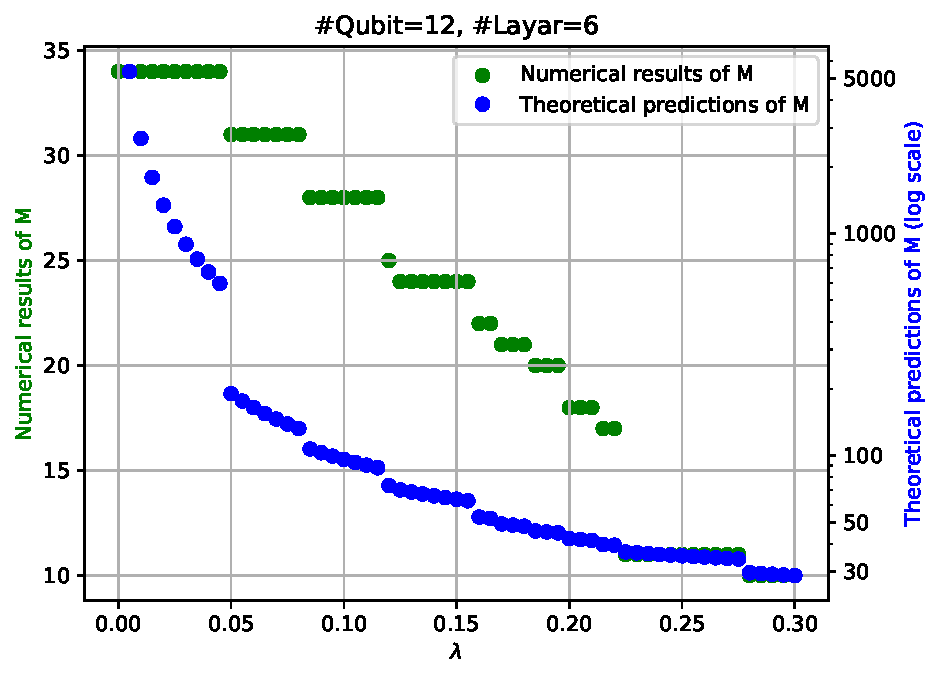
\includegraphics[width=0.32\textwidth]{figures/complexity2/12_1}
    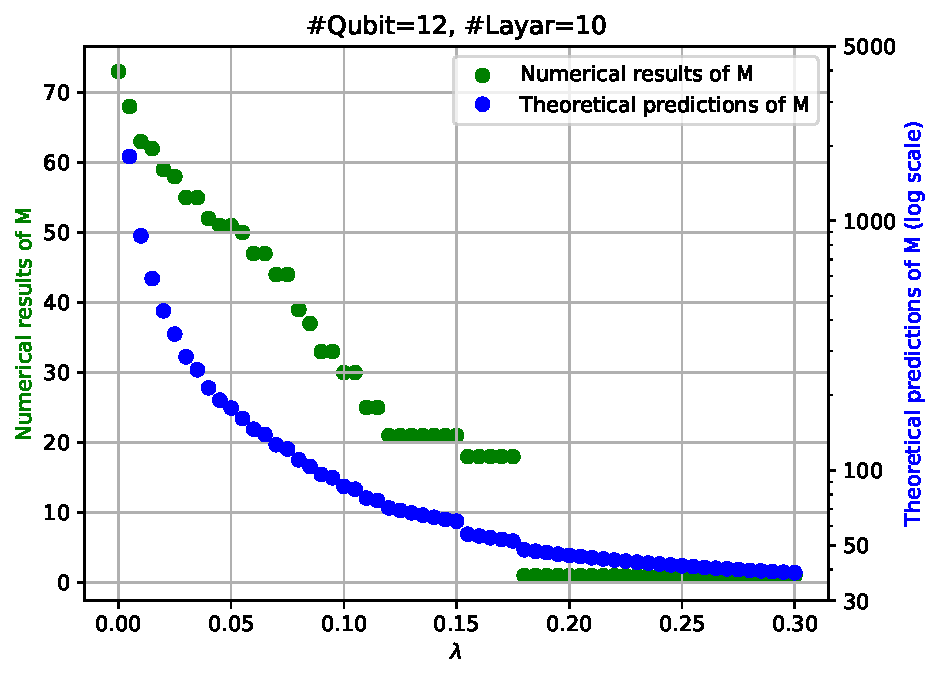
\includegraphics[width=0.32\textwidth]{figures/complexity2/12_2}
    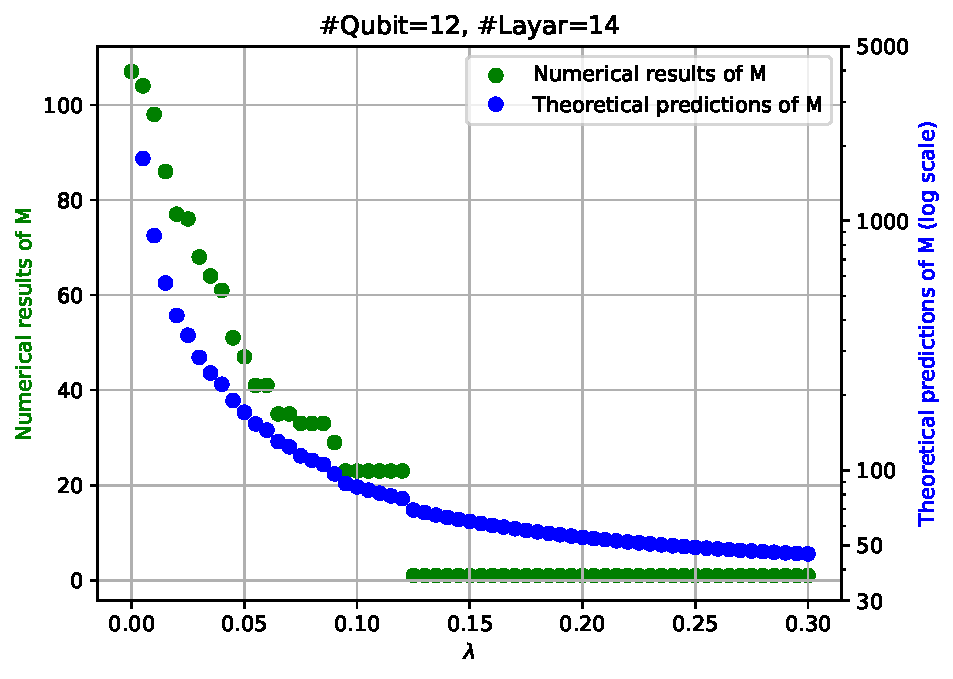
\includegraphics[width=0.32\textwidth]{figures/complexity2/12_3}
    \caption{
        实际应用中所需的最小截断数$M$与理论解析估计的比较}\label{fig:numerical_M2}
\end{figure}

量子比特数$n=12$的对应结果如图~\ref{fig:numerical_M2}所示(其他情况类似)。理论的解析估计结果记为\textit{``Theoretical predictions of M"},为了清晰起见,理论估计的数据使用对数轴显示在右侧。
为了避免式~\eqref{ap:eq:analytical_bound}的分母为$0$,移除了$\lambda=0$的解析估计结果。
结果表明,在实际情况下,为达到目标精度所需的$M$值显著低于理论估计的边界($\sim 100$ vs $\sim 5000$)。

最后,我们展示了在不同噪声率$\lambda$下,经验均方误差$\tilde{\nu}$随$M$增加的变化趋势,以显示收敛趋势。对于$n=12$的情况,如图~\ref{fig:numerical_MSE}所示。
y轴表示经验均方误差,由公式~\ref{ap:eq:emse}给出,并以对数刻度显示。
注意,在图\#Layer=6的数据中中,省略了$M=34$的结果,此时均方误差的值降到了$e^{-20}$以下。

\begin{figure}[htbp]
    \centering
    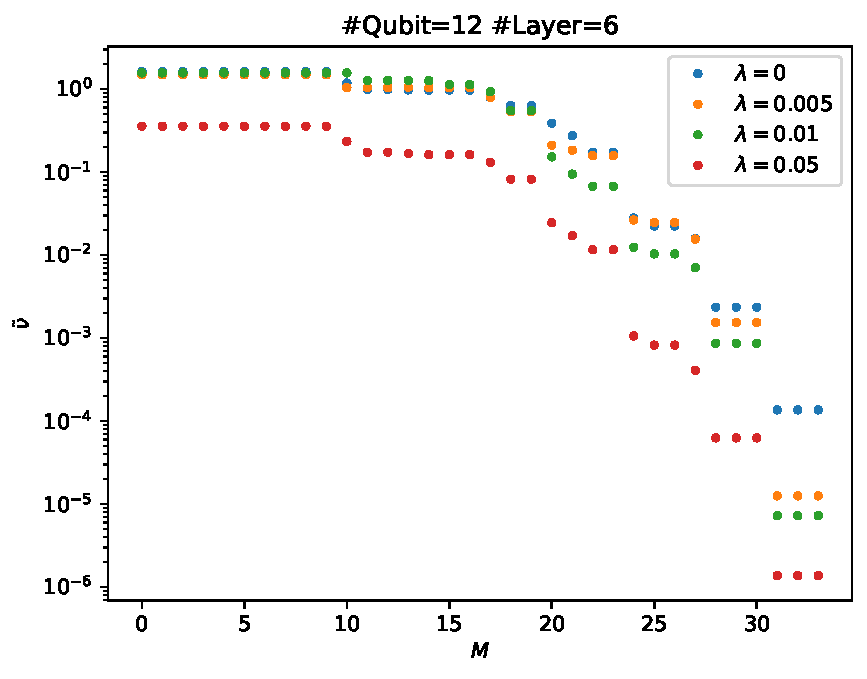
\includegraphics[width=0.32\textwidth]{figures/complexity2/mse_12_6.pdf}
    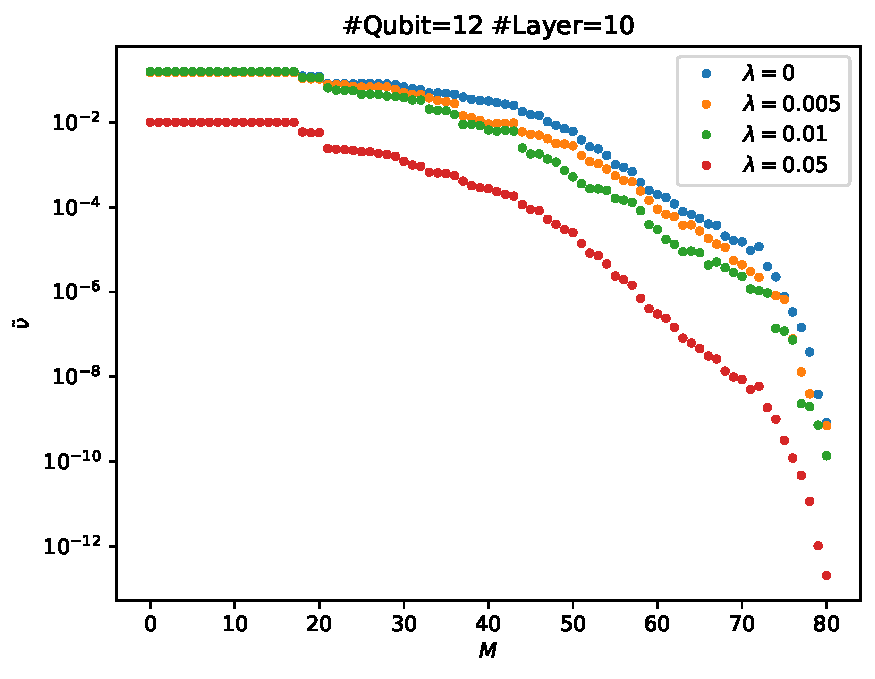
\includegraphics[width=0.32\textwidth]{figures/complexity2/mse_12_10.pdf}
    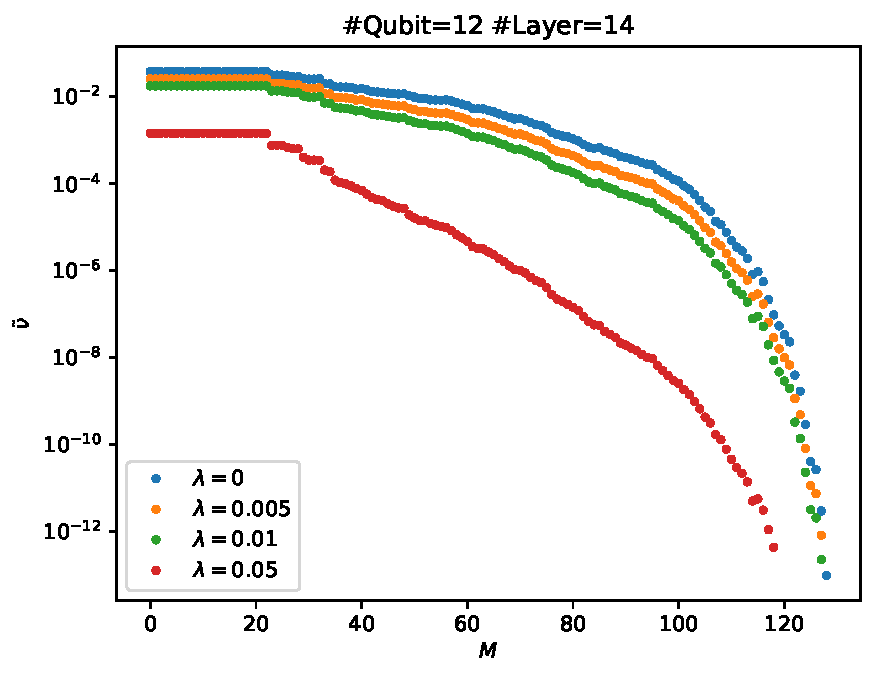
\includegraphics[width=0.32\textwidth]{figures/complexity2/mse_12_14.pdf}
    \caption{对于不同噪声率$\lambda$,$M$增加时的均方误差的变化趋势}\label{fig:numerical_MSE}
\end{figure}


\section{Clifford扰动线路模拟的误差}
对于Clifford扰动量子线路,可以使用SPD方法对其实现高效模拟,并能在小角度空间$\Theta=\{\bm{\theta}\mid \abs{\theta_i}\leq \theta_* ,i=1,\cdots,L \}$上实现高精度模拟。

根据定理~\ref{thm:spd},在理论结果中,我们证明了如果最大角度限制为$\theta_*=\frac{\ln{1+\frac{\delta}{2}}}{L-M}$,则在小角度空间$\bm{\theta}\in\Theta=\{\bm{\theta}\mid \abs{\theta_i}\leq \theta_* ,i=1,\cdots,L \}$内,截断误差可以被限制在$\abs{\langle O \rangle - \langle O \rangle ^{(M)}}\leq \delta$。从理论结果出发,为了达到$10^{-2}$的精度,解析结果表明$\theta_*$应约为$\ln{1+\frac{10^{-2}}{2}}\approx 0.005$,这是一个非常狭窄的区间。

过小的可用小角度空间将会为CPDR框架准备足够的训练数据时带来困难。
幸好在实际情况中,当截断数$M$适中(例如$M=5,7$)时,数值结果在更广泛的角度范围内仍然非常准确,使得这种方法得以适用于实际场景。


在本节中,我们在文献~\cite{sim2019expressibility}中提出的硬件高效电路上对SPD模拟器进行基准测试。
硬件高效电路由多个重复块组成,每个块的结构如图~\ref{fig:hardware_block}所示,其中首先包含一层$R_X$旋转门和一层$R_Z$旋转门,然后紧随其后的是按顺序作用在相邻量子比特上的CNOT门。
在我们的设置中,我们测试的量子电路包含五个块,量子比特数量从2到15不等。此外,每个门的旋转角度在整个电路中被设置为是相同的,且范围在$[0,\pi/4]$之间。

\begin{figure}[!ht]
    \centering
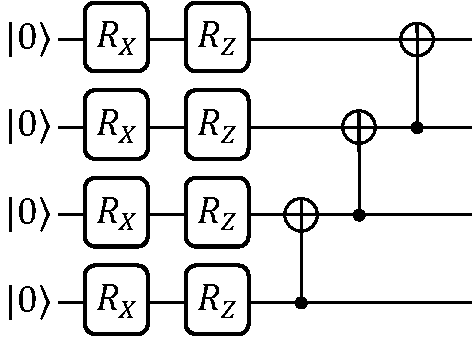
\includegraphics[width=0.5\textwidth]{figures/circuit_20241207.pdf}
    \caption{硬件高效电路中每个块的结构}
\label{fig:hardware_block}
\end{figure}


第一个模拟结果展示了,在固定量子比特数为$n=15$的电路中,误差$\abs{\langle O \rangle - \langle O \rangle^{(M)}}$随旋转角度$\theta_*$的变化。
如图~\ref{fig:bench_mini_AQC}(a)所示,当$\theta_*\leq \pi/20$时,截断误差随着截断数$M$的增加迅速减少。对于$10^{-2}$的精度,$\theta_*\leq \pi/20$对于$M\geq 5$是足够的。此外,当$M=11$时,截断误差在$\theta_*=\pi/8$之前保持在$10^{-2}$以内。这表明稍大一些的$M$值可以在实际场景中显著提高精度,超出理论界限。

为了评估大规模量子电路的可扩展性,我们评估了不同截断数$M$和量子比特数量在$[2,15]$范围内的截断误差$\abs{\langle O \rangle - \langle O \rangle ^{(M)}}$。考虑到SPD模拟器用于为CPDR框架提供训练数据,我们将每个旋转门的角度设置为适当的值以准备训练数据。基于数值测试的经验结果,我们建议将$\theta_* = \pi/20$并从$\Theta$中获取训练数据,以平衡训练集大小和模拟精度。如图~\ref{fig:bench_mini_AQC}(b)所示,展示了在给定旋转角度$\theta_*=\pi/20$时,误差随量子比特数$n$的变化。随着量子比特数量的增加,误差在$M\geq 5$时保持在$10^{-2}$以下,这表明SPD模拟器对于大规模量子电路是可扩展的。


\begin{figure}[!ht]
    \centering
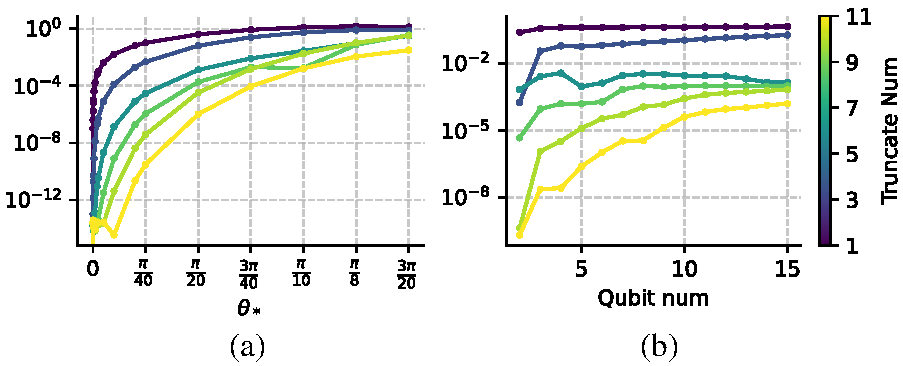
\includegraphics[width=\textwidth]{figures/SPD_benchmark.pdf}
    \caption{SPD模拟器在硬件高效电路上的基准测试}
\label{fig:bench_mini_AQC}
\end{figure}

\section{127-quibit Ising模型演化实验模拟}



在本节中,我们通过对IBM的127量子比特Eagle处理器~\cite{kim2023evidence}进行经典模拟来验证OBPPP方法在实际应用中的效率。
在文献~\cite{kim2023evidence}中,IBM报告了在127量子比特Eagle处理器上的实验,并展示了在一些特定可观测量下期望值的测量。所用的量子线路是由二维横场Ising模型的Trotter时间演化构建的,并被设计为符合Eagle处理器的拓扑结构。
整个量子系统的时间动力学由哈密顿量:
\begin{equation}
  H=-J\sum_{\langle i,j\rangle} Z_iZ_j+h\sum_i X_i,
\end{equation}
控制,其中$J$是耦合强度,$h$是横场强度,$\langle i,j\rangle$表示最近邻的量子比特对。
系统演化过程可以通过哈密顿量的一阶Trotter时间演化来模拟:
\begin{equation}
    \begin{aligned}
        U(\tau)&=\exp{-i\tau H}=\prod_{\langle i,j\rangle} \exp{i\tau J Z_iZ_j}\prod_i \exp{-i\tau h X_i}+\order{\tau^2}\\
        &=\prod_{\langle i,j\rangle}R_{Z_iZ_j}(-2J\tau) \prod_i R_X(2h\tau)+\order{\tau^2},
    \end{aligned}
\end{equation}
其中演化时间$T$被离散化为$N$个Trotter步,每一步的演化时间为$\tau = \frac{T}{N}$。
Trotter时间演化由图~\ref{fig:IBM_Ansatz}所示的量子线路实现,其中一个时间演化步由一层$R_X$门和三层$R_{ZZ}$门组成。
每一步包含一层具有相同旋转角度$\theta_h$的$R_X$门作用于每个量子比特,以及三层具有相同旋转角度$\theta_J$的$R_{ZZ}$门,每层$R_{ZZ}$门作用的量子比特在左侧的Eagle处理器拓扑中显示并用相同颜色标记。
初始状态设为$\rho=\ketbra{0}{0}^{\otimes 127}$。
为了简化,IBM选择$\theta_J=-2J\tau=-\frac{\pi}{2}$,并假设$\theta_h=2h\tau$在$[0,\frac{\pi}{2}]$范围内。
在此模拟中,我们假设硬件中存在退极化噪声$p_x = p_y = p_z = \frac{\lambda}{4}$。

\begin{figure}[htbp]
    \centering
    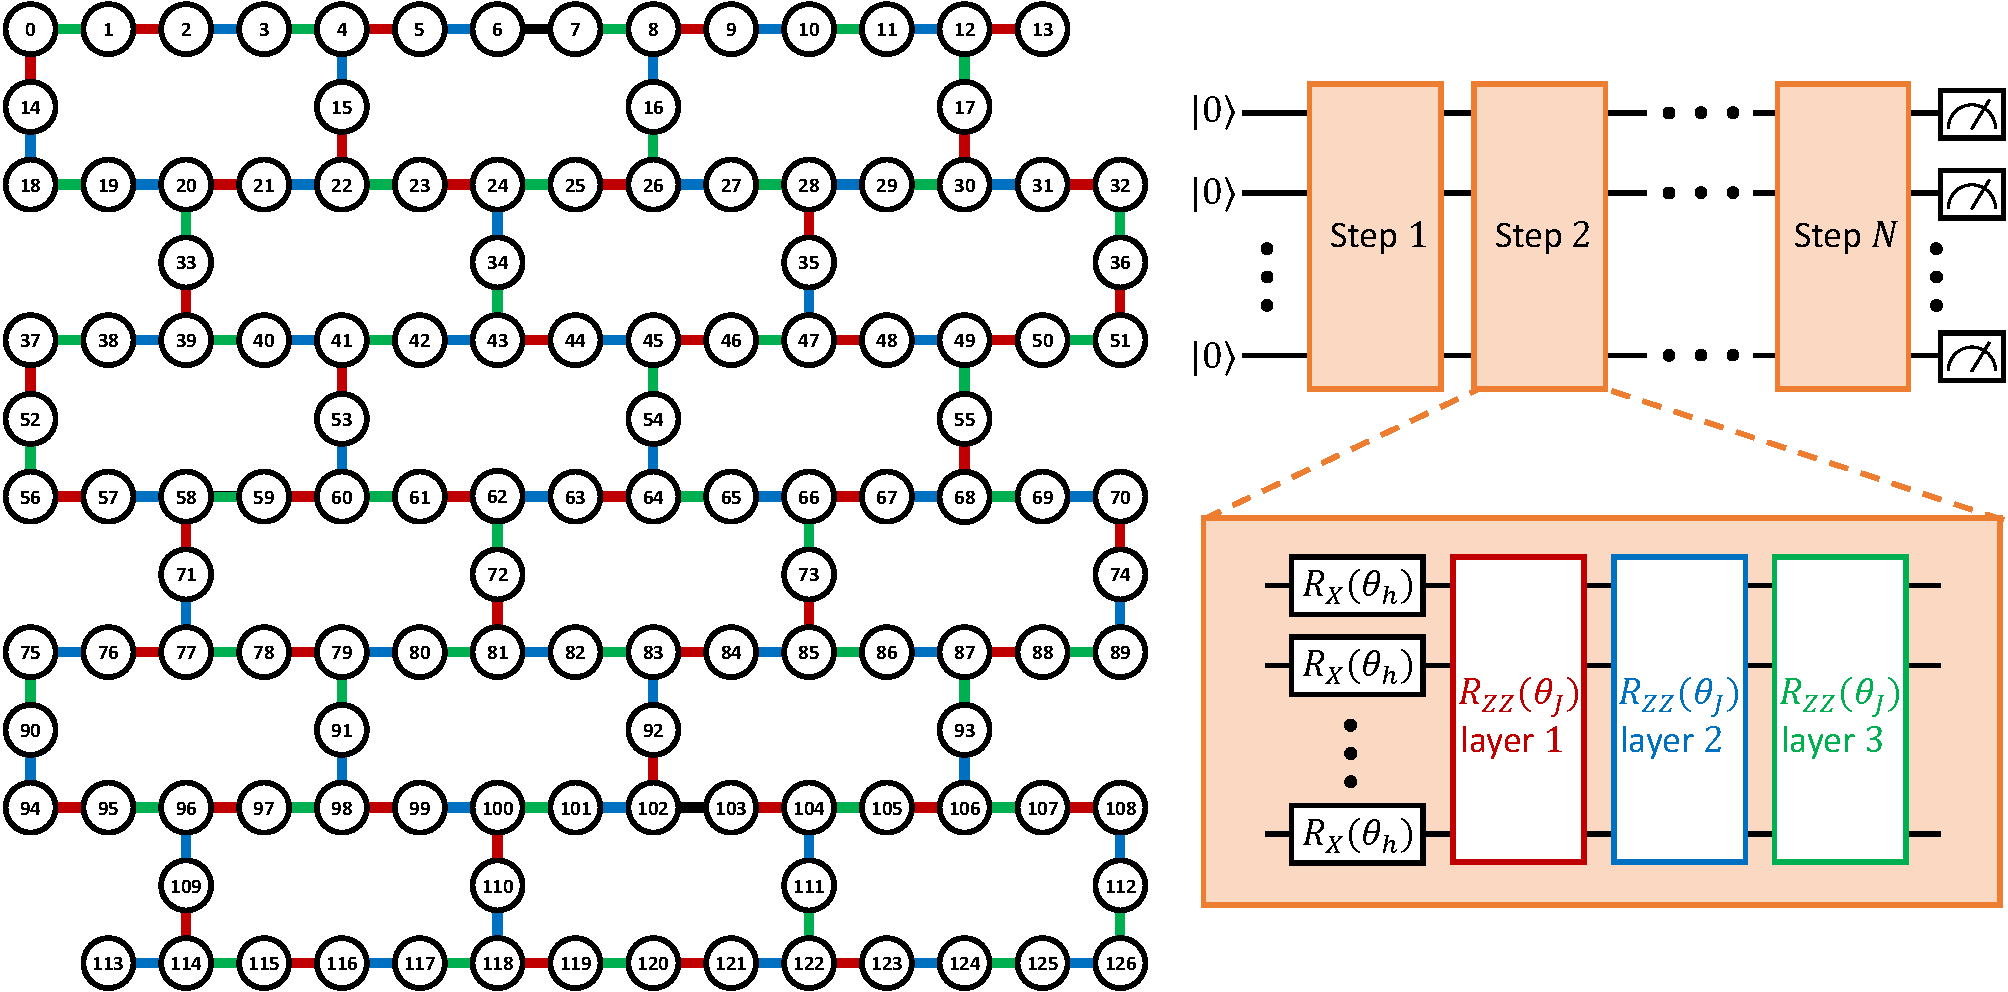
\includegraphics[width=\textwidth]{figures/IBM_Ansatz.pdf}
    \caption{IBM的哈密顿量模拟实验所用的线路}\label{fig:IBM_Ansatz}
\end{figure}

%我们在56核Xeon CPU上使用深度优先搜索策略生成有效路径列表。
在模拟算法的实现中,我们首先使用~\ref{sec:obppp}中描述的反向传播方法找到所有满足条件$\abs{s}\leq M$且具有非零贡献的Pauli路径。随后,我们根据命题~\ref{prop:layer_terms}将这些Pauli路径的贡献函数转换为三角多项式。最后,通过为三角多项式代入不同旋转角度并求和来计算期望值。
值得注意的是,这些Pauli路径贡献实际上表示为$\theta_h$的解析表达式,使我们能够在单次计算中获得整个连续区间内的所有$\theta_h$对应的结果。

使用引理~\ref{lemma:noise},我们可以直接基于贡献的解析表达式计算含噪声量子线路的测量期望值。
这使我们能够直接拟合误差缓解前的原始实验数据。
据我们所知,这是目前唯一能够实现这一目标的经典算法。

%在正文中的图~\ref{fig:IBM}中,我们比较了我们的方法与IBM实验结果在误差缓解(零噪声外推)前后的结果。
为了比较原始实验数据的结果,我们使用经典优化器最小化实验数据集$\{(\theta_h,y_{\theta_h})\}$与我们的近似噪声成本函数$\widehat{\langle O \rangle}$之间的距离,形式化为
\begin{equation}\label{ap:eq:minimal_lambda}
  \lambda=\arg\min_\lambda  \sqrt{\sum_{(\theta_h,y_{\theta_h})\in \mathrm{data set}}\abs{\widehat{\langle O \rangle}(\theta_h)-y_{\theta_h}}^2}.
\end{equation}
在模拟中,我们使用集成在scipy包中的SLSQP优化器来找到$\lambda$~\cite{2020SciPy-NMeth}。


\begin{figure}[htbp]
    \centering
    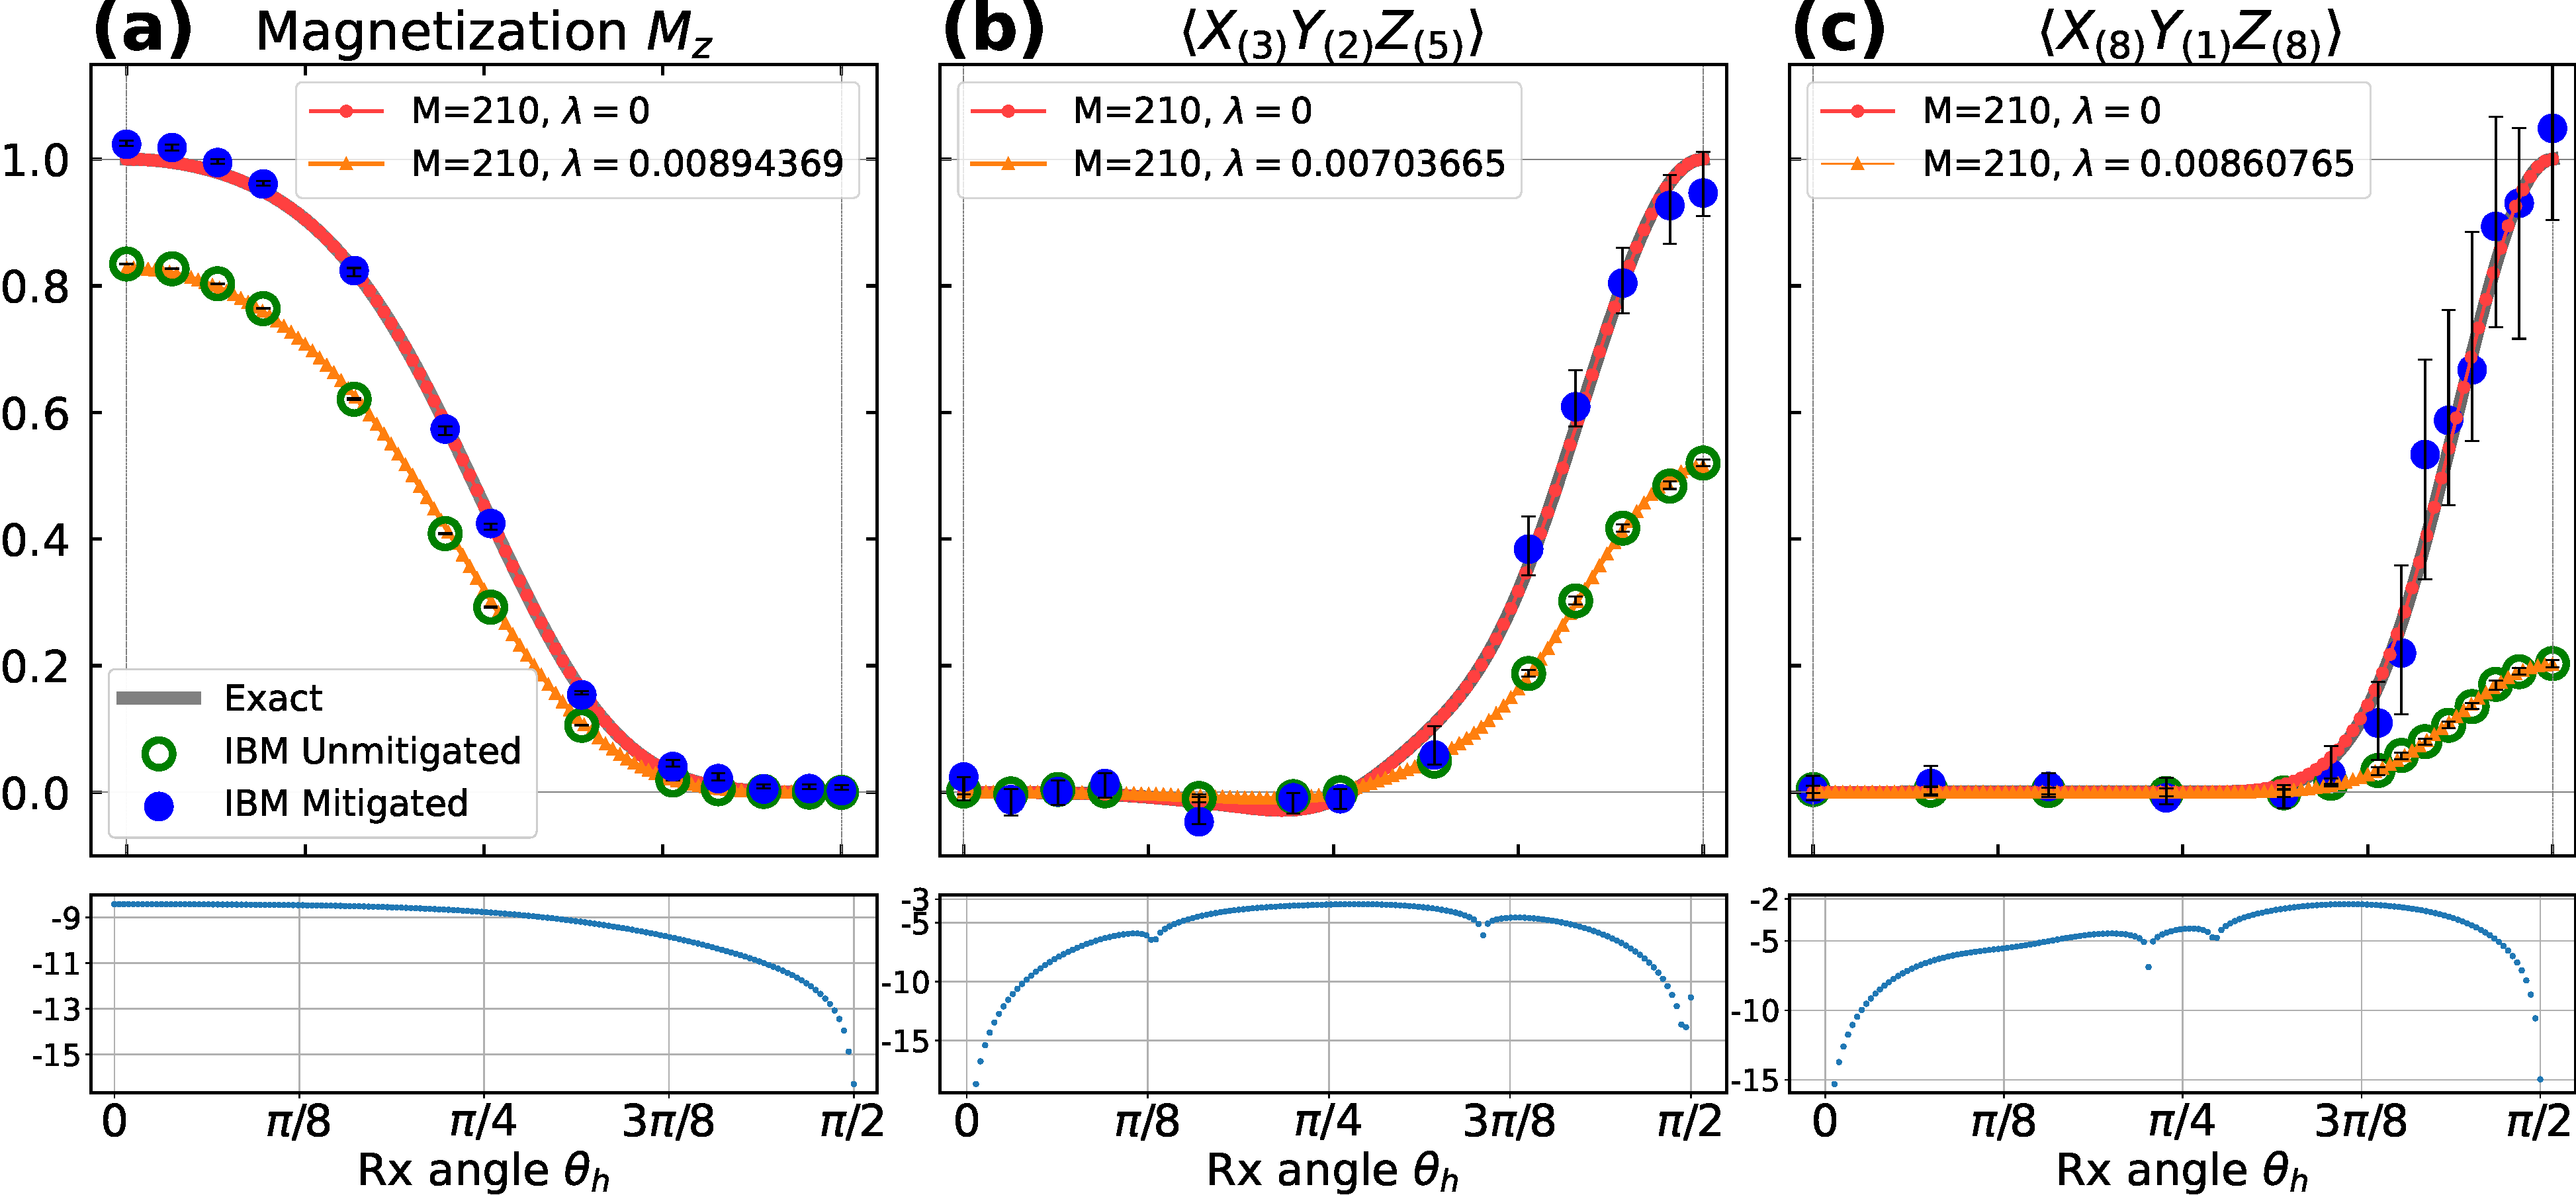
\includegraphics[width=\textwidth]{figures/IBM_F3}
    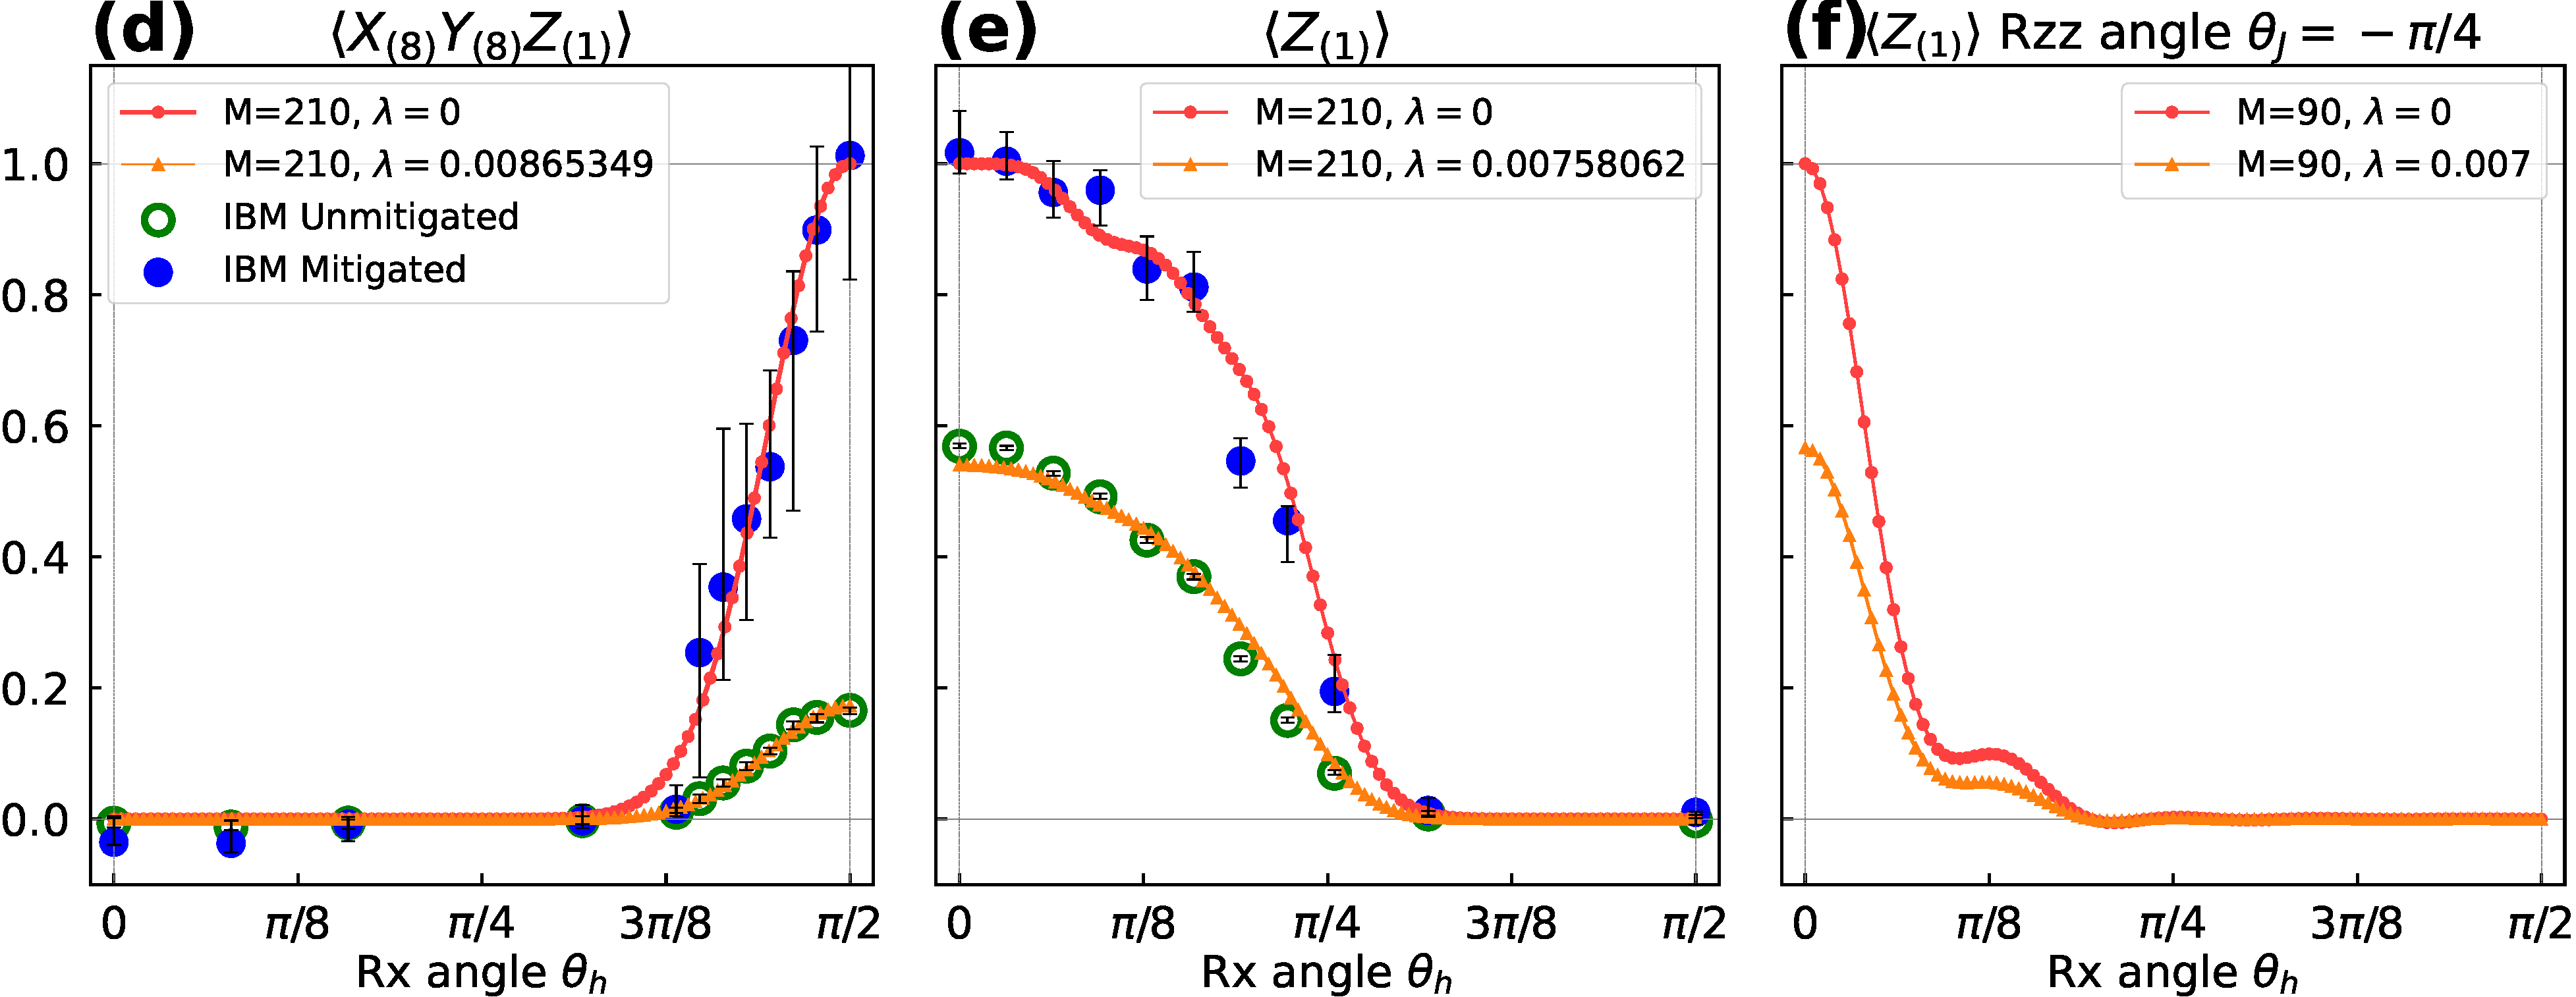
\includegraphics[width=\textwidth]{figures/IBM_F4}
    \caption{IBM的Ising模型演化实验的模拟结果}\label{fig:IBM}
\end{figure}


图~\ref{fig:IBM}展示了IBM在127量子比特Eagle处理器上进行的Ising模型演化实验以及对应的模拟结果。
其中包含了对六种不同实验设定,每种设定的实验量子线路描述如下:
\begin{enumerate}
    \item 在图(a)-(c)中,Trotter步数设为$N=5$,对应于深度为$L=20$的电路。并分别在Hamming Weight 为 $1,10,17$的Pauli算符上进行测量。
    \item 在图(d)中,Trotter步数设为$N=5$,并在电路末尾添加了一层$R_{X}$门,对应于深度为$L=21$的电路。并在Hamming Weight 为 $17$的Pauli算符上进行测量。
    \item 在图(e)中,Trotter步数设为$N=20$,对应于深度为$L=80$的电路。并在Hamming Weight 为 $1$的Pauli算符上进行测量。
    \item 在图(f)中,我们将$R_{ZZ}$门的旋转角设为$\theta_J=-\frac{\pi}{4}$,Trotter步数设为$N=20$,对应于深度为$L=80$的电路。并在Hamming Weight 为 $1$的Pauli算符上进行测量。
\end{enumerate}
图(a)-(e)中的$R_{ZZ}$门的旋转角$\theta_J$设为$\theta_J=-\pi/2$,而(f)中$R_{ZZ}$门的旋转角取自文献~\cite{anand2023classical},设为$\theta_J=-\pi/4$。

图(a)-(e)中的绿色环和蓝色圆分别对应于文献~\cite{kim2023evidence}中报告的不同Pauli算符的直接实验观测结果和经过零噪声推断(Zero-Noise Extrapolation,ZNE)的误差缓解结果。
图(a)-(c)的底部子图显示了OBPPP模拟结果与文献~\cite{kim2023evidence}中呈现的理想精确结果之间的绝对差异。
在每个图中,红点线表示OBPPP模拟的无噪声输出,是关于$\theta_h$三角多项式的解析表达式。
橙色三角线表示在某些噪声抑制下使用截断路径积分近似的含噪声测量期望值。
图(a)-(f)在两颗Xeon 6330 CPU(每颗芯片28核)上的运行时间分别在13秒、146秒、29秒、137秒、262秒和57秒以内。

图(a)-(e)的设定来自文献~\cite{kim2023evidence},(f)的设定来自文献~\cite{anand2023classical}。对于(a)-(c),无噪声理想结果存在精确解,我们发现OBPPP模拟算法(M=210)输出的结果在精度和速度上均优于量子设备~\cite{beguvsic2023fast, kim2023evidence}。
对于(d)-(e),暂时无法获得精确解,所以难以比较无噪声的理想测量期望值,但是可以看到OBPPP的输出结果与IBM的缓解结果非常接近。
在(f)的设定下,暂时缺乏精确结果和实验结果作为比较。
对于(a)-(e),我们使用最小二乘法优化噪声率($p_x=p_y=p_z=\frac{\lambda}{4}$),以拟合噪声电路的期望值。可以看到OBPPP的含噪声期望值模拟结果与IBM未缓解结果之间的强一致性,平均偏差在图(a)-(d)中低于$0.002$,在(e)中均低于$0.008$。优化后的噪声率$\lambda$的范围处于$0.007$到$0.009$,也与IBM报告的误差率一致。



与其他最近的经典模拟算法~\cite{tindall2023efficient,beguvsic2023fast}相比,我们的方法具有两个主要优势:能够获得$\theta_h$的解析表达式,并能够推断含噪声量子线路电路的测量期望值。与张量网络方法~\cite{tindall2023efficient}相比,OBPPP在(b)和(c)中表现出更高的准确性。
在(a)-(e)的所有情况下,OBPPP还表现出更快的执行时间,特别是在更深的电路中~\cite{tindall2023efficient}。
此外,一个显著的区别是,OBPPP在计算(f)时,受到角度变更$\theta_J=\frac{-\pi}{4}$的影响较小。


模拟过程的更多信息和运行时间如表~\ref{tab:IBM}所示:
\begin{table}[h!]
  \centering
  \scalebox{0.6}{
\begin{tabular}{|c|c|c|c|c|c|c|c|c|}
  \hline
    图 & 量子比特数 & 可观测量 & Trotter步数 & 电路深度 & M & 运行时间(56核)&$\min_\lambda  \sqrt{\sum\abs{\widetilde{\langle O \rangle}(\theta_h)-y_{\theta_h}}^2}/\text{\# 数据集}$\\
  \hline
  (a) &127& $M_Z=\sum_q Z_q/n$ &5 & 20 & 210  & 13s&0.0015892257500055675\\
  \hline
  (b) &127& $X_{13,29, 31}Y_{9, 30}Z_{8, 12, 17, 28, 32}$ & 5& 20 & 210  & 146s&0.001395021411390668\\
  \hline
  (c) &127& $X_{37, 41, 52, 56, 57, 58, 62, 79}Y_{75}Z_{38, 40, 42, 63, 72, 80, 90, 91}$ & 5& 20 & 210  & 29s&0.0007674113478406952\\
  \hline
  (d) &127& $X_{37, 41, 52, 56, 57, 58, 62, 79}Y_{38, 40, 42, 63, 72, 80, 90, 91}Z_{75}$ &5& 21 & 210  & 137s&0.0018301118556860437\\
  \hline
  (e) &127& $Z_{63}$ &20& 80 & 210  & 262s&0.007527499236555272\\
  \hline
  (f) &127& $Z_{63}$ &20& 80,$\theta_J=-\pi/4$ & 90  & 57s&\\
  \hline
\end{tabular}}
\caption{IBM的Ising模型演化任务的比较和经典模拟的运行时间}\label{tab:IBM}
\end{table}


\section{QAOA算法实验}


    在上一节中,我们进行了IBM的Ising模型演化实验的模拟,IBM的实验运行一个典型的超导量子比特系统中。
    在本节中,我们将模拟文献~\cite{pagano2020quantum}中报告的离子阱系统的实验结果,并得到高度一致的结果。
    
    在实验中,作者使用了一维排列的$^{171}$Yb$^+$离子,并使用该离子系统实现了低深度长程的量子近似优化算法(QAOA)的演示实验。
    在该QAOA算法中,优化问题被编码在具有长程相互作用的横场反铁磁Ising模型哈密顿量中:
    \begin{equation}\label{eq:qaoa:hamiltonian}
        H=\underbrace{\sum_{i<j}J_{ij}X_iX_j}_{H_A}+\underbrace{B\sum_iY_i}_{H_B}.
    \end{equation}
    其中,$J_{i,j}>0$表示自旋$i$和$j$之间的Ising耦合强度,随自旋间距离按幂律衰减;$B$表示横向磁场强度。为了方便我们将$\sum_{i<j}J_{ij}X_iX_j$记为$H_A$,$B\sum_iY_i$记为$H_B$。
    
    系统的初态度经过$p$层QAOA线路块演化后的状态为:
    \begin{equation}
      \ket{\vec{\beta},\vec{\gamma}}=\prod_{k=1}^p e^{-i\beta_k (H_B/J_0)} e^{-i\gamma_k (H_A/J_0)}\ket{\psi_0},
    \end{equation}
    其中$J_0$是最近邻耦合的平均值,角度向量$\vec{\beta}$和$\vec{\gamma}$是用于最小化最终能量的变分参数:
    \begin{equation}
      E(\vec{\beta},\vec{\gamma})=\bra{\vec{\beta},\vec{\gamma}}H\ket{\vec{\beta},\vec{\gamma}}。
    \end{equation}
    初始状态设为$\ket{\psi_0}=\ket{\uparrow\uparrow\dots\uparrow}_Y$,其中$\ket{\uparrow}_Y=(\ket{\uparrow}_Z+i\ket{\downarrow}_Z)/\sqrt{2}$。
    
    在原实验设定中,作者使用无量纲相对量:
    \begin{equation}\label{ap:eq:qaoa:eta}
      \eta=\frac{E(\vec{\beta},\vec{\gamma})-E_{\max}}{E_{gs}-E_{\max}}
    \end{equation}
    来衡量QAOA算法输出结果的表现,其中$E_{gs}$是哈密顿量~\eqref{eq:qaoa:hamiltonian}的基态能量,$E_{\max}$表示最高激发态的能量。
    
    在本节中,我们将使用OBPPP算法模拟文献~\cite{pagano2020quantum}中图2C的实验结果。
    在该实验中,量子比特数为$n=12$,QAOA线路块的层数为$p=1$。
    在我们的模拟过程中,Ising模型的耦合强度$J_{ij}$设为文献~\cite{pagano2020quantum}补充信息中给出的解析拟合形式:
    \begin{equation}
      J_{ij}\approx\frac{J_0}{r^{\alpha^\prime}}e^{-\beta^\prime(r-1)},
    \end{equation}
    其中$J_0$是最近邻耦合的平均值,$r=\abs{i-j}$是离子间距,$\alpha^\prime,\beta^\prime$是指数衰减变量。
    根据参考文献中的设定,$J_0=0.580$,$\alpha^\prime=0.322$,$\beta^\prime=0.229$,横向磁场满足$B/J_0=-0.25$。
    
    \begin{figure}[hbp]	
        \centering
        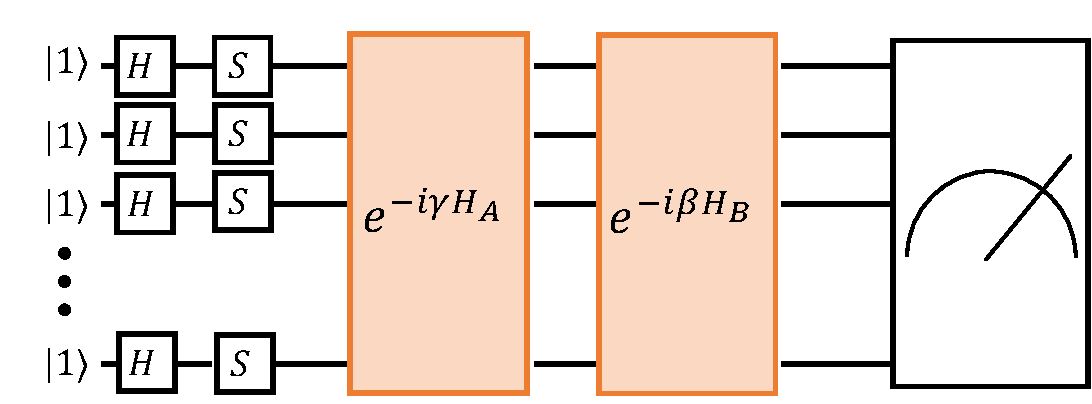
\includegraphics[width=0.75\textwidth]{figures/Ion_ansatz.pdf}
        \caption{QAOA实验模拟中使用的12量子比特电路}\label{fig:Ion_Ansatz}
    \end{figure}
    
    模拟中使用的电路如图~\ref{fig:Ion_Ansatz}所示。通过以下公式:
    \begin{equation}
        SH\ket{1}=S(\ket{0}-\ket{1})/\sqrt{2}=(\ket{0}-i\ket{1})/\sqrt{2}=-i\ket{\uparrow}_Y,
    \end{equation}
    我们使用初始状态$\ket{1}$并通过一层$H$门和一层$S$门,等效生成实验中的初始状态$\ket{\psi_0}$。
    电路中对应于$H_A$部分的演化:
    \begin{equation}
        e^{-i\gamma (H_A/J_0)}=e^{-i\gamma \sum (J_{ij}/J_0)X_iX_j},
    \end{equation}
    可以通过一系列$R_{XX}$门,利用$\Pi e^{-i\gamma(J_{ij}/J_0)X_iX_j}$来实现。
    因为在实验中总共有$(^{12}_2)=66$对相互作用(或$R_{XX}$门),这些$R_{XX}$门可以按最紧凑的排列方式在电路中使用$66/6=11$层线路实现。
    而演化对应于$H_B$的部分$e^{-i\beta (H_B/J_0)}=e^{-i\beta \sum(B/J_0)Y_i}$,可以由一层作用于每个量子比特的$R_Y$门实现。
    %初始状态$\ket{1}$首先通过一层$H$门和一层$S$门,等效生成实验中的初始状态$\ket{\psi_0}$。
    电路中对应于$H_A$的演化由11层不重叠的$R_{XX}$门实现,对应于$H_B$的演化由一层作用于每个量子比特的$R_Y$门实现,而生成初始态制备需要额外的两层线路,于是电路的总层数为14层。
    
    \begin{figure}[htbp]
        \centering
        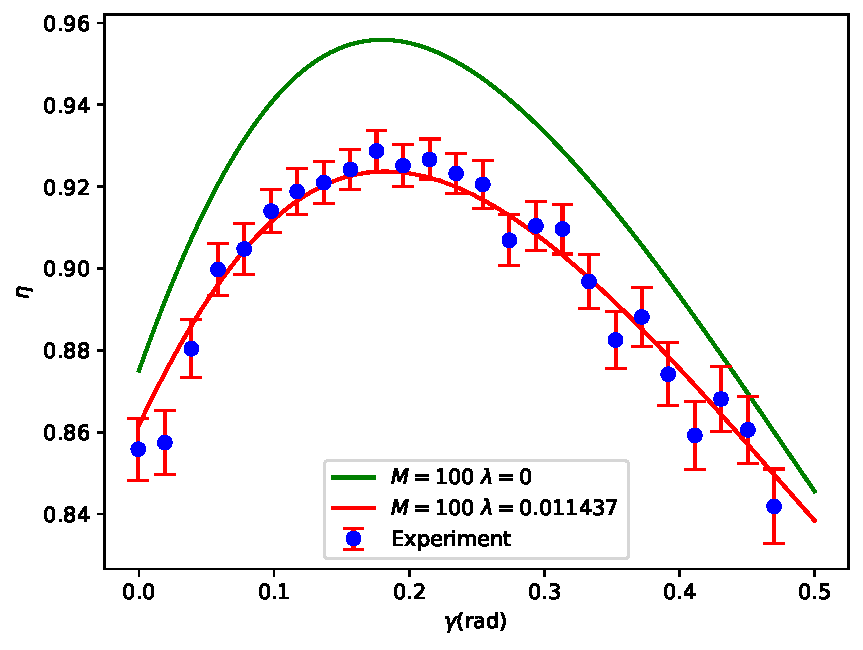
\includegraphics[width=0.95\textwidth]{figures/QAOA.pdf}
        \caption{QAOA实验结果与模拟结果的比较}\label{fig:QAOA_result}
    \end{figure}
    
    在文献~\cite{pagano2020quantum}的图2C中,作者报告了设定角度$\beta^\star=1.12$时,测量期望值视角度$\eta$为变分参数$\gamma$的函数的实验结果。
    模拟结果如图~\ref{fig:QAOA_result}所示,y轴$\eta$定义在式~\ref{ap:eq:qaoa:eta}中。
    为了模拟退极化噪声$p_x = p_y = p_z = \frac{\lambda}{4}$存在时的含噪声测量期望值结果,类似于前一节,我们使用SLSQP优化器优化式~\ref{ap:eq:minimal_lambda}以获得合适的噪声率$\lambda$来拟合实验结果。
    优化后所得的最佳噪声率为$\lambda=0.011437$。
    从图中可以看出,噪声的出现影响了QAOA的性能,实验结果相比于无噪声推测结果略低。
    与实验结果相比较,在这个离子阱系统实验中,我们的方法很好地拟合了含噪声的实验结果,表明OBPPP方法在实际应用中具有很好的适用性。



\section{本章小结}

在本章中,我们通过数值模拟验证了基于Pauli路径积分的量子线路模拟算法在多种实际场景中的有效性和效率。主要研究成果总结如下:
\begin{enumerate}
    \item 含噪变分线路的复杂度验证:通过系统性的数值实验,我们发现具有非零贡献的Pauli路径数量随线路深度$L$呈现先增后减的趋势,与理论预测一致。实际路径数量显著低于理论上限$\mathrm{Poly}(n)2^M$,表明算法具有更高的实用效率。对于实际常用的量子线路,当噪声率$\lambda<0.05$时,实现$99.9\%$精度仅需截断数$M\approx34$,远低于理论估计的$M\sim5000$。因此对于实际应用中的含噪声量子线路模拟,OBPPP的实际运行效率远高于理论分析的多项式界限。
    \item Clifford扰动线路的误差特性:在硬件高效线路上的基准测试表明,SPD模拟器在$\theta_*=\pi/20$的小角度空间内可将误差控制在$10^{-2}$以内。对于$n=15$量子比特系统,$M=11$时截断误差在$\theta_*=\pi/8$范围内仍保持$<0.01$,展现了算法的鲁棒性。
    \item 大规模量子系统的模拟能力:在IBM 127量子比特Ising模型演化实验中,OBPPP算法成功复现了原始实验数据,与未缓解结果的平均偏差低于$0.008$。y与IBM的量子计算机相比,OBPPP算法单次计算即可获得关于$\theta_h$的解析表达式,在计算精度和速度上均具有显著优势。
    \item 离子阱量子系统的实验验证:在12量子比特QAOA实验中,通过优化得到噪声率$\lambda=0.0114$,模拟结果与离子阱实验数据高度吻合。验证了算法对长程相互作用和非均匀耦合强度的适应性。
\end{enumerate}


这些数值实验结果表明,基于Pauli路径积分的模拟算法不仅具有严格的理论保证,在实际应用中更能突破理论分析的保守估计,为含噪声量子线路的经典模拟提供了高效可行的解决方案。特别是对超大规模($n>100$)量子系统的模拟能力,为量子-经典混合计算范式的验证和量子优越性实验的基准测试提供了重要工具,具有广泛的应用前景和实用性。


% 其他部分
\backmatter

% 参考文献
\bibliography{ref/refs}  % 参考文献使用 BibTeX 编译
% \printbibliography       % 参考文献使用 BibLaTeX 编译

% 附录
% 本科生需要将附录放到声明之后,个人简历之前
\appendix
% \input{data/appendix-survey}       % 本科生:外文资料的调研阅读报告
% \input{data/appendix-translation}  % 本科生:外文资料的书面翻译
% !TeX root = ../thuthesis-example.tex

\chapter{补充内容}

附录是与论文内容密切相关、但编入正文又影响整篇论文编排的条理和逻辑性的资料,例如某些重要的数据表格、计算程序、统计表等,是论文主体的补充内容,可根据需要设置。

附录中的图、表、数学表达式、参考文献等另行编序号,与正文分开,一律用阿拉伯数字编码,
但在数码前冠以附录的序号,例如“图~\ref{fig:appendix-figure}”,
“表~\ref{tab:appendix-table}”,“式\eqref{eq:appendix-equation}”等。


\section{插图}

% 附录中的插图示例(图~\ref{fig:appendix-figure})。

\begin{figure}
  \centering
  \includegraphics[width=0.6\linewidth]{example-image-a.pdf}
  \caption{附录中的图片示例}
  \label{fig:appendix-figure}
\end{figure}


\section{表格}

% 附录中的表格示例(表~\ref{tab:appendix-table})。

\begin{table}
  \centering
  \caption{附录中的表格示例}
  \begin{tabular}{ll}
    \toprule
    文件名          & 描述                         \\
    \midrule
    thuthesis.dtx   & 模板的源文件,包括文档和注释 \\
    thuthesis.cls   & 模板文件                     \\
    thuthesis-*.bst & BibTeX 参考文献表样式文件    \\
    thuthesis-*.bbx & BibLaTeX 参考文献表样式文件  \\
    thuthesis-*.cbx & BibLaTeX 引用样式文件        \\
    \bottomrule
  \end{tabular}
  \label{tab:appendix-table}
\end{table}


\section{数学表达式}

% 附录中的数学表达式示例(式\eqref{eq:appendix-equation})。
\begin{equation}
  \frac{1}{2 \uppi \symup{i}} \int_\gamma f = \sum_{k=1}^m n(\gamma; a_k) \mathscr{R}(f; a_k)
  \label{eq:appendix-equation}
\end{equation}


\section{文献引用}

附录中的参考文献引用

\printbibliography


% 致谢
% !TeX root = ../thuthesis-example.tex

\begin{acknowledgements}
  我谨向我的导师刘正伟表示衷心的感谢,他引领我进入了一个全新的数学研究世界。没有他持续的支持、鼓励、耐心和专业建议,这项工作无法完成。

  我还要要感谢数学中心的魏朝晖、刘子文、刘锦鹏、丁大威老师他们在同我的讨论中给予了我很多帮助。
  以及雁栖湖应用中心的程嵩老师,这项工作的一部分是在他的指导下完成的。


  最后,我要感谢我的伙伴们——陆凡、魏付川、张浩、赵子硕、李俊峰、阮钰泽、王宁烽、卢润迪、何会萱、张睿齐,以及清华的朋友们,感谢他们与我一起讨论了许多精彩的数学问题。
\end{acknowledgements}


% 声明
% 本科生开题报告不需要
\statement
% 将签字扫描后的声明文件 scan-statement.pdf 替换原始页面
% \statement[file=scan-statement.pdf]
% 本科生编译生成的声明页默认不加页脚,插入扫描版时再补上;
% 研究生编译生成时有页眉页脚,插入扫描版时不再重复。
% 也可以手动控制是否加页眉页脚
% \statement[page-style=empty]
% \statement[file=scan-statement.pdf, page-style=plain]

% 个人简历、在学期间完成的相关学术成果
% 本科生可以附个人简历,也可以不附个人简历
% !TeX root = ../thuthesis-example.tex

\begin{resume}

  \section*{个人简历}

  1997 年 11 月 11 日出生于四川省自贡市。

  2016 年 9 月考入华中科技大学数学与统计学院数学与应用数学专业,2020 年 6 月本科毕业并获得理学学士学位。

  2020 年 9 月免试进入清华大学数学科学系攻读数学博士至今。


  \section*{在学期间完成的相关学术成果}

  \subsection*{学术论文}

  \begin{achievements}
    \item Shao, Y., Wei, F., Cheng, S., \& Liu, Z. (2024). Simulating noisy variational quantum algorithms: A polynomial approach. Physical Review Letters, 133(12), 120603.
    \item Sun, W., Wei, F., Shao, Y., \& Wei, Z. (2024). Sudden death of quantum advantage in correlation generations. Science Advances, 10(47), eadr5002.
    \item Huang, Y., Shao, Y., Ren, W., Sun, J., \& Lv, D. (2023). Efficient quantum imaginary time evolution by drifting real-time evolution: An approach with low gate and measurement complexity. Journal of Chemical Theory and Computation, 19(13), 3868-3876.
    \item Shao, Y., Li, Y., Wei, F., Zhan, H., Wang, B., Wei, Z., Zhang, L., \& Liu, Z. (2024). Variational Graphical Quantum Error Correction Codes: adjustable codes from topological insights. arXiv preprint arXiv:2410.02608.
    \item Zhang, R., Shao, Y., Wei, F., Cheng, S., Wei, Z., \& Liu, Z. (2024). Clifford Perturbation Approximation for Quantum Error Mitigation. arXiv preprint arXiv:2412.09518.
  \end{achievements}

  %\subsection*{专利}

  %\begin{achievements}
    %\item 任天令, 杨轶, 朱一平, 等. 硅基铁电微声学传感器畴极化区域控制和电极连接的方法: 中国, CN1602118A[P]. 2005-03-30.
    %\item Ren T L, Yang Y, Zhu Y P, et al. Piezoelectric micro acoustic sensor based on ferroelectric materials: USA, No.11/215, 102[P]. (美国发明专利申请号.)
  %\end{achievements}

\end{resume}


% 指导教师/指导小组评语
% 本科生不需要
% !TeX root = ../thuthesis-example.tex

\begin{comments}
% \begin{comments}[name = {指导小组评语}]
% \begin{comments}[name = {Comments from Thesis Supervisor}]
% \begin{comments}[name = {Comments from Thesis Supervision Committee}]

  %论文提出了……
  暂无

\end{comments}


% 答辩委员会决议书
% 本科生不需要
% !TeX root = ../thuthesis-example.tex

\begin{resolution}
  经典模拟是研究量子算法、量子纠错、校准量子计算机的重要工具。现如今随着量子硬件的发展,传统的经典模拟方法已经逐渐逼近性能极限。在当前的时代背景下,变分量子算法因为不需要昂贵的纠错协议受到了广泛关注,但变分量子算法能否在线路噪声等实际环境下实现量子优势仍然是个困难的、被反复讨论的开放问题。

邵钰菓的博士学位论文《基于Pauli路径积分模拟量子线路》聚焦NISQ时代量子线路的经典模拟难题,提出了基于Pauli路径积分的泡利基下反向路径积分(OBPPP)算法并拓展了稀疏泡利动力学(SPD)算法,系统分析了算法的计算复杂度与误差特性,揭示了噪声对量子优势边界的临界影响。论文的主要成果如下:


1. 证明了绝大多数含噪声变分量子线路观测期望值在一定条件下的经典可模拟性。

2. 证明了在Pauli噪声率恒定或高于1/logL时,观测期望值可被多项式复杂度经典模拟;而当噪声率低于1/L时,模拟复杂度可能指数增长。

3. 通过复现IBM 127量子比特Eagle处理器的Ising模型实验,验证了该模拟算法在精度与效率上显著优于实际量子设备,并实现了噪声强度的量化评估。

研究兼具理论深度与实践价值,为量子硬件验证及噪声抑制提供了重要工具。


论文选题前沿,逻辑严谨,成果发表于《Physical Review Letters》等高水平期刊,创新性突出,理论意义与应用价值显著。答辩过程中,邵钰菓陈述清晰,表达严谨,准确回答了委员会提出的问题,展现了扎实的专业功底与独立科研能力。


经答辩委员会讨论与无记名投票,一致通过邵钰菓的博士学位论文答辩,认为这是一篇优秀的博士学位论文,建议授予邵钰菓理学博士学位。


\end{resolution}


% 本科生的综合论文训练记录表(扫描版)
% \record{file=scan-record.pdf}

\end{document}
